\documentclass[Total.tex]{subfiles}
\usepackage{stmaryrd}
\begin{document}
	\chapter{Fundamental Groups}
		\section{Definitions}
			\begin{Def}
				Let $X$ be a topological space:
				\begin{itemize}
					\item We define a \textbf{path} in $X$ as a continuous map
					\begin{gather*}
						\gamma:[a,b]\rightarrow X
					\end{gather*}
					often we say: $\gamma(a)$ is the \textbf{starting point} and $\gamma(b)$ si the \textbf{end point}.
					\item A \textbf{loop} is a path with $\gamma(a)=\gamma(b)$;
					\item Given a path $\gamma:[a,b]\rightarrow X$, define its inverse 
					\begin{gather*}
						\bar{\gamma}:[a,b]\rightarrow X\qquad t\mapsto \gamma(b+a-t)
					\end{gather*}
				\end{itemize}
			\end{Def}
			
			\subsection{Path-Homotopy}
				\begin{Def}
					Let $X$ be a topological space:
					\begin{itemize}
						\item Let $\gamma_0,\gamma_1:[a,b]\rightarrow X$ be two paths with the same starting point $P$, and the same end point $Q$.
						
						A \textbf{path homotopy} between the paths $\gamma_0,\gamma_1$ is a homotopy rel $\{a,b\}$ between $\gamma_0$ and $\gamma_1$.
						
						In other words, a path-homotopy is a continuous map
						\begin{gather*}
							\Gamma:[a,b]\times [0,1]\rightarrow X
						\end{gather*}
						Such that
						\begin{gather*}
							\Gamma(t,0)=\gamma_0(t)\qquad \Gamma(t,1)=\gamma_1(t)\\
							\Gamma(a,s)=P\qquad \Gamma(b,s)=Q
						\end{gather*}
						\item If $\gamma_0$ and $\gamma_1$ are path-homotopic, then written as $\gamma_0\simeq_p \gamma_1$;
						\item Especially, a loop $\gamma$ is \textbf{null-homotopic}, if it is path-homotopic to the constant path $\delta$ given by
						\begin{gather*}
							\delta(t):=\gamma(a)
						\end{gather*}
					\end{itemize}
				\end{Def}
				\subsubsection{Reparametrization}
				\begin{Def}
					Let $\gamma:[a,b]\rightarrow X$ be a path in topological space $X$, and let
					\begin{gather*}
						\varphi:[a,b]\rightarrow [a,b]
					\end{gather*}
					which satisfies:
					\begin{itemize}
						\item Continuous;
						\item $\gamma(a)=a;\gamma(b)=b$;
						\item Monotone;
					\end{itemize}
				\end{Def}
					\begin{lemma}
						(Reparametrization-Homotopy Lemma) Let $\gamma:[a,b]\rightarrow X$ be a path in a topological space $X$.
						
						If: a path $\delta:[a,b]\rightarrow X$ is obtained from $\gamma$ by a reparametrization, then
						\begin{gather*}
							\gamma\simeq_p \delta
						\end{gather*}
					\end{lemma}
					\begin{proof}
						Firstly,consider the reprametrization $\gamma:[a,b]\rightarrow [a,b]$. Then
						\begin{gather*}
							F:[a,b]\times [0,1]\rightarrow X\\
							(t,s)\mapsto \gamma(t+(1-s)\varphi(t))
						\end{gather*}
						is a path homotopy.
					\end{proof}
					\begin{lemma}
						(Path-Homotopy Equivalence Lemma) Let $X$ be topological space and $x,y\in X$. Then,path-homotopy is an equivalence relation on the set of paths $[a,b]\rightarrow X$.
					\end{lemma}
					\begin{proof}
						内容...
					\end{proof}
				\subsubsection{Homotopy Class}
					
					\begin{lemma}
						内容...
					\end{lemma}
					\begin{proof}
						内容...
					\end{proof}
					\begin{Def}
						\begin{itemize}
							\item (Homotopy Class)
							\item (Product)
						\end{itemize}
					\end{Def}
					\begin{proposition}
						(Path-Homotopy Product Proposition)
					\end{proposition}
				\subsubsection{The Fundamental Group of Pointed Topological Space}
					\begin{Def}
						内容...
					\end{Def}
					\begin{proposition}
						($\pi_1$-Group Proposition) Let $X$ be a topological space and $x_0\in X$, the set
						\begin{gather*}
							\pi_1(X,x_0):=\{\mbox{path-homotopy classes of loops in }(X,x_0)\}
						\end{gather*}
						together with
					\end{proposition}
					\begin{proof}
						内容...
					\end{proof}
					
					\begin{Def}
						内容...
					\end{Def}
				\subsubsection{Change of Base Points}	
					\begin{proposition}
						(Change of Base Point Propsition)
					\end{proposition}
					\begin{proof}
						内容...
					\end{proof}
					
					\begin{corollary}
						内容...
					\end{corollary}
					\begin{proof}
						内容...
					\end{proof}
				\subsubsection{Examples}
				\begin{itemize}
					\item Fundamental Group of the circle:
					\begin{lemma}
						(Lesbegue's Lemma) Let
						\begin{gather*}
							f:[0,1]^m\rightarrow X
						\end{gather*}
						
						be a continuous map. Let $\{V_i\}$ be an open cover of $X$. 
						
						Then, for every $a_1,\dots,a_m\in \{0,1,\dots,N-1\}$there exists an $N\in \NN$ such that
						\begin{gather*}
							f([\frac{a_1}{N},\frac{a_1+1}{N}]\times\dots\times [\frac{a_m}{N},\frac{a_m+1}{N}])\subseteq V_i
						\end{gather*}
					\end{lemma}
					\begin{proof}
						Here: 
					\end{proof}
					\begin{Def}
						\begin{itemize}
							\item Consider map $\Xi:\RR\rightarrow S^1$;
							\item Let $X$ be a topological space with $f:X\rightarrow S^1$ continuous.
							
							A \textbf{lift} of $f$ is a continuous map
							\begin{gather*}
								\tilde{f}:W\rightarrow \RR
							\end{gather*}
							such that $\Xi\circ \tilde{f}=f$. In other words, such that for all $w\in W$ we have
							\begin{gather*}
								f(w)=exp(i\cdot \tilde{f}(w))
							\end{gather*}
							\begin{center}
								\begin{tikzcd}
									&\RR\arrow[d,"p"]\\
									W\arrow[ru,"\tilde{f}"]\arrow[r,"f"]&S^1
								\end{tikzcd}
							\end{center}
						\end{itemize}
					\end{Def}
					
					\begin{example}
						(Lift) Consider the map $f:[0,1]\rightarrow S^1,t\mapsto exp(2\pi int)$. Then, consider the lift given by
						\begin{gather*}
							\tilde{f}:t\mapsto 2\pi in\cdot t
						\end{gather*}
						The lift is not unique, take $k=2\pi\cdot n$.
					\end{example}
					
					\begin{lemma}
						(Lift Uniqueness Lemma) Let $W$ be a connected topological space. Let $f:W\rightarrow S^1$ be a continuous map and $\tilde{\varphi},\tilde{\psi}:W\rightarrow \RR$ be two lifts of $f$.
						
						If $\tilde{\varphi},\tilde{\psi}$ agrees on some point $w_0\in W$, then they agree everywhere. 
					\end{lemma}
					\begin{proof}
						Consider the following map
						\begin{gather*}
							\theta:W\rightarrow \RR\qquad w\mapsto \theta(w):=\tilde{\varphi}(w)-\tilde{\psi}(w)
						\end{gather*}
						Then, by hypothesis, we have
						\begin{gather*}
							\theta(w_0)=0\qquad exp(i\theta(w))=f(w)\cdot f(w)^{-1}=1
						\end{gather*}
						
						This implies, that $s\mapsto \theta(w)$ maps $W$ into $2\pi\cdot \ZZ=\Xi^{-1}(1)$. $W$ is connected, so they agrees everywhere.
					\end{proof}
					\begin{lemma}
						(Lift-Extension Lemma) Let $X$ be a topological space, we suppose that we have a decomposition that
						\begin{gather*}
							X=A\cup B\qquad A,B\mbox{ are closed}
						\end{gather*}
						Now, let $f:X\rightarrow S^1$ be continuous, $\tilde{f}:A\rightarrow \RR$ be a lift of $f|A$. We suppose that the following statements hold:
						\begin{itemize}
							\item There exists a $P\in S^1$ with
							\begin{gather*}
								f(B)\subseteq S^1-\{P\}
							\end{gather*}
							\item The intersection $A\cap B$ is \textbf{connected} and \textbf{nonempty}.
						\end{itemize}
						Then, there exists a lift $\tilde{f}:X\rightarrow \RR$ of $f$ agrees with the given lift on $A$.
					\end{lemma}
					\begin{figure}[H]
						\centering
						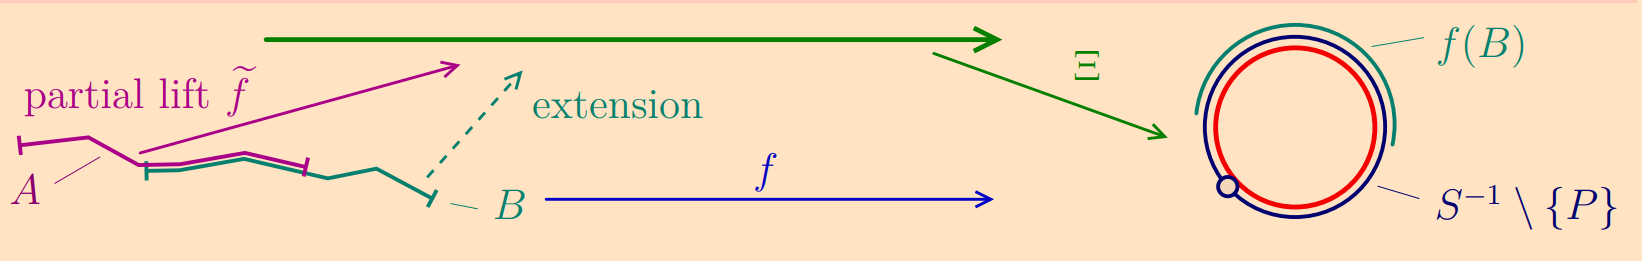
\includegraphics[width=0.8\textwidth]{AT1.png}
					\end{figure}
					\begin{proof}
						Firstly, pick some $x_0\in A\cap B$, and $s\in \RR$ such that $\Xi(s)=P$. Then,
						\begin{gather*}
							f(x_0)\in f(A\cap B)\subseteq f(B)\subseteq S^1-\{P\}\Rightarrow \tilde{f}(x_0)\notin\Xi^{-1}(P) 
							\end{gather*}
							So, there exists some $m\in \ZZ$ such that
							\begin{gather*}
								\tilde{f}(x_0)\in (s+2\pi m,s+2\pi (m+1))
							\end{gather*}
							Then, restriction of $\Xi$ to $(s+2\pi m,s+2\pi(m+1))\rightarrow S^1-\{P\}$ is a homeomorphism. Denote $\Psi:=[\Xi|(s+2\pi m,2+2\pi(m+1))]^{-1}$. 
							
							Now, define
							\begin{gather*}
								\tilde{f}(x):=\begin{cases}
									\tilde{f}(x)&x\in A\\
									\Psi(f(x))&x\in B\Rightarrow f(x)\in S^1-\{P\}
								\end{cases}
							\end{gather*}
							The definition agrees on $A\cap B$: For $x\in A\cap B$,
							\begin{gather*}
								\Psi(f(x))=\tilde{f}(x),x\in A
							\end{gather*}
							
							Thus, the definition of $\tilde{f}$ can be extended to $A\cup B$. 
					\end{proof}
					
					\begin{lemma}
						(Lift from $S^1$ to $\RR$) Given any continuous map 
						\begin{gather*}
							f:[0,1]\rightarrow S^1
						\end{gather*}
						and any $\tilde{y}_0\in \RR$ with
						\begin{gather*}
							f(0)=exp(i\cdot \tilde{y}_0)=\Xi(\tilde{y}_0)
						\end{gather*}
						There exists a \textbf{unique lift} $\tilde{f}:[0,1]\rightarrow \RR$ of $f$ with
						\begin{gather*}
							\tilde{f}(0)=\tilde{y}_0
						\end{gather*} 
					\end{lemma}
					\begin{proof}
						\begin{itemize}
							\item Uniqueness: By Lift Uniqueness lemma.
							\item Existence: Apply Lift-Extension lemma. Decompose the interval $[0,1]$ into smaller intervals, such that: on each subinterval, the image of $f$misses at least one point in $S^1$.
						\end{itemize}
					\end{proof}
					\begin{theorem}
						The map
						\begin{gather*}
							\Psi:\ZZ\rightarrow \pi_1(S^1,1)\qquad \\
							\Theta:\pi_1(S^1,z_0)\rightarrow \ZZ\qquad 
						\end{gather*}
						are well defined, and are isomorphisms of group.
					\end{theorem}
					\begin{proof}
						
					\end{proof}
					\item Lifting of Square:
					\begin{lemma}
						内容...
					\end{lemma}
					\begin{proof}
						内容...
					\end{proof}
					\item Fundamental Group of spheres:
					\begin{lemma}
						(Sphere Minus Point Lemma)For every $P\in S^n$, $S^n-\{P\}$ is simply connected.
					\end{lemma}
					\begin{proof}
						We have $S^n-\{P\}\cong \RR^n$. 
					\end{proof}
					\begin{proposition}
						For $n\geq 2$ we have
						\begin{gather*}
							\pi_1(S^n)=0
						\end{gather*}
						i.e. it is simly connected.
					\end{proposition}
					\begin{proof}
						内容...
					\end{proof}
					
				\end{itemize}
				
				\begin{proposition}
					($\pi_1$-Group Proposition) Let $X$ be a topological space and $x_0\in X$, the set
					\begin{gather*}
						\pi_1(X,x_0):=
					\end{gather*}
					together with product
				\end{proposition}
				\begin{proof}
					内容...
				\end{proof}
				
				\begin{Def}
					内容...
				\end{Def}
			\subsubsection{Alternative Descriptions}
				
			\subsubsection{Change of Base Points}
			\subsection{Applications}
			\subsubsection{The Fundalmental Theorem of Algebra}
			\begin{theorem}
				(TFTA) Every nonconstant polynomial in $\CC[z]$ has a zero in $\CC$.
			\end{theorem}
			\begin{proof}
				内容...
			\end{proof}
			\subsubsection{2D-BOrsuk-Ulam Theorem}
			\subsubsection{Path Integrals, Fundamental Groups}
			\subsection{Functoriality}
			\subsubsection{Group Homomorphisms induced by Continuous Map}
			\begin{Def}
				内容...
			\end{Def}
		\section{Coverings and Fundamental Groups}
			\subsection{Group Action}
			\subsubsection{Klein Bottle as Quotient}
			\begin{lemma}
				内容...
			\end{lemma}
			\begin{proof}
				内容...
			\end{proof}
			\subsection{Covering of Topological Spaces}
			\begin{Def}
				Let $p:X\rightarrow B$ be a continuous map between topological spaces:
				\begin{itemize}
					\item An open subset $U\subseteq B$ is called \textbf{uniformly covered} if 
					\item We say that the map $p:X\rightarrow B$ is a covering, if $p$ is surjective and if for every $b\in B$, there exists an open neighborhood $U$ of $b$ which is uniformly covered;
					\item Sometimes $X$ is called a \textbf{covering space} $B$.
				\end{itemize}
			\end{Def}
			\begin{lemma}
				(Covering-Preimage Lemma) Let $p:X\rightarrow B$ be a covering of topological spaces. If $B$ is a connected topological space, then for any two point $P,Q\in B$ we have
				\begin{gather*}
					\#p^{-1}(P)=\#p^{-1}(Q)
				\end{gather*}
			\end{lemma}
			\begin{proof}
				内容...
			\end{proof}
			
			\begin{Def}
				\begin{itemize}
					\item 
					\item 
					\item 
				\end{itemize}
			\end{Def}
			\subsubsection{Action-Covering Proposition}
			\begin{proposition}
				内容...
			\end{proposition}
			\begin{proof}
				内容...
			\end{proof}
			\subsection{Basic Properties of Coverings}
			\begin{proposition}
				Let $p:X\rightarrow Y$ be a covering. 
				\begin{itemize}
					\item Let $\gamma$ be a path in $Y$ wiht $p(x)=\gamma(0)$. Then there exists a unique $\dot{\gamma}$ in $X$ such that
					\begin{gather*}
						p\circ \dots{\gamma}=\gamma
					\end{gather*}
					\item Let $H$ be the homotopy between te paths $\gamma_0,\gamma_1$, in $Y$ and $l_1:[0,1]\rightarrow X$, be such that
					\begin{gather*}
						p(h(1))=H(0,t)
					\end{gather*}
					then, there exists unique $\dot{H}:[0,1]\times [0,1]\rightarrow X$ such that
					\begin{gather*}
						\dot{H}(0,t)=l_1(t),p(\dot{h})
					\end{gather*}
				\end{itemize}
				
				\begin{corollary}
					Let $p:(X,x)\rightarrow (Y,y)$ covering of pointed spaces, then
					\begin{gather*}
						p_*:\pi_1(X,x)\rightarrow \pi_1(Y,y)
					\end{gather*}
					is injective.
				\end{corollary}
				
				\begin{corollary}
					Let $\gamma$ be a loop in $(Y,y)$ and $\dot{\gamma}$ a lift of $\gamma$ shifting at $x$, then $\dot{\gamma}(1)\in p^{-1}(x)$ depends only on the homotopy class of $\gamma$.
					
					This  defines a mapy
					\begin{gather*}
						\pi_1(Y,y)\rightarrow p^{-1}(y)
					\end{gather*}
					If $x$ in $p_*\pi(Y,y)\subseteq p()$ $x(1)=x$,
					\begin{gather*}
						\pi_1(X,y)/p_*\pi_1(X,x)\rightarrow p^{-1}(y)
					\end{gather*}
				\end{corollary}
				\begin{proof}
					内容...
				\end{proof}
				
				\begin{proposition}
					(Classification of Covering Space) Assume $(Y,y)$ connected, locally pat connected ,semilocally simplicial 
					One assignment
					\begin{gather*}
						(X,x)\stackrel{p}{\rightarrow} (Y,y)
					\end{gather*}
				\end{proposition}
				
				\begin{corollary}
					Any space $(Y,y)$ as above has a simply connected covering space, unique up to iso
				\end{corollary}
				
				\begin{Def}
					Let $p(:X,x)\rightarrow (Y,y)$ its deck transformation group $Aut(p)$ is the group of automorphisms of $p$;
				\end{Def}
				
				\begin{proposition}
					Let $N\subseteq Aut(p)$ be the character of $p_*\pi(X,x)$ then $Aut(p)\rightarrow p^{-1}(y),\varphi\mapsto \varphi(x)$,$\pi_1(Y,y)/p_*\pi_1(X,x)$
				\end{proposition}
				have the same image in $p^{-1}(y)$. And composition is an iso of groups.
			\end{proposition}
			\begin{Def}
				$p$ is normal if $N=\pi_1(x,y)$.
			\end{Def}
			
			\begin{corollary}
				Let $p$ be normal, then:
				\begin{itemize}
					\item $Aut(p)=\pi_1(Y,y)/\pi_1(X,x)$;
					\item The action of $Aut(p)$ on $p^{-1}(y)$ is transitive;
					\item $p$ induces a homeomorphism
					\begin{gather*}
						X/Aut(p)\cong Y
					\end{gather*}
				\end{itemize}
			\end{corollary}
			\begin{proof}
				内容...
			\end{proof}
			
			\begin{corollary}
				Let $p:(X,x)\rightarrow (Y,y)$ be universal covering, let $\gamma_0,\gamma_1$ loops in $(Y,y)$, TFAE:
				\begin{itemize}
					\item $X_0\sim X_1$;
					\item $\dot{\gamma_0}(1)=\dot{\gamma_1}(1)$;
				\end{itemize}
				Moreover, $\gamma\leftrightarrow \varphi$
			\end{corollary}
			\subsection{Lifts}
			\subsection{Pullbacks}
		\section{Group Actions, and Fundamental Groups}
		\section{Applied Topology}
		\section{Covering of Smooth and Topological Manifolds}
		\section{title}
		\section{Seifert van Kampen Theorem}
			Firstly, the notion
			\begin{gather*}
				A*B:=\mbox{Coproduct of A and B}\\
				A*_G B:=(A*B)/<<\{\alpha(g)*\beta(g)^{-1}\}_{g\in G}>>,\alpha:G\rightarrow A,\beta:G\rightarrow B
			\end{gather*}
			\begin{center}
				\begin{tikzcd}
					G\arrow[r]\arrow[d]&A\arrow[d]\arrow[rdd]\\
					B\arrow[r]\arrow[rrd]&A*_G B\arrow[rd,dash]\\
					&&W
				\end{tikzcd}
			\end{center}
			\begin{lemma}
				\begin{itemize}
					\item The group homomorphsm $\Xi:\pi_1(U,x_0)*\pi_1(V,x_0)$ is surjective for: Topological space $X$ and $U,V\subseteq X$ be open subsets such that
					\begin{itemize}
						\item $X=U\cup V$;
						\item $U\cap V$ is path-connected and non-empty;
					\end{itemize}
					We choose a base point $x_0\in U\cap V$, then $x_0\in U\cap V$. 
					\item Every loop $s:[0,1]\rightarrow X$ in $x_0$ is path-homotopic to to a loop which is the concatenation of finitely many loops, each of which lies in $(U,x_0)$ or in $(V,x_0)$.
				\end{itemize}
			\end{lemma}
			\begin{proof}
				Let $s:[0,1]\rightarrow X=U\cup V$ be a loop. Then, $U,V$ are open, apply Lesbegue numbmer lemma: There exists a subdivision
				\begin{gather*}
					0=t_0<t_1<\dots<t_{k+1}=1	
				\end{gather*}
				of the interval $[0,1]$ such that the image each $s_i=s|[t_i,t_{i+1}]$ lies in $U$ or in $V$. 
				
				Then, by taking union of these intervals, we can satisfy that
				\begin{gather*}
					s(t_i)\in U\cap V
				\end{gather*}
				But such $s_i$ may be not a loop. We could construct loop for each $s_i$ by following steps: Notice that $U\cap V$ is path-connected. So we could take another path $s(t_{i+1})\rightarrow s_i$ in $U\cap V$. So we have
				\begin{gather*}
					s\simeq_p s_0*\dots*s_k\simeq_p (s_0*p_1)*(\bar{p_1}*s_1*p_2)*\dots 
				\end{gather*}
			\end{proof}
			\begin{theorem}
				(Seifert-van-Kampen Theorem) Let $X$ be a topological space and $X=U\cup V$ be a decomoposition of $X$ in two open subsets $U$ and $V$ such that: $U\cap V$ is 
				\begin{itemize}
					\item nonempty;
					\item path-connected
				\end{itemize}
				Let $x_0\in U\cap V$. We denote $i:U\cap V\rightarrow U$ and $j:U\cap V\rightarrow V$ the inclusions:
				\begin{itemize}
					\item The inclusions $k:U\rightarrow X$ and $l:V\rightarrow X$ induce an isomorphism
					\begin{gather*}
						\Phi:\pi_1(U,x_0)*\pi_1(V,x_0)\stackrel{\cong}{\rightarrow} \pi_1(X,x_0)
					\end{gather*}
					which has the property that the following diagram commutes
					\begin{center}
						\begin{tikzcd}
							\pi_1(U\cap V,x_0)\arrow[r,"i_*"]\arrow[d,"j_*"]&\pi_1(U,x_0)\arrow[rdd,bend left=10,"k_*"]\arrow[d]\\
							\pi_1(V,x_0)\arrow[r]\arrow[rrd,"l_*",bend right=10]&\pi_1(U,x_0)*_{\pi_1(U\cap V,x_0)} \pi_1(V,x_0)\arrow[rd,"\Phi"]\arrow[rd,"\cong",swap]\\
							&&\pi_1(X,x_0)
						\end{tikzcd}
					\end{center}
					group $\pi(X,x_0)$ is a pushout.
					\item Especially:If $U\cap V$ is simply connected, then the inclusions $U\rightarrow V$ and $V\rightarrow X$ induce an isomorphism
					\begin{gather*}
						\Phi:\pi_1(U,x_0)*\pi_1(V,x_0)\rightarrow \pi_1(X,x_0)
					\end{gather*}
				\end{itemize}
			\end{theorem}
			\begin{proof}
				Notice that: There exists pushout $\Phi:\pi_1(U,x_0)*\pi_1(V,x_0)\rightarrow \pi_1(X,x_0)$:
				\begin{itemize}
					\item Surjective:Consider following diagram
					\begin{center}
						\begin{tikzcd}
							\pi_1(U,x_0)*\pi_1(V,x_0)\arrow[rd]\arrow[d,"\Xi"]\\
							\pi_1(U,x_0)*_{\pi_1(U\cap V,x_0)} \pi_1(V,x_0)\arrow[r]&\pi_1(X,x_0)
						\end{tikzcd}
					\end{center}
					$\Xi$ given by the products. So surjective.
					\item Injective: $\Phi:\pi_1(U,x_0)*_{\pi_1(U\cap V,x_0)} \pi_1(V,x_0)\rightarrow \pi_1(X,x_0)$ which is induced by the inclusion $i:U\rightarrow X$ and $j:V\rightarrow X$ is injective.
					
					We just need to show: Exists map  $\Psi:\pi_1(X,x_0)\rightarrow \pi_1(U,x_0)*_{\pi_1(U\cap V,x_0)} \pi_1(V,x_0)$ such that 
					\begin{gather*}
						\Psi\circ \Phi=id
					\end{gather*}
				\end{itemize}
			\end{proof}
			\subsection{Suspension}
				\begin{Def}
					
				\end{Def}
				\begin{lemma}
					(Suspension-$\pi_1$-Lemma)
				\end{lemma}
			\subsection{Fundamental Groups of Wedeges}
				\begin{Def}
					(Good Point) 
				\end{Def}
				
				\begin{lemma}
					内容...
				\end{lemma}
				\begin{proof}
					内容...
				\end{proof}
		\section{Classification of 2-dimensional Manifold}
		\section{Decision Problem}
		\section{Directed Colimits}
		\section{HNN-Seifert-Van Theorem}
		\section{Curves and Surfaces}
		\section{Introduction to Higher Homotopy Theory}
	\chapter{The Universal Covering}
		\section{The Existence of Universal Covering}
			\begin{Def} Let $p:X\rightarrow B$ continuous map between topological space $X,B$
				\begin{itemize}
					\item (Uniformly Covered) An \underline{open subset}  $U\subseteq B$ is called \textbf{uniformly covered}, if 
					\begin{gather*}
						p^{-1}(U)=\sqcup_{i\in I} V_i
					\end{gather*}
					with the property: 
					\begin{gather*}
						p|V_i:V_i\rightarrow U
					\end{gather*}
					is a homeomorphism .
					\item (Covering) We say that the map
					\begin{gather*}
						p:X\rightarrow B
					\end{gather*}
					is a \textbf{covering}, if:
					\begin{itemize}
						\item $p$ is surjective;
						\item For every $b\in B$, there exists an open neighborhood of $b$ which is uniformly covered. 
					\end{itemize}
					\item (Covering of Pointed Spaces) A covering $p:(X,x_0)\rightarrow (B,b_0)$ of pointed spaces, if $p:X\rightarrow B$ is a covering and with
					\begin{gather*}
						p(x_0)=b_0
					\end{gather*}
					\item (Path-Connected Covering) A covering $p:X\rightarrow B$ is \textbf{path-connected}, if $X$ is path-connected.
				\end{itemize}
			\end{Def}
			
			\textbf{Question}: Does every path-connected non-empty topological space $B$ admit a
			path-connected covering $p:X\rightarrow B$ such that X is simply connected?
			\subsection{Local Properties}
				\begin{Def}
					Let $P$ be a property. We say that: A topological space is \textbf{locally $P$} if given any $x\in X$, and any neighborhood $U$ of $x$, there exists an open neighborhood $V$ ccontained in $U$ such that $V$ has the property $P$.
				\end{Def}
			\subsection{Lifting Maps to Coverings}
				\begin{Def}
					Let $p:(X,x_0)\rightarrow (B,b_0)$ be a covering of pointed topological spaces.
					
					Furthermore, let $(Z,z_0)\rightarrow (B,b_0)$ be a continuous map, a \textbf{lift} is a continuous map $\tilde{f}:(Z,z_0)\rightarrow (X,x_0)$ which make the following diagram commutes:
					\begin{center}
						\begin{tikzcd}
							&(X,x_0)\arrow[d,"p"]\\
							(Z,z_0)\arrow[r]\arrow[ru,"\tilde{p}"]&(B,b_0)
						\end{tikzcd}
					\end{center}
				\end{Def}
				\subsubsection{Uniqueness}
				\begin{proposition}
					(Lift Uniqueness Proposition) Let $X\rightarrow B$ be a covering and let $Z$ be a connected topological space.
					
					Furthremore, let $f:Z\rightarrow B$ with liftings $\hat{f},\tilde{f}:Z\rightarrow X$. Then: if $\hat{f},\tilde{f}$ agrees at some $z_0\in Z$, then they agree everywhere.
				\end{proposition}
				\begin{proof}
					Here: 
				\end{proof}
				\subsubsection{Path-Lifting}
				\begin{proposition}
					内容...
				\end{proposition}
				\begin{proof}
					内容...
				\end{proof}
				\subsubsection{Loop-Lifting}
				\begin{proposition}
					内容...
				\end{proposition}
				\begin{proof}
					内容...
				\end{proof}
				\subsubsection{Maps-Lifting}
					\begin{proposition}
						Let $p:(X,x_0)\rightarrow (B,b_0)$ be a covering of pointed topological spaces. 
						
						Furthermore, let $Z$ be a \textbf{path-connected} topological space, and $f:(Z,z_0)\rightarrow (B,b_0)$ be a continuous map. 
						
						If $Z$ is locally path-connected, then we have following equivalent statements:
						\begin{center}
							\begin{tikzcd}
								&(X,x_0)\arrow[d,"p"]\\
								(Z,z_0)\arrow[ru,"\exists \tilde{f}"]\arrow[r,"f"]&(B,b_0)
							\end{tikzcd}$\Leftrightarrow im(f_*)\subseteq im(p_*)$ 
						\end{center}
					\end{proposition}
					\begin{proof}
						内容...
					\end{proof}
				\subsubsection{Concatenation of Path Lifting}
					\begin{proposition}
						Let $p:(X,x_0)\rightarrow (B,b_0)$ be a covering of pointed topological spaces, and $\gamma$ be a path in $B$ starting point $b_0$. 
					\end{proposition}
					\begin{proof}
						内容...
					\end{proof}
			\subsection{Existence of Covering Spaces}
		\section{Deck Transformation Group}
	\chapter{Knot and Links}
			
		\section{Introduction}
		
			\subsection{Knot and Links}
		
			\begin{lemma}
				(Steorographic Projection Lemma) We refer to the map
				
				\begin{gather*}
					\Phi:S^3\rightarrow \RR^3\cup \{\infty\}\\
					(x_1,x_2,x_3,x_4)\mapsto 
					\begin{cases}
						(\frac{x_1}{1-x_4},\frac{x_2}{1-x_4},\frac{x_3}{1-x_4})&x_4<1\\
						\infty&x_4=1
					\end{cases}
				\end{gather*}
				
				\begin{itemize}
					\item The map $\Phi$ sends the north pole $N=(0,0,0,1)$ to $\infty$;
					\item For any $P\in S^3$, that does not equal the North Pole $N$, the point $\Phi(P)\in \RR^3$ is the unique point such that the ray emanating 
					\item 
					\item $\Phi$ is a homeomorphism;
					\item The restriction 
				\end{itemize}
			\end{lemma}
			
			\begin{proof}
				内容...
			\end{proof}
			
			\textbf{Remark} $S^3$ can be seen as
			
			\begin{gather*}
				S^3=_i\{(z,w)\in \CC^2||z|^2+|w|^2=1\}
			\end{gather*}
			
			Under this homeomorphism, $\RR^3$ should be seen as a submanifold of $S^3$.
			
			\begin{Def}
				\begin{itemize}
					\item A \textbf{knot} is a submanifold of $S^3$ which is diffeomorphic to $S^1$.
					
					\item Especially:
				\end{itemize}
			\end{Def}
			
			\subsection{Orientations}
			
	\chapter{Simplicial Complexes}
		\section{Definitions}
			\begin{Def}
				An \textbf{abstract simplicial complex} is a pair $(V,S)$ where $V$ is a set and $S$ is a subset of the power set $P(V)$ of $V$ such that the following conditions are satisfied:
				\begin{itemize}
					\item Each $s\in S$ is finite and nonempty;
					\item If $s\in S$, then any non-empty subset of $s$ also lies in $S$;
					\item Given any $v\in V$, the set $\{v\}\in S$.
				\end{itemize} 
				We refer to the elements of $V$ the \textbf{vertices of the abstract simplicial complex} and we refer to the elements of $S$ as the \textbf{simplices of the abstract simplicial complex}.
			\end{Def}
			\subsection{Dimension}
			Especially:
			\begin{Def}
				Let $V=(K,S)$ be aabstract simplicial complex:
				\begin{itemize}
					\item We say $K=(V,S)$ is \textbf{finite} if $V$ is finite. Similarly we say that $K=(V,S)$ is \textbf{countable} if $V$ is countable.
					\item If $s\in S$ has $k+1$ elements, then $s$ is called a \textbf{k}-dimensionalsimplex, or shorter a $k$-simplex of $(V,S)$;
					\item If $K=(V,S)$ is the empty absstract simplicial complex, then we define its dimension as $-1$.
					
					Now suppose that $K=(V,S)$, then
					\begin{gather*}
						dim(K):=\max\{card(s)-1|s\in S\}
					\end{gather*}
				\end{itemize}
			\end{Def}
			\subsection{Face}
			\begin{Def}
				Let $K=(V,S)$ be an abstract simplicial complex, let $t$ be a simplex of $K$, a \textbf{face} of $t$ is a simplex $s\in S$ with $s\subseteq t$.
			\end{Def}
			
			\begin{lemma}
				(Simplicial-Intersection Lemma) Let $K=(V,S)$ be an abstract simplicial complex. Furthermore, let $s,t\in S$.Then, either the intersection $s\cap t=\varnothing$ or $s\cap t$ is again a simplex of $K$ and it is a face of $s$ and $t$.
			\end{lemma}
			\begin{proof}
				Omitted.
			\end{proof}
			
			\subsection{Subcomplexes}
			\begin{Def}
				Let $L=(W,T)$ be an abstract simplicial complex. An \textbf{abstract subcomplex} of $L=(W,T)$ is a pair $K=(V,S)$ such that $V\subseteq W,S\subseteq T$ with $K=(V,S)$ is a simplicial complex.
			\end{Def}
			\begin{lemma}
				Let $\{L_i=(W_i,T_i)\}_{i\in I}$ be a family of abstract simplicial complexes, the following statements hold:
				\begin{itemize}
					\item $\cap L_i:=(\cap W_i,\cap V_i),\cup L_i:=(\cup W_i,\cup V_i)$
					are abstract simplicial complexes;
					\item $\cap L_i$ is a subcomplex of each $L_i$, and each $L_i$ is subcomplex of $\cup L_i$;
					\item If each $L_i$ is subcomplex of $K$, so is $\cup L_i$. i.e. $\cup L_i$ is the smallest complex containing $L_i$.
				\end{itemize}
			\end{lemma}
			\begin{proof}
				内容...
			\end{proof}
			
			\subsection{Simplicial Map}
			\begin{Def}
				Let $K=(V,S)$ and $L=(W,T)$ be abstract simplicial complexes:
				\begin{itemize}
					\item A \textbf{simplicial map} $f:K\rightarrow L$ is defined as a map $f:V\rightarrow W$ such that for $s\in S$, we have $f(s)\in T$.
					
					i.e. A simplicial map induces a map $S\rightarrow T$.
					\item A simplicail isomorphism is a simplicial map that is a bijection on the set of vertices on the set of simplices.
				\end{itemize}
			\end{Def}
			\subsection{Category of Simplicial Complexes}
				\begin{Def}
					内容...
				\end{Def}
			\subsection{Topological Relization}
		\section{Simplicial Approxiamation Theorem}
			\subsection{SAT}
		\section{Simplicial Homology}
			\begin{Def}
				Let $K=(V,S)$ be an ordered abstract simplicai complex: Given $n\in \NN_0$, define
				\begin{gather*}
					C_n^{simp,\leq}(K):=\ZZ[S_n]
				\end{gather*}
				where $S_n$ is the set of $n$-simplices of $K$. Furthermore, we consider the boundary map
				\begin{gather*}
					\partial:C_n^{simp,\leq}(K)\rightarrow C_{n-1}^{simp,\leq}(K)\\
					\{v_0<\dots<v_n\}\mapsto \sum_{i=0}^n (-1)^i\cdot \{v_0,\dots,v_{i-1},\hat{v}_i,v_{i+1},\dots,v_n\}
				\end{gather*}
			\end{Def}
			
			\begin{lemma}
				(Simplicial Boundary Lemma) Let $K=(V,S)$ be an ordered abstract simplicial complex. Given any $n\in \NN_0$ we have
				\begin{gather*}
					\partial_{n-1}\circ \partial_n=0
				\end{gather*}
				In other word: $(C_*^{simp,\leq}(K),\partial)$ is a chain complex.
			\end{lemma}
			\begin{proof}
				内容...
			\end{proof}
			\begin{Def}
				内容...
			\end{Def}
			
			\subsection{}
			\begin{lemma}
				内容...
			\end{lemma}
			\begin{proof}
				内容...
			\end{proof}
			
			\begin{lemma}
				内容...
			\end{lemma}
			\begin{proof}
				内容...
			\end{proof}
			\subsection{Simplicial Homology}
		\section{Simplicial and Singular Homology}
		\section{The Nerve Theorem}
			\begin{Def}
				Let $X$ be a topological space and $\mathcal{U}:=\{U_i\}_{i\in I}$ be a cover of $X$:
				\begin{itemize}
					\item 
					\item 
				\end{itemize}
			\end{Def}
			\subsection{Nerve} Let $X$ be a set, $\mathcal{U}=\{U_i\}_{i\in I}$ be a family of subsets of $X$. We refer to the abstract simplicial complex that is given by: The vertex set $I$ nad the simplicial set
			\begin{gather*}
				内容...
			\end{gather*}
		\section{Simplicial Structures}
		\section{Simplicial Sets}
			\subsection{Definitions}
			\begin{Def}
				\begin{itemize}
					\item Let $\Delta$ be the category of finite ordinal numbers, with order-preversing maps between them. More precisely, the objects for $\Delta$ consist of elements $n,n\geq 0$, where $n$ is a string of relations
					\begin{gather*}
						0\rightarrow 1\rightarrow\dots\rightarrow n
					\end{gather*} 
					\item Morphisms
					\begin{gather*}
						\theta:m\rightarrow n
					\end{gather*}
					where $\theta$ is (strictly) order-preserving set function.
					
				\end{itemize}
			\end{Def}
			
			\begin{Def}
				\begin{itemize}
					\item  A \textbf{simplicial set} is a covariant functor
					\begin{gather*}
						X:\Delta^{op}\rightarrow Sets
					\end{gather*}
					where $Sets$ is the category of sets.
					\item A map $f:X\rightarrow Y$ of simplicial sets isa natural transformation of contravariant set-valued functors defined on $\Delta$
					\begin{center}
						\begin{tikzcd}
							\Delta^{op}\arrow[rr,bend left=20,"X"]\arrow[rr,bend right=20,"Y",swap]&\Downarrow f&Sets
						\end{tikzcd}
					\end{center}
					\item Take the following notation $\mathcal{S}$ for simplicail sets.
				\end{itemize}
			\end{Def}
		
			\begin{example}
				(Topological Standard $n$-Simplex) 
			\end{example}
			Among the functors s$m\rightarrow n$ appearing in $\Delta$ there are special ones, namely
			\begin{Def}
				Firstly, write down the sets 
				\begin{gather*}
					Y_n:=Y(n)
				\end{gather*}
				 Define the morphisms in $\Delta$
				\begin{itemize}
					\item $d^i:n-1\rightarrow n,0\leq i\leq n,(0\rightarrow\dots\rightarrow n-1)\mapsto (0\rightarrow \dots\rightarrow i-1\rightarrow i+1\rightarrow \dots\rightarrow n)$
					\item $s^j:n+1\rightarrow n,0\leq j\leq n,(0\rightarrow 1\rightarrow\dots \rightarrow n+1)=(0\rightarrow \dots\rightarrow j\stackrel{1}{\rightarrow} j\rightarrow \dots\rightarrow n)$
				\end{itemize}
			\end{Def}
			We have:
			\begin{proposition}
				(Cosimplicial Identities) We have
				\begin{gather*}
					d^jd^i=d^id^{j-1},i<j\\
					s^jd^i=\begin{cases}
						d^is^{j-1}&i<j\\
						1&i=j\\
						1&i=j+1\\
						d^{i-1}s^j&i>j+1
					\end{cases}\\
					s^js^i=s^is^{j+1},i\leq j
				\end{gather*}
			\end{proposition}
			\begin{proof}
				内容...
			\end{proof}
			Then, the relation on simplicial sets
			\begin{Def}
				For a simplicial set $Y:\Delta^{op}\rightarrow Sets$, define
				\begin{gather*}
					d_i:Y_n\rightarrow Y_{n-1}\\
					s_j:Y_n\rightarrow Y_{n+1}
				\end{gather*}
			\end{Def}
			\begin{proposition}
				(Simplicial Identities) We have
				\begin{gather*}
					d_i d_j=d_{j-1}d_i,i<j\\
					d_is_j=\begin{cases}
						s_{j-1}d_i&i<j\\
						1&\\
						1&\\
						s_j d_{i_1}
					\end{cases}\\
					s_is_j=s_{j+1}s_i,i\leq j
				\end{gather*}
			\end{proposition}
			\begin{proof}
				内容...
			\end{proof}
			\subsubsection{Simplicial Abelian Group}
				\begin{Def}
					Let $Y$ be a simplicial set. Then, define the simplical abelian group, with a chain complex called \textbf{Moore complex} written $\ZZ Y$, with
					\begin{gather*}
						\dots\rightarrow \ZZ Y_2\rightarrow \ZZ Y_1\rightarrow \ZZ Y_0
					\end{gather*}
					With differential map
					\begin{gather*}
						\partial=\sum_{i=0}^n (-1)^i d_i
					\end{gather*}
					in degree $n$. 
				\end{Def}
			\subsubsection{Classifying Space}
				\begin{Def}
					Suppose that $\mathcal{C}$ be a smalll category. The classifying space $\mathcal BC$ of $\mathcal{C}$ is the simplicial set with
					\begin{gather*}
						B\mathcal{C}_n=hom_{cat}(n,\mathcal{C})
					\end{gather*}
					In other word
					\begin{center}
						\begin{tikzcd}
							0\arrow[r]\arrow[d]&\dots\arrow[r]&i\arrow[r]\arrow[d]&\dots\arrow[r]&n\arrow[d]\\
							a_0\arrow[r]&\dots\arrow[r]&a_i\arrow[r]&\dots\arrow[r]&a_n
						\end{tikzcd}
					\end{center}
				\end{Def}
				This gives a homotopy theoretic point of view.
				\subsubsection{Standard n-simplex,Simplicial $\Delta^n$}
				\begin{Def}
					Define the contravariant functor $\Delta$:
					\begin{gather*}
						\Delta^n:=hom_\Delta(-,n)\in \mathcal{S}
					\end{gather*}
					here, $\mathcal{S}$ is the category of simplicial sets.
				\end{Def}
					With Yoneda's lemma:For simplicial set $Y:\Delta^{op}\rightarrow Sets$ we have bijection
				\begin{gather*}
					Hom_S(\Delta^n,Y)\cong Y_n
				\end{gather*}
				When $Y_n$ is collection of $n$-simplices of $Y$.
			 Precisely(Construction by Yoneda): Firstly, write $\iota_n=1_n\in hom_\Delta(n,n)\Rightarrow \varphi(\iota_n)\in Y_n$. Given a simplicial map $\varphi:\Delta^n\rightarrow Y$, we have $\varphi(\iota_n)$. Then, the correspondence
			 \begin{gather*}
			 	\varphi\Leftrightarrow \varphi_n(\iota_n)
			 \end{gather*}
				
				For $x\in Y_n$, it associate to a unique simplicial map
				\begin{gather*}
					\delta_x:\Delta^n\rightarrow Y
				\end{gather*}
				such that $\iota_x(\iota_n)=x$.
				\subsubsection{Boundaries,Korn}
				\begin{Def}
					\begin{itemize}
						\item The simplicial set $\partial \Delta^n$ is the smallest subcomplex of $\Delta^n$ containing the faces
						\begin{gather*}
							d_j(\iota_n),0\leq j\leq n
						\end{gather*}
						of the standard simplex $\iota_n$. Specified in $j$-simplices by
						\begin{gather*}
							\partial \Delta_j^n:=\begin{cases}
								\Delta^n_j&\\
								\mbox{iterated degeneracies of elements of }\Delta^n_k
							\end{cases}
						\end{gather*}
						\item The $k^{th}$ horn $\wedge^n_k\subseteq \Delta^n$ is the subcomplex of $\Delta^n$ which is generated by the faces $d_j(\iota_n)$ except the $k^{th}$ except the $k^{th}$ face $d_k(\iota_n)$.
					\end{itemize}
				\end{Def}
				\subsubsection{Coproduct Structure}
				\subsubsection{Pullover,Pushout}
			\subsection{Realization}
			\begin{Def}
				Let $\mathcal Top$ denote the category of topological spaces. Then, define the realization functor
				\begin{gather*}
					||:S\rightarrow Top
				\end{gather*}
				A quick way to construct it which uses the simplex category $\Delta\downarrow X$ of the simplicial set $X$. 
				\begin{itemize}
					\item Objects: maps
					\begin{gather*}
						\sigma:\Delta^n\rightarrow X
					\end{gather*}
					\item Morphisms: The following diagram commutes
					\begin{center}
						\begin{tikzcd}
							\Delta^n\arrow[dd,"\theta"]\arrow[rd,"\sigma"]\\
							&X\\
							\Delta^m\arrow[ru,"\tau"]
						\end{tikzcd}
					\end{center}
					is morphism.
				\end{itemize}
			\end{Def}
			
			\begin{lemma}
				There exists an isomorphism
				\begin{gather*}
					X\cong \lim_{\stackrel{\rightarrow}{\Delta^n\rightarrow X\in Mor(\Delta\downarrow X)}} \Delta^n
				\end{gather*}
			\end{lemma}
			\begin{proof}
				The proof is the observation that any functor 
				\begin{gather*}
					\mathcal{C}\rightarrow Sets
				\end{gather*}
				, which is
				defined on a small category C, is a colimit of representable functors.
			\end{proof}
			
			\begin{corollary}
				(Existence of Product in $\mathcal{S}$) The product of simplicial sets exists.
			\end{corollary}
			
			With this lemma, we have
			\begin{Def}
				Let $X$ be a simplicial set. Then the \textbf{relization} $|X|$ of a simplicial set $X$ is defined by the colimit
				\begin{gather*}
					|X|=\lim_{\stackrel{\rightarrow}{\Delta^n\rightarrow X\in Mor(\Delta\downarrow X)}} |\Delta^n|
				\end{gather*}
			\end{Def}
			
			\begin{proposition}
				The realization functor is left adjoint to the singular functor in the sense that there is an isomorphism
				\begin{gather*}
					hom_{Top}(|X|,Y)\cong hom_S(X,S(Y))
				\end{gather*}
				which is natural in simplicial sets $X$ and topological spaces $Y$.
			\end{proposition}
			\begin{proof}
				We have
				\begin{gather*}
					hom_{Top}(|X|,Y)\cong \lim_{\stackrel{\leftarrow}{\Delta^n\rightarrow X}} hom_{Top} (|\Delta^n|,Y)\\
					\qquad \cong \lim_{\stackrel{\leftarrow}{\Delta^n\rightarrow X}} hom_S(\Delta^n,S(Y))\\
					\qquad \cong hom_S(X,S(Y))
				\end{gather*}
			\end{proof}
			\begin{Def}
				Define: For simplicial set $X$,
				\begin{itemize}
					\item $(sk_nX)$ is specified by:
					
					$(sk_n X)_m:=\{x\in X_m|x=\alpha^*(y),y\in X_k,k\leq n,\alpha\in hom_\Delta(m,k)\}$
					\item Skeleton Filtration
					\begin{gather*}
						sk_0X\subseteq s_k1X\dots\subseteq\dots
					\end{gather*}
					\item Then, $X=\cup_{n\geq 0} sk_n X$.
				\end{itemize}
			\end{Def}
			Define the set of non-degenerate simplices of degree $n$
			\begin{Def}
				\begin{gather*}
					NX_n=\{x\in X_n|x\mbox{ not of the form }s_i y\mbox{ for any }0\leq i\leq n-1,y\in X_{n-1}\}
				\end{gather*}
			
			\end{Def}
			With pushout diagrams
			\begin{center}
				\begin{tikzcd}
					\sqcup_{x\in NX_n} \partial \Delta^n\arrow[r]\arrow[d]&sk_{n-1} X\arrow[d]\\
					\sqcup_{x\in NX_n} \Delta^n\arrow[r]&sk_nX
				\end{tikzcd}
			\end{center}
			\subsubsection{Representation}
				Consider the relization of $\Delta^n$ is the space $|\Delta^n|$. Since $\Delta\downarrow \Delta^n$ has the terminal object
				\begin{gather*}
					\sqcup_{0\leq i<j\leq n}\Delta^{n-2}\stackrel{\rightarrow}{\rightarrow} \sqcup_{i=0}^n \Delta^{n-1}\rightarrow \partial \Delta^n
				\end{gather*}
				Given by the relation
				\begin{gather*}
					内容...
				\end{gather*}
				
				Then, the coequalizer diagram of (topological) spaces
				\begin{gather*}
					内容...
				\end{gather*}
			\begin{proposition}
				$|X|$ is a CW-complex for each simplicial set $X$
			\end{proposition}
			\begin{proof}
				内容...
			\end{proof}
			\begin{Def}
				Take the notation: Category $CGHaus$ for compactly generated Hausdorff space.
			\end{Def}
			
			\begin{proposition}
				The functor $||:S\rightarrow CGHaus$ preserves finite limits.
			\end{proposition}
			\begin{proof}
				内容...
			\end{proof}
			\subsection{Kan Complexes}
				Recall the representation of $\partial \Delta^n$
				\begin{gather*}
					\sqcup_{0\leq i<j\leq n} \Delta^{n-2}\stackrel{\rightarrow}{\rightarrow} \sqcup_{i=0}^n \Delta^{n-1}\rightarrow \partial \Delta^n
				\end{gather*}
				
				\begin{lemma} The “fork” defined by the commutative diagram
					\begin{center}
						\begin{tikzcd}
							\Delta^{n-2}&\Delta^{n-1}
						\end{tikzcd}
					\end{center}
				\end{lemma}
				\begin{proof}
					内容...
				\end{proof}
				
				
				\begin{corollary}
					The set
					\begin{gather*}
						hom_S(\wedge^n_k,X)
					\end{gather*}
					of simplicial set maps is in bijective correspondnece with the set of n-turples
					\begin{gather*}
						内容...
					\end{gather*}
				\end{corollary}
				\begin{proof}
					内容...
				\end{proof}
				
				\begin{lemma}
					For each space $X$, the map
					\begin{gather*}
						S(X)\rightarrow *=\Delta^0
					\end{gather*}
					is a fibration.
				\end{lemma}
				\begin{proof}
					内容...
				\end{proof}
				
				\begin{lemma}
					(Moore) The underlying simplicial set of any simplicial group $h$ IS FIBRANT.
				\end{lemma}
				\begin{proof}
					内容...
				\end{proof}
				
				\begin{lemma}
					内容...
				\end{lemma}
			\subsection{Anodyne Extensions}
			\subsection{Function Complexes}
				\begin{Def}
					Suppose $X,Y$ be simplicial sets, the function complex $Hom(X,Y)$ is the simplicial set defined by
					\begin{gather*}
						Hom(X,Y)_n:=hom_S(X\times \Delta^n,Y)
					\end{gather*}
					
					If $\theta:m\rightarrow n$ is an ordinal number map, then the induced function
					\begin{gather*}
						内容...
					\end{gather*}
					is defined by sending the map $f$ to the composite
					\begin{gather*}
						内容...
					\end{gather*}
				\end{Def}
			\subsection{Simplicial Homotopy}
				\begin{Def}
					Let $f,g:K\rightarrow X$ be simplicial maps. We say that there is a \textbf{simplicial homotopy}
					\begin{gather*}
						f\stackrel{\simeq}{\rightarrow} g
					\end{gather*}
					from $f$ to $g$ if there is a commutative diagram
					\begin{center}
						\begin{tikzcd}
							K\times \Delta^0\cong K\arrow[d,"1\times d^1"]\arrow[rd,"f"]\\
							K\times \Delta^1\arrow[r,"h"]&X\\
							K\times \Delta^0=K\arrow[u,"1\times d^0"]\arrow[ru,"g"]
						\end{tikzcd}
					\end{center}
					Such $h$ is called a \textbf{homotopy}.
				\end{Def}
				\subsubsection{Simplicial Homotopy Groups}
			\subsection{Category of Fibrant Objects}\
			\subsection{Minimal Fibrations}
			\subsection{The Closed Model Structure}
			More of Concepts in Model Categories will be given: 
		\section{Lefschetz's Fixed Point Theorem}
			We have:
			\begin{gather*}
				tr(A)=\sum a_{ii}\qquad tr(AB)=tr(BA)
			\end{gather*}
			
			\subsection{Lefschetz Number}
				\begin{Def}
					\begin{itemize}
						\item 
						\item \begin{gather*}
							\wedge(\varphi,F):=\sum_{n\in \NN} (-1)^n\cdot tr(\varphi_*:H_n(X,F)\rightarrow H_n(F))
						\end{gather*}
					\end{itemize}
				\end{Def}
	\chapter{CW Complex}
	\section{Cell Attachment}
	\begin{Def}
		Let $X,Y$ be topological space. Let $S\subseteq Y$ be a subpace and $\varphi:S\rightarrow X$ be a continuous function, then we write
		\begin{gather*}
			X\cup_\varphi Y:=X\cup_{X\stackrel{\varphi}{\leftarrow} S} Y=(X\sqcup Y)/\sim
		\end{gather*}
		where $\sim$ is generated by $\varphi(s)\sim s,s\in S$. 
	\end{Def}
	Especially:
	\begin{Def}
		Let $X$ be a topolocial space and $\varphi:S^{n-1}\rightarrow X$ be a continuous map. We consider the following continuous space
		\begin{gather*}
			X\cup_{S^{n-1}\stackrel{\varphi}{\rightarrow} X}\bar{B^n}
		\end{gather*}
		with following language:
		\begin{itemize}
			\item We refer to the image of $B^n$ as \textbf{open $n$-ball};
			\item We refer to the image of $\bar{B}^n$ as \textbf{$n$-cell};
			\item We refer to $\varphi$ as the \textbf{attaching map} of the $n$-cell
		\end{itemize}
		We say: $X\cup_\varphi \bar{B}^n$ is obtained from $X$ by attaching an $n$-cell along the attaching map $\varphi$. 
	\end{Def}
	\begin{proposition}
		The map $X\rightarrow X\cup_\varphi \bar{B}^n$ is a closed embedding.
	\end{proposition}
	\begin{proof}
		By topological push-out maps lemma.
	\end{proof}
	
	\begin{example}
		\begin{itemize}
			\item Consider adding $0$-cell: We have
			\begin{gather*}
				\bar{B}_0=\{0\},S^{-1}=\varnothing
			\end{gather*}
			Thus,
			\begin{gather*}
				X\cup_{S^-1\rightarrow X} \bar{B}^0=X\sqcup \bullet
			\end{gather*}
			\item Let $X=\bullet,\varphi:S^{n-1}\rightarrow \bullet$, then we have the following homeomorphism
			\begin{gather*}
				\bullet\cup_{\bullet\stackrel{\varphi}{\leftarrow}S^{n-1}} \bar{B}^{n-1}\stackrel{\cong}{\rightarrow} \bar{B}^n/S^{n-1}\stackrel{\cong}{\rightarrow} S^n
			\end{gather*}
			
			When $n=2$, attaching the boundary to the point.
			\item Let $X=\bullet$ with attaching map $c:S^{n-1}\rightarrow \bullet$. If we attaching $k$ n-cells to the space, we have
			\begin{gather*}
				\underbrace{((\bullet \cup_c \bar{B}^n)\cup_c\dots)\cup_c \bar{B}^n}_{k}\cong S^n\vee\dots\vee S^n
			\end{gather*}
			Apply induction, we have
			\begin{gather*}
				LHS\cong (S^n\vee\dots\vee S^n)\cup_c \bar{B}^n=(S^n\vee\dots\vee S^n)\vee S^n
			\end{gather*}
			\item Consider the attaching of two balls via $\varphi:S^{n-1}\rightarrow\bar{B}^n$, we have
			\begin{gather*}
				\bar{B}^n\cup_{\bar{B}^n\stackrel{\varphi}{\leftarrow} S^{n-1}} \bar{B}^n\stackrel{\cong}{\rightarrow} S^n
			\end{gather*}
			\item Consider $X=S^1\vee S^1$ with $\varphi:S^1\rightarrow S^1\vee S^1$. 
		\end{itemize}
	\end{example}
	
	\subsection{Mapping Cone}
	\begin{Def}
		Let $X$ be a topological space with continuous $\varphi:S^{n-1}\rightarrow X$ continuous, then (The image is a cone, when $n=2$)
		\begin{gather*}
			cone(S^{n-1}):=(S^{n-1}\times [0,1])/(S^{n-1}\times \{0\})\\
			cone(f:S^{n-1}\rightarrow X):=(Cone(S^{n-1})\sqcup X)/[(x,1)]\sim f(x)
		\end{gather*}
	\end{Def}
	\begin{lemma}
		(Mapping Cone Attachment Lemma)The map
		\begin{gather*}
			Cone(f:S^{n-1}\rightarrow X)\rightarrow X\cup_{X\stackrel{f}{\leftarrow} S^{n-1}} \bar{B}^n\\
			[P]\mapsto  \begin{cases}
				[P]&P\in X\\
				[x\cdot r]&P=[(x,r)],(x,r)\in S^{n-1}\times [0,1]
			\end{cases}
		\end{gather*} 
		is a homeomorphism.
	\end{lemma}
	\begin{proof}
		Firstly, this is a homeomorphism
		\begin{gather*}
			Cone(S^{n-1})\stackrel{\simeq}{\rightarrow} \bar{B}^n\\
			[(x,r)]\mapsto x\cdot r
		\end{gather*}
		Then, consider $Cone(S^{n-1})\sqcup X\rightarrow \bar{B}^n\sqcup X$. Now the quotient by $f(x)\sim y,y\in S^{n-1}$, correspondent to $x\sim y$ in cone(f). Thus homeomorphic.
	\end{proof}
	\subsection{Attaching Cell and Fundamental Group}
	\begin{proposition}
		(Cell Attachment $\pi_1$ Proposition) Let $X$ be a topological space, $n\geq 1$ with $\varphi:S^{n-1}\rightarrow X$ continuous. We set $x_0:=\varphi((0,\dots,0,1))$ the following statement holds:
		\begin{itemize}
			\item (n=1) We set $x_0=\varphi(1),y_0=\varphi(-1)$:
			\begin{itemize}
				\item Suppose that $x_0$ and $y_0$ line in the same path-component of $X$, $\gamma$ be a loop in $X\cup_\varphi \bar{B}^1$ that is given by the concatenation of obvious path in the 1-cell from $x_0$ to $y_0$ and some path in $X$ from $y_0$ to $x_0$, with the notation of the map
				\begin{gather*}
					\pi_1(X,x_0)*<t>\rightarrow \pi_1(X\cup_\varphi \bar{B}^1,x_0)
				\end{gather*}
				Given by the inclusion-induced map $\pi_1(X,x_0)\rightarrow \pi_1(X\cup_\varphi \bar{B}^1,x_0)$ and given by $[t]\mapsto [\gamma]$ is an isomorphism.
				\item Especially: Suppose $x_0,y_0$ lie in two different path components of $X$, then we can get an isomorphism
				\begin{gather*}
					\pi_1(X,x_0)*\pi(X,y_0)\rightarrow \pi_1(X\cup_\varphi \bar{B}^1,x_0)
				\end{gather*}
			\end{itemize}
			\item (n>2) The inclusion-induced map $\pi_1(X,x_0)\rightarrow \pi_1(X\cup_\varphi \bar{B}^n,x_0)$ is an isomorphism;
			\item (n=2) The map $[0,1]\rightarrow X$ given by
			\begin{gather*}
				t\mapsto \varphi(exp(2\pi it))
			\end{gather*}
			defines an element in $\pi_1(X,x_0)$, denote by $[\varphi]$. Then the elements in $\pi_1(X,x_0)$ denote by $[\varphi]$. Wwe have
			\begin{gather*}
				\pi_1(X,x_0)/<[\varphi]>\stackrel{\cong}{\rightarrow} \pi_1(X\cup_\varphi \bar{B}^2,x_0)
			\end{gather*}
		\end{itemize}
	\end{proposition}
	\begin{proof}
		\begin{itemize}
			\item ($n=1$) We consider the case $\varphi(1),\varphi(-1)$ in the same path-component of $X$. Then,
			\item 
			\item ($n\geq 2$) Apply Seifert-van Kampen Theorem
			\begin{gather*}
				内容...
			\end{gather*}
		\end{itemize}
	\end{proof}
	
	\subsubsection{Projective Space}
	\begin{lemma}
		(Projective Space-Cell Attachment Lemma) Let $n\in \NN$:
		\begin{itemize}
			\item We considerthe continuous map
			\begin{gather*}
				\varphi:S^{n-1}\rightarrow \RR P^{n-1}\\
				(x_1,\dots,x_n)\mapsto [x_1:\dots:x_n]
			\end{gather*}
			There exists a homeomorphism
			\begin{gather*}
				\RR P^{n-1}\cup_{\RR P^{n-1}\stackrel{\varphi}{\leftarrow} S^{n-1}} \bar{B}^n\rightarrow \RR P^n  
			\end{gather*}
			such that the restriction to $\RR P^{n-1}$ is given by the standard embedding
			\begin{gather*}
				\RR P^{n-1}\rightarrow \RR P^n
			\end{gather*}
			\item We think of $\bar{B}^{2n}$ and $S^{2n-1}$ as subspace of $\CC^n=\RR^{2n}$. Consider the attaching map
			\begin{gather*}
				\varphi:S^{2n-1}\rightarrow \CC P^{n-1}\\
				(z_1,\dots,z_n)\mapsto [z_1:\dots:z_n]
			\end{gather*}
			There exists a homeomorphism
			\begin{gather*}
				\CC P^{n-1}\cup_{\CC P^{n-1}\stackrel{\varphi}{\leftarrow} S^{2n-1}} \bar{B}^{2n}\rightarrow \CC P^n  
			\end{gather*}
			such that the restriction to $\CC P^{n-1}$ is given by the standard embedding
			\begin{gather*}
				\CC P^{n-1}\rightarrow \CC P^n
			\end{gather*}
		\end{itemize}
	\end{lemma}
	\begin{proof}
		内容...
	\end{proof}
	
	\begin{proposition}
		(Projective Space $\pi_1$-Proposition)
		\begin{itemize}
			\item We have $\pi_1(\RR P^1)\cong \ZZ$, $\pi_1(\RR P^n)\cong \ZZ_2,n\geq  2$;
			\item We have $\pi_1(\CC P^n)=0,n\in \NN$.
		\end{itemize}
	\end{proposition}
	\begin{proof}
		内容...
	\end{proof}
	\subsection{Retraction}
		\begin{lemma}
			There exists an open neighborhood $V$ of $X$ in $X\cup_{\sqcup \varphi_i:S^{n_i-1}\rightarrow X} (\sqcup_i \bar{B}^{n_i})$ and a continuous map $r:V\rightarrow X$ that is the identity on $X$.
			
			i.e. $X$ is a neighborhood retract inside $X\cup_{\sqcup \varphi_i:S^{n_i-1}\rightarrow X} (\sqcup_i \bar{B}^{n_i})$.
		\end{lemma}
		\begin{proof}
			Take $V:=X\cup_{\sqcup \varphi_i} (\sqcup_i \bar{B}^{n_i}-\{0\})$, then define
			\begin{gather*}
				r:V\rightarrow X\\
				x\mapsto x,x\in X\\
				(j,z)\mapsto \varphi_j(\frac{z}{|z|})
			\end{gather*}
		\end{proof}
		\begin{center}
			\begin{tikzcd}
				\sqcup_i S^{n_i-1}\arrow[r]\arrow[d]&X\arrow[d,shift right=2]\\
				\sqcup_i \bar{B}^{n_i}\arrow[r]&X\cup_{\sqcup \varphi_i} (\sqcup \bar{B}^{n_i})\supseteq V\arrow[u,shift right=15,"r"]
			\end{tikzcd}
		\end{center}
	\subsection{Attaching Arbitrary Many Cells}
	\begin{Def}
		Let $X$ be a topologicalspace and let $\{\varphi_i:S^{n_i-1}\rightarrow X\}_{i\in I}$ be a family of continuous maps:
		\begin{itemize}
			\item We consider the topological space
			\begin{gather*}
				X\cup_{\sqcup_i \varphi_i:X\leftarrow S^{n_i-1}} (\sqcup_i \bar{B}^{n_i})
			\end{gather*}
			\item $S^{n-1}\rightarrow\bar{B}^n$ are closed embeddings together with the topological pushout lemma, the natural map of $X$ into above topological space
			\begin{gather*}
				X\rightarrow X\cup_{\sqcup_i \varphi_i:X\leftarrow S^{n_i-1}} (\sqcup_i \bar{B}^{n_i})
			\end{gather*}
			is a closed embedding. 
		\end{itemize}
	\end{Def}
	\begin{lemma}
		\begin{itemize}
			\item The composite $X\stackrel{incl}{\rightarrow} X\sqcup (\sqcup_i \bar{B}^{n_i}) \stackrel{p}{\rightarrow} X\cup_{\sqcup\varphi_i} (\sqcup_i \bar{B}^{n_i})$ is a homeomorphism onto its image $p(X)$ which is closed in $X\cup_{\sqcup\varphi_i} (\sqcup_i \bar{B}^{n_i}$;
			\item The composite $\sqcup B^{n_i}\stackrel{incl}{\rightarrow} X\sqcup (\sqcup_i B^{n_i})\stackrel{p}{\rightarrow} X\cup_{\sqcup\varphi_i} (\sqcup_i B^{n_i})$ is a homeomorphism onto its image $p(\sqcup_i S^{n_i-1})$, which is an open subset of $X\cup_{\sqcup\varphi_i} (\sqcup_i \bar{B}^{n_i})$;
			\item As a set, $X\cup_{\sqcup\varphi_i} (\sqcup_i \bar{B}^{n_i})$ is the disjoint union of $p(X)$ and $p(\sqcup_i B^{n_i})$
		\end{itemize}
	\end{lemma}
	\begin{proof}
		\begin{itemize}
			\item 
			\item 
			\item 
		\end{itemize}
	\end{proof}
	\begin{lemma}
		(Interative Cell-Attachment Lemma) Let $X$be a topological space and let $\{\varphi_i:S^{n_i}\rightarrow X\}_{i\in I}$ be a family of continuous maps, $J\subseteq I$ be a subset. We denote by $X_J$ the result attaching the cell in $J$ and we by $X_I$ the result of attaching the cells in $I$:
		\begin{itemize}
			\item $X_J\rightarrow X_I$ is a closed embedding;
			\item If we attach the cells corresponding to $J-I$ to $X_J$, then the resulting topological space is naturally homeomorphic to $X_I$.
		\end{itemize}
	\end{lemma}
	\begin{proof}
		\begin{itemize}
			\item By 
			\item 
		\end{itemize}
	\end{proof}
	\subsection{Cell Attachment-Hausdorff Proposition}
	\begin{proposition}
		(Cell Attachment Hausdorff Proposition) Let $X$ be a topological space and let $\{\varphi_i:S^{n_i-1}\rightarrow X\}$ be a family of continuous maps. We consider the topological space
		\begin{gather*}
			\hat{X}:=X\cup_{\sqcup_{i\in I} \varphi_i:X\leftarrow \sqcup_{i\in I} S^{n_i-1}}  \sqcup_{i\in I} \bar{B}^{n_i}
		\end{gather*}
		That we obtain from $X$ by attaching cells aloing the attaching maps $\varphi_i$:
		\begin{itemize}
			\item Suppose $U,V\subseteq X$ be disjoint open subsets of $X$, then there exist disjoint open subsets $\hat{U}$ and $\hat{V}$ of $\hat{X}$ with
			\begin{gather*}
				X\cap \hat{U}=U\qquad X\cap \hat{V}=V
			\end{gather*}
			\item If $X$ is Hausdorff, so is $\hat{X}$.
		\end{itemize}
	\end{proposition}
	\begin{proof}
		Define: 
		\begin{gather*}
			\Phi_i:\bar{B}^{n_i}\rightarrow \hat{X}
		\end{gather*}
		Firstly, $\hat{U}\subseteq \hat{X}$ is open$\Leftrightarrow$ The intersection $\hat{U}\cap X$ is open in $X,$ for all $i\in I$ the preimage $\Phi_i^{-1}(\hat{U})$ is open.
		
		We could construct $\hat{U},\hat{V}$ via
		\begin{gather*}
			\hat{U}:=U\cup (\cup_{i\in I}\Phi_i(\{r\cdot u|u\in \Phi_i^{-1}(U),r\in (1/2,1]\}))
		\end{gather*}
		Such $\hat{U}$ is open:
		\begin{itemize}
			\item $X\cap \hat{U}$: Consider each 
			\begin{gather*}
				\Phi_i(\{r\cdot u|u\in \Phi_i^{-1}(U),r\in (1/2,1]\})\cap X=\Phi_i(\Phi_i^{-1}(U))\cap X=\{\varphi_i(u)|u\in \Phi_i^{-1}(U)\}
			\end{gather*} 
			And we have:$\Phi_i^{-1}(U)\cap S^{n_i-1}=\{u\in S^{n_i-1}|\varphi(u)\in U\}\subseteq Im(\varphi)\cap U$. 
			
			We have: $\hat{U}\cap X=U$ is open;
			\item Consider $\Phi_j^{-1}(\hat{U})$:
			\begin{itemize}
				\item $X$: Boundaries $u\in \bar{S}^{n_i-1},\varphi_j(u)\in U$;
				\item Cell $\bar{B}_j$: Points $r\cdot u,r\in (1/2,1),\varphi_j(u)\in U$
				\item Other Cells: No.
			\end{itemize}
			Thus
			\begin{gather*}
				\Phi_j^{-1}(\hat{U})\stackrel{\cong}{\rightarrow} (1/2,1]\times \varphi_j^{-1}(U)
			\end{gather*}
			which is open in $\bar{B}^{n_j}$.
		\end{itemize}
		And $\hat{U}\cap \hat{V}=\varnothing$:
		\begin{itemize}
			\item $\hat{U}\cap\hat{V}\cap X=U\cap V=\varnothing$;
			\item In cell: If $x\in \bar{B}^{n_i}\cap \hat{U}\cap \hat{V}$, we have
			\begin{gather*}
				x=\varphi_i(r\cdot u),\varphi_i(u)\in U\cap V
			\end{gather*} 
			contradict to $U\cap V=\varnothing$.
		\end{itemize}
		
		This is Hausdorff: Select $U,V$ such such that $U\cap V=\varnothing$.
	\end{proof}
	
	Another proof by Note of Topology 1,via retraction map
	\begin{proof}
		Suppose $x\not=y\in \hat{X}$. 
		\begin{itemize}
			\item $x,y\in $;
			\item $x\in X,y\in $;
			\item $x,y\in X$.$X$ is Hausdorff, 
		\end{itemize}
	\end{proof}
	
	Furthermore, we have
	\begin{proposition}
		\begin{itemize}
			\item If $X$ is compact, $I$ is finite, then $\hat{X}:=X\cup_{\sqcup_{i\in I} \varphi_i:X\leftarrow \sqcup_{i\in I} S^{n_i-1}}  \sqcup_{i\in I} \bar{B}^{n_i}$ is finite;
			\item Let $K$ be quasi-compact subset of $\hat{X}:=X\cup_{\sqcup_{i\in I} \varphi_i:X\leftarrow \sqcup_{i\in I} S^{n_i-1}}  \sqcup_{i\in I} \bar{B}^{n_i}$, then
			\begin{gather*}
				K\cap B^{n_i}=\varnothing
			\end{gather*}
			for almost all $i\in I$. In particular, if $I$ is infinite, then $\hat{X}:=X\cup_{\sqcup_{i\in I} \varphi_i:X\leftarrow \sqcup_{i\in I} S^{n_i-1}}  \sqcup_{i\in I} \bar{B}^{n_i}$ is not compact.
		\end{itemize}
	\end{proposition}
	\begin{proof}
		\begin{itemize}
			\item 
			\item 
		\end{itemize}
	\end{proof}
	\subsection{Cell Attachment-Normal Proposition}
	\begin{lemma}
		(Auxiliary Lemma) Let $U,V\subseteq S^{n-1}$ be disjoint open subsets and $B\subseteq \bar{B}^n$ be a closed subset with $B\cap S^{n-1}\subseteq V$. There exists an $\epsilon>0$ such that
		\begin{gather*}
			\{r\cdot u|r\in (1-\epsilon,1],u\in U\}\cap B=\varnothing
		\end{gather*}
	\end{lemma}
	\begin{proof}
		内容...
	\end{proof}
	\begin{proposition}
		(Cell-Attachment Normal Proposition)Let $X$ be a topological space and let $\{\varphi_i:S^{n_i-1}\rightarrow X\}_{i\in I}$ be a family of continuous maps. We consider the topological space
		\begin{gather*}
			\hat{X}:=X\cup_{\sqcup \varphi_i:X\leftarrow \sqcup_{i\in I} S^{n_i-1}}\sqcup_{i\in I} \bar{B}^{n_i}
		\end{gather*}
		We obtain from $X$ by attaching cells along the attaching maps $\varphi_i$:
		\begin{itemize}
			\item Let $\hat{A},\hat{B}\subseteq \hat{X}$ be two disjoint closed subsets. We set
			\begin{gather*}
				A:=X\cap \hat{A},B:=X\cap \hat{B}
			\end{gather*}
			if there exist disjoint open neighborhoods $U\subseteq X,V\subseteq Y$ of $A,B$ then there exist disjoint open neighborhoods $U\subseteq X,V\subseteq Y$ of $A$ and $B$ then there exists disjoint open neighborhood $\hat{U}\subseteq \hat{X},\hat{V}\subseteq \hat{X}$ of $\hat{A},\hat{B}$ with 
			\begin{gather*}
				内容...
			\end{gather*}
			\item If $X$ is normal, then $\hat{X}$ is also normal.
		\end{itemize}
	\end{proposition}
	\begin{proof}
		内容...
	\end{proof}
	\section{CW Complex}
	\subsubsection{Relative CW Complex}
	\begin{Def}
		A \textbf{relative CW complex} for a pari $(X,A)$ is a topological space together with filtration
		\begin{gather*}
			A=X_{-1}\subseteq \dots\subseteq X
		\end{gather*}
		with:
		\begin{itemize}
			\item (Cell Structure) For every $n\in \NN$, there exists a pushout of topological space
			\begin{center}
				\begin{tikzcd}
					\sqcup_{i\in I_n} S^{n-1}\arrow[d,"\sqcup j_n"]\arrow[r,"\sqcup "]&X_{n-1}\arrow[d]\\
					\sqcup_{i\in I_n} \bar{B}^n\arrow[r]&X_n
				\end{tikzcd}
			\end{center}
			\item (Direct-Limit Topology)
		\end{itemize}
	\end{Def}
	\subsection{CW Complex}
	\begin{Def}
		A \textbf{CW-complex} $X$ is a topological space together with a filtration
		\begin{gather*}
			\varnothing=X^{-1}\subseteq X^0\subseteq \dots\subseteq X
		\end{gather*}
		by subspaces wich has the following properties:
		\begin{itemize}
			\item We have $X=colim_{\rightarrow} X^n$, as described in the topological-direct colimit proposition. i.e. As a set we have
			\begin{gather*}
				X=\cup_{n\in \NN_0} X^n
			\end{gather*}
			And $U\subseteq X$ is open$\Leftrightarrow$ for each $n\in \NN_0$, the intersection $U\cap X^n$ is open in $X^n$.
			\item For each $n\in \NN_0$, there exists a set $I$, a family $\{\varphi_i:S^{n-1}\rightarrow X^{n-1}\}_{i\in I}$ of continuous maps and a homeomorphism
			\begin{gather*}
				\Xi:X^{n-1}\cup_{\sqcup \varphi_i:X^{n-1}\leftarrow \sqcup_{i\in I} S^{n-1}} \sqcup_{i\in I} \bar{B}^n\rightarrow X^n
			\end{gather*}
			which is the inclusion on $X^{n-1}$. 
		\end{itemize}
	\end{Def}
	Then:
	\begin{Def}
		Using the notation from above:
		\begin{itemize}
			\item $X^n$ is called \textbf{n-skeleton} of $X$;
			\item The component $X^n-X^{n-1}$ is called the \textbf{open $n$-cells} of $X$;
			\item For each $n$-cell $\sigma$ of $X$ we refer to its closure $\bar{\sigma}$ in $X$ as an \textbf{$n$-cell} of $X$
			\item $dim(X):=\sup\{n\in \ZZ_{\geq -1}|X^{n-1}\not= X^n\}$
			\item The CW-complex is \textbf{finite} if it has only finite many cells;
			
			 and we say that it is countable if it has countably many cells;
		\end{itemize}
	\end{Def}
	\begin{proposition}
		Consider the set-theoritic image of filtration $|X|$, naturally has a family of maps $\Phi_i: \sqcup_{J_i} \bar{B}_i\rightarrow |X|$. Then: The following topologies are equivalent on $|X|$:
		\begin{itemize}
			\item The initial topology induced by $\{\Phi_i\}_{i\in \NN}$;
			\item The weak topology defined above.
		\end{itemize}
	\end{proposition}
	\begin{proof}
		Notice that: The two topologies on $|X|$.
		\begin{itemize}
			\item $\succeq$: Suppose $U$ is open in weak topology$\Leftrightarrow U\cap X^n$ is open,$n\in \NN\Rightarrow \Phi_n^{-1}(U)$ 
			\item $\preceq$:
		\end{itemize}
	\end{proof}
		\subsubsection{Cells}
		\begin{Def}
			Let $X$ be a CW-complex:
			\begin{itemize}
				\item Given $n\in \NN$, we denote by $Cell_n(X):=$. Furthermore
				\begin{gather*}
					Cell(X)=\cup_{n\in \NN} Cell_n(X)
				\end{gather*}
				\item Let $c\in Cell_n(x)$ be an $n$-cell of $X$:
				\begin{itemize}
					\item An \textbf{attaching map} for $c$ is a continuous map
					\begin{gather*}
						S^{n-1}\rightarrow X^{n-1}
					\end{gather*}
					such that there exists a homeomorphism
					\begin{gather*}
						\Phi_c:X^{n-1}\cup_{\varphi:S^{n-1}\rightarrow X^{n-1}} \bar{B}^{n}\rightarrow X^{n-1}\cup c\subseteq X^n
					\end{gather*}
					which is the identity on $X^{n-1}$.(i.e. $\Phi_c|X^{n-1}=id_{X_{n-1}}$)
					\item A \textbf{characteristic map} for $c$ is the continuous map $\Phi:\bar{B}^n\rightarrow X$ such that
					\begin{itemize}
						\item \begin{gather*}
							X^{n-1}\cup_{\Phi|S^{n-1}:S^{n-1}\rightarrow X^{n-1}} \bar{B}^n\rightarrow X^{n-1}\cup c
						\end{gather*}
						induced an identity on $X^{n-1}$;
						\item The map $\Phi$ on $\bar{{B}}^n$ is well-defined, and it is a homeomorphism(onto its image).
					\end{itemize}
				\end{itemize}
				\item A \textbf{full set of attaching maps for the cell of CW-complex} $X$ is defined as a family of continuous maps
				\begin{gather*}
					\{\varphi_c:S^{dim(c)-1}\rightarrow X^{dim(c)-1}\}_{c\in Cell(X)}
				\end{gather*}
				such that: each $\varphi_c$ is an attaching map for the cell $c$. 
				
				Similarly, define the fullset of characteristics maps for the $n$-cells of $X$.
			\end{itemize}
		\end{Def}
		\begin{Def}
			(P2136,Reg)Let: $X$ be a CW-complex. Then we know that for $n\in \NN$, there exists a family
			\begin{gather*}
				\{\varphi_c:S^{n-1}\rightarrow X^{n-1}\}_{c\in Cell_n(X)}
			\end{gather*}
			of continuous maps and a homeomorphism
			\begin{gather*}
				\Xi_n:X^{n-1}\cup_{\sqcup \varphi_c:\sqcup_c S_c^{n-1}\rightarrow X} (\sqcup_{c\in Cell(X)} \bar{B}^n_c)\rightarrow X^n
			\end{gather*}
			which is the inclusion on $X^{n-1}$.Then for $c\in Cell_n(X)$ consider the map
			\begin{gather*}
				\Phi_c:\bar{B}^n\rightarrow X^{n-1}\cup c\\
				x\mapsto \Xi_N([(x,c)])
			\end{gather*} 
		\end{Def}
		\subsubsection{Cell-Compactness}
			\begin{proposition}
				Let $X$ be a CW-complex:
				\begin{itemize}
					\item Let $c$ be an $n$-cell of $X$. If $\Phi:\bar{B}^n\rightarrow X$ is a characteristic map for $vc$,then
					\begin{gather*}
						\Phi(\bar{B}^n)=c
					\end{gather*}
					\item Every cell is compact.
				\end{itemize}
			\end{proposition}
			\begin{proof}
				\begin{itemize}
					\item 
					\item 
				\end{itemize}
			\end{proof}
			
			\begin{proposition}
				(Characteristic Maps Proposition) Let $X$ bea CW-complex Furthermore let
				\begin{gather*}
					\{\Phi_c:\bar{B}^{dim(c)}\rightarrow X^{dim(c)}\}_{c\in Cell(X)}
				\end{gather*}
				be a full set of characteristic maps for the cells of $X$
				\begin{itemize}
					\item 
					\item 
				\end{itemize}
			\end{proposition}
			\begin{proof}
				内容...
			\end{proof}
		\subsubsection{Characateristic Maps}
			\begin{proposition}
				(Characteristic Maps Propposition) Let $X$ be a CW-complex, $\{\Phi_c:\bar{B}^{dim(c)}\rightarrow X^{dim(c)}\}_{c\in Cell(X)}$ be a full set of chracteristic maps for the cells of $X$:
				\begin{itemize}
					\item Given any subset $U\subseteq X$ the following statements are equivalent:
					\begin{itemize}
						\item 
						\item 
						\item 
					\end{itemize}
					\item Let $f:X\rightarrow Y$ be a map to a topological space $Y$. The following statements are equivalent:
					\begin{itemize}
						\item $f$ is continuous;
						\item For evert $c\in Cell(X)$ the restriction of $f$ to $c$ is continuous;
						\item For every $c\in Cell(X)$, the map $f\circ \Phi_c:\bar{B}^{dim(c)}\rightarrow Y$ is continuous; 
					\end{itemize}
				\end{itemize}
			\end{proposition}
			\begin{proof}
				内容...
			\end{proof}
		\subsubsection{Subcomplex}
		\begin{Def}
			Suppose $X$ be a CW-complex. Then, a subcomplex $A\subseteq X$ is a CW-complex $A$ which satisfies
			\begin{itemize}
				\item For each $n\in \NN$ we have
				\begin{gather*}
					A^n=A\cap X^n
				\end{gather*}
				\item Each open $n$-cell of $A$ is also an open $n$-cell of $X$;
			\end{itemize}
		\end{Def}
		
		\begin{lemma}
			(Subcomplex-Closed Lemma) Each subcomplex of a CW-complex $X$ is a closed subset of $X$
		\end{lemma}
		\begin{proof}
			\textbf{Claim 1} Let $a$ be an open $n$-cell of $A$. The closure of $a$ in $A$ equals the closure of $a$ in $X$.
			
			\textbf{Claim 2} If $A$ intersects an open $n$-cell $x$ of $X$, then $\bar{x}$ is an $n$-cell of $A$.
			
			\textbf{Claim 3} For each $n\in \NN$ the intersection $A\cap X^n$ is a closed subset of $X^n$.
		\end{proof}
		\begin{proposition}
			(Subcomplex-Characterization Proposition)
		\end{proposition}
		\begin{proof}
			内容...
		\end{proof}
		
		\begin{proposition}
			[Exercise 109.9,Reg](CW-Subcomplex Criteria for Connected CW-Complex) Let $A\subseteq X$ be a subspace. We suppose that $A$ has the following properties: For any open cell $c$ of $X$ with $c\cap A\not=\varnothing$, we have
			\begin{gather*}
				\bar{c}\subseteq A
			\end{gather*} 
			
		\end{proposition}
		\begin{proof}
			内容...
		\end{proof}
		
		\begin{proposition}
			(Component-Subcomplex Lemma) Let $X$ be a CW-complex. Every (path-) component of $X$ is a subcomoplex of $X$.
		\end{proposition}
		\begin{proof}
			内容...
		\end{proof}
		
		\begin{proposition}
			(CW-Complex Pasting Lemma) Let $X$be a CW-complex and let $\{X_i\}$ be a family of subcomplexes such that
			\begin{gather*}
				X=\cup X_i
			\end{gather*}
		\end{proposition}
		\subsubsection{The Finiteness Theorem for CW-Complexes}
			\begin{theorem}
				(CW-Complex Finiteness Theorem) Every compact subset of a CW-complex X is contained in a finite subcomplex.
			\end{theorem}
			\begin{proof}
				内容...
			\end{proof}
			\begin{corollary}
				A CW-complex is compact iff it is finite
			\end{corollary}
			\begin{proof}
				内容...
			\end{proof}
			
				\begin{lemma}
					内容...
				\end{lemma}
				\begin{proof}
					内容...
				\end{proof}
		\subsubsection{Topological Graphs}
		\begin{lemma}
			(Graph-CW Complex Lemma)
			\begin{itemize}
				\item The graph $(X,G=(V,E,\theta))$ is an undirected topological graph. Then, $\varnothing\subseteq$
				\item 
			\end{itemize}
		\end{lemma}
		\subsubsection{Smooth Manifolds}
		\begin{theorem}
			(Smooth Manifold CW-Theorem) Every \underline{text}
		\end{theorem}
		\begin{proof}
			内容...
		\end{proof}
		
		
		\subsubsection{Fundamental Groups}
			\begin{lemma}
				(CW-Skeleton-$\pi_0$-Lemma)
				Let $X$ be a CW-complex.
				\begin{itemize}
					\item The inclusion-induced map $\pi_0(X^0)\rightarrow \pi_0(X)$ is a surjection;
					\item For every $k\geq 1$ the inclusion-induced map $\pi_0(X^k)\rightarrow \pi_0(X)$ is a bijection.
				\end{itemize}
			\end{lemma}
			\begin{proof}
				内容...
			\end{proof}
		\subsubsection{Haudorff Property}
		\subsubsection{Normal Proposition}
		\subsubsection{Second-Coutability}
		\subsubsection{Metrizability}
		\subsubsection{Partition of Unity}
		\subsubsection{Paracompactness}
		\subsubsection{CW-Structure of $\Delta^k$}
		\begin{proposition}
			Let $k\in \NN$: Consider the filtration of the stadard $k$-simplex $\Delta^k$ that is given by
			\begin{gather*}
				(\Delta_k)^i:=\{(t_0,\dots,t_k)\in \Delta^k|\mbox{at least }k-i\mbox{ coordinates are zero}\},i=0,\dots,k
			\end{gather*}
			Then, 
		\end{proposition}
		\begin{proof}
			内容...
		\end{proof}
		\subsubsection{Numbers of CW-Structure}
		\begin{Def}
			Given a comopact topological space $X$ that admits a CW-structure. We define:
			\begin{gather*}
				内容...
			\end{gather*}
		\end{Def}
		\begin{proposition}
			We have:
			\begin{itemize}
				\item $\Theta(S^n)=$;
				\item $\Theta(S^1\times S^1)=$;
				\item $\Theta(\RR P^2)=$;
				\item $\Theta($Klein bottle$)$;
				\item Let $n\in \NN$, then $\Theta(\bar{B}^n)=$
			\end{itemize}
		\end{proposition}
		\begin{proof}
			内容...
		\end{proof}
	\subsection{Homotopies}
		\subsubsection{Topology of the Product of a CW-Complex with Interval}
			\begin{proposition}
				(CW-Interval Proposition) Let $X$ be a CW-complex
				\begin{itemize}
					\item The following three topologies on $X\times [0,1]$ agree:
					\begin{itemize}
						\item The product topology on the product $X\times [0,1]$;
						\item The topology on $|X\times [0,1]$ viewed as the direct colimit
						\begin{gather*}
							\stackrel{colim}{\rightarrow} (X^k\times [0,1])
						\end{gather*}
						\item The topology which is defined on the set $X\times [0,1]$ by the condition:(i.e. The weak topology induced by $\Phi\times id_{[0,1]}$)
					\end{itemize}
					\item Let $f:X\times [0,1]\rightarrow Y$ be a map to a topological space $Y$. The followings are equivalent:
					\begin{itemize}
						\item The map $f$ is continuous if $X\times [0,1]$ is equipped with the product topology;
						\item For every $k\in \NN$, the restriction of $f$ to $X^k\times [0,1]$ is continuous;
						\item For every characteristic map $\Phi:\bar{B}^n\rightarrow X$ of cell of $X$ the map
						\begin{gather*}
							\bar{B}^n\times [0,1]\stackrel{(v,t)\mapsto (\Phi(v),t)}{\rightarrow}X\times [0,1]\stackrel{f}{\rightarrow} Y
						\end{gather*}
						is continuous.
					\end{itemize}
				\end{itemize}
			\end{proposition}
			\begin{proof}
				内容...
			\end{proof}
			\begin{lemma}
				(Infinite Sphere-Contractibility Lemma) The infinite-dimensional sphere $S^\infty$ is contractible.
			\end{lemma}
			\begin{proof}
				内容...
			\end{proof}
		\subsubsection{Trees}
			\begin{proposition}
				(Interated Deformation Retract Proposition) Let $X$ be a CW-complex, and $Y_0\subseteq Y_1\subseteq \dots$ be a sequence of subcomplexes of $X$ such that the two conditions satisfied:
				\begin{itemize}
					\item 
					\item 
				\end{itemize}
			\end{proposition}
			\begin{proof}
				内容...
			\end{proof}
			\begin{Def}
				内容...
			\end{Def}
		\subsubsection{The fundamental group of 1-dimensional CW-complexes}
		\subsubsection{Loacl Properties of CW-Complexes}
			\begin{proposition}
				内容...
			\end{proposition}
		\subsubsection{Seifert-van-Kampen Theorem}
	\subsection{Coverings of CW-Complexes}
		\subsubsection{Coverings of CW-Complex}
		\subsubsection{Subgroups of Finitely Presented Groups}
		\subsubsection{Subgroups of Free Groups}
	\subsection{Constructions}
	\subsubsection{Two Categories}
		\begin{Def}
			Define:
		\end{Def}
	\subsubsection{Cellular}
		\begin{Def}
			内容...
		\end{Def}
	\subsubsection{Functor fromm CW-complexes to topological spaces}
		\begin{lemma}
			内容...
		\end{lemma}
	\subsubsection{CW-Disjoint Union}
	\begin{proposition}
		Let $\{X_i\}$ be a family of CW-complexes
		\begin{itemize}
			\item 
			\item 
			\item 
		\end{itemize}
	\end{proposition}
	\subsubsection{Glueing}
	\subsubsection{Quotient}
	\subsubsection{Direct Colimit}
	\subsubsection{Pushout}
	\begin{Def}
		内容...
	\end{Def}
	\subsubsection{Products}
	\subsubsection{Cones, Suspensions}
	\begin{Def}
		Let $X$ be a CW-complex:
		\begin{itemize}
			\item The cone
			\begin{gather*}
				cone(X):=(X\times [0,1])/(X\times \{0\})
			\end{gather*}
			\item The suspension
			\begin{gather*}
				\Sigma(X):=(X\times [-1,1])/(X\times \{-1\})/(X\times \{1\})
			\end{gather*}
		\end{itemize}
	\end{Def}
	\begin{proposition}
		(CW-Complex-Cone and Suspension Proposition)
		\begin{itemize}
			\item The cone $Cone(X)$ admits a CW-structure, such that the inclusion map $X\rightarrow Cone(X)$ given by
			\item The suspension $\Sigma(X)$ admits a CW-structure, such that the inclusion map $X\rightarrow \Sigma(X)$ given by
		\end{itemize}
	\end{proposition}
	\begin{proof}
		
	\end{proof}
	\begin{Def}
		内容...
	\end{Def}
	\begin{proposition}
		内容...
	\end{proposition}
	\begin{proof}
		内容...
	\end{proof}
	\subsubsection{CW-HNN-van-Seifert Theorem}
	\subsection{Homotopy Extension Theorem}
		\subsubsection{The Homotopy Extension Theorem}
		\begin{Def}
			 \begin{itemize}
			 	\item A continuous map $i:A\rightarrow X$ between topological spaces is called a \textbf{cofibration} if it has the \textbf{homotopy extension property}. i.e. if given any topological space $Y$ and two continuous maps
			 	\begin{gather*}
			 		f:X\times \{0\}\rightarrow Y\qquad G:A\times [0,1]\rightarrow Y
			 	\end{gather*}
			 	with $f(i(a),0)=G(a,0),a\in A$. There exists a continuous map
			 	\begin{gather*}
			 		F:X\times [0,1]\rightarrow Y
			 	\end{gather*}
			 	such that the following properties diagram commutes
			 	\begin{center}
			 		\begin{tikzcd}
			 			A\times \{0\}\arrow[rr,hookrightarrow]\arrow[dd,"i\times id_{\{0\}}"]&&A\times [0,1]\arrow[ld,"G"]\arrow[dd,"i\times id_{[0,1]}"]\\
			 			&Y\\
			 			X\times \{0\}\arrow[ru,"f"]\arrow[rr,hookrightarrow]&&X\times [0,1]\arrow[lu,"F"]
			 		\end{tikzcd}
			 	\end{center}
			 	\item If $i:A\rightarrow X$ is a cofibration such that $i(A)$ is a closed subset of $X$, then we refer to $i$ as a \textbf{closed fibration}.
			 \end{itemize}
		\end{Def}
		\begin{theorem}
			(Homotopy Extension Theorem) Let $X$ be a CW-complex and let $A$ be a subcomplex of $X$:
			\begin{itemize}
				\item The inclusion map $A\rightarrow X$ is a closed cofibration;
				\item In slightly different word: Let $Y$ be a topological space and let $f_0:X\rightarrow Y$ be a continuous map. 
				
				Furthermore, suppose that $A\subseteq X$ is a subcomplex, and suppose we are given a homotopy $G:A\times [0,1]$ from $g_0:=f_0|A$ to some map $g_1:A\rightarrow Y$,there exists a homotopy
				\begin{gather*}
					F:X\times [0,1]\rightarrow Y
				\end{gather*}
				starting from $f_0$ such that the restsriction $F|A\times [0,1]=G$.
			\end{itemize}
		\end{theorem}
		\begin{proof}
			内容...
		\end{proof}
		
		\begin{corollary}
			(CW-Complex-Vertices-Homotopy Corollary) Let $X$ be a connected CW-complex, let $P$ be a point in the $0$-skeleton of $X$ and let $Q$ be some other point on $Y$:
			\begin{itemize}
				\item Given any path $\gamma:[0,1]\rightarrow X$ with
				\begin{gather*}
					\gamma(0)=P\qquad \gamma(1)=Q
				\end{gather*}
				There exists a homotopy $F:X\times [0,1]\rightarrow X$ with
				\begin{gather*}
					F(P,t)=\gamma(t)
				\end{gather*}
				\item There exists a continuous map
				\begin{gather*}
					h:X \rightarrow X
				\end{gather*}
				with $h(P)=Q$ that is homotopic to $id_X$.
			\end{itemize}
		\end{corollary}
		\begin{proof}
			内容...
		\end{proof}
		
		\begin{corollary}
			(Quotient by Contractible Corollary) Let $X$ be a CW-complex, $A\subseteq X$ be a subcomplex
			\begin{itemize}
				\item 
				\item 
			\end{itemize}
		\end{corollary}
	\subsection{Cellular Approxiamation Theorem Theorem}
		\begin{Def}
			A continuous map $g:X\rightarrow Y$ between CW-complexes is called \textbf{cellular} if for each $n\in \NN$, we have
			\begin{gather*}
				f(X^n)\subseteq Y^n
			\end{gather*}
		\end{Def}
		
		\begin{theorem}
			(CAT) Let $(X,A)$and $(Y,B)$ be relative CW-complexes and $f:X\rightarrow Y$ be continuous with $f(A)\subseteq f(B)$, then $f$ is homotopic rel $A$ 
			to a celular map.
		\end{theorem}
		\begin{proof}
			内容...
		\end{proof}
		\subsubsection{CW-Skeleton-$\pi_n$-Proposition}
		\begin{proposition}
			Let $X$ be connected CW-complex, and $x_0$ be a point in $0$-skeleton of $X$ and $j\in \NN$:
			\begin{itemize}
				\item 
				\item 
			\end{itemize}
		\end{proposition}
		\begin{proof}
			内容...
		\end{proof}
		
		\begin{proposition}
			(Sphere Low $\pi_n$ Proposition) Le t$n\in \NN$. For any $k\in \{1,\dots,n-1\}$ we have
			\begin{gather*}
				内容...
			\end{gather*}
		\end{proposition}
		\begin{proof}
			内容...
		\end{proof}
		\subsubsection{Cellular Approxiamation Theorem for Pairs}
		\begin{theorem}
			Suppose we are given a continuous map
			\begin{gather*}
				g:(X,A)\rightarrow (Y,B)
			\end{gather*}
			between pairs of CW-complexes. Let $Z$ be a subcomplex of $A$ that the restriction of $g$ to $Z$ is a cellular map, then $g$ is homotopic rel $Z$ to a cellular map
			\begin{gather*}
				\hat{g}:(X,A)\rightarrow (Y,B)
			\end{gather*}
		\end{theorem}
		\begin{proof}
			内容...
		\end{proof}
		\section{The CW-Approxiamation Theorem}
	\subsection{$k$-Connected}
	Firstly:
	\begin{itemize}
		\item Given $n\in \NN$ we write
		\begin{gather*}
			*=(0,\dots,0,1)\in S^n
		\end{gather*}
		Then, we can view $S^n$ as a CW-complex with one $0$-cell $\{*\}$ and one $n$-cell.
		\item We could form any wedge of spheres
		\begin{gather*}
			\vee_{i\in I} S_i^{n_i}
		\end{gather*}
		by identifying th points $*$. Then, it can be viewed as a CW-complex by the CW-Wedege lemma.
	\end{itemize}
	We say:
	\begin{Def}
		Let $f:X\rightarrow Y$ be a continuous map between topological spaces:
		\begin{itemize}
			\item We say that the map $f:X\rightarrow Y$ is $0$-connected if $f_*:\pi_0(X)\rightarrow \pi_0(Y)$ is a surjection.
			
			In other word, 
			\item Let $k\in \NN$. we say $f:X\rightarrow Y$is \textbf{k-connected} if the following two conditions are satisfied:
			\begin{itemize}
				\item The map $f_*:$ is a bijection;
				\item For every $x_0\in X$, the induced map 		
				\begin{gather*}
					f_*:\pi_i(X,x_0)\rightarrow \pi_i(Y,f(x_0))\mbox{ is an}\begin{cases}
						isomorphism&i=1,\dots,k-1\\
						epimorphism&i=k
					\end{cases}
				\end{gather*}
			\end{itemize}
		\end{itemize}
	\end{Def}
	
	\begin{proposition}
		(Higher Connected Map Proposition) Let $k\in \NN$, $A$ be a CW-complex and let $f:A\rightarrow X$ be comtinuous map.
		
		If $A\rightarrow X$ is $k$-connected, there exists a CW-complex $B$ and a continuous map $g:B\rightarrow X$ such that the following statement hold:
		\begin{itemize}
			\item $A$ is a subcomplex of $B$;
			\item The only extra cells of $B$ are $(k+1)$-dimensional.
			
			In particular the $k$-skeleton of $B$ equals the $k$-skeleton of $A$;
			\item the restriction of $g$ to $A$ equals $f$;
			\item The map $g:B\rightarrow X$ is (k+1)-connected
		\end{itemize}
	\end{proposition}
		\begin{proof}
			Consider the following diagram
			\begin{center}
				\begin{tikzcd}
					\mbox{k-dim CW-complex A}\arrow[r,"\mbox{k-connected f}"]\arrow[d,hookrightarrow]&X\in {\mathcal Top}\\
					\mbox{(k+1)-dim CW-complex B,}B^k=A\arrow[ru,"\mbox{(k+1)-connected g}",swap]
				\end{tikzcd}
			\end{center}
			Problem for $f$: Write $x_0=f(a_0)$
			\begin{itemize}
				\item The map $\pi_k(A,a_0)\rightarrow \pi_k(X,x_0)$ is not a monomorphism;
				\item The map $\pi_{k+1}(A,A_0)\rightarrow \pi_{k+1}(X,x_0)$ is not an epimorphism.
			\end{itemize}
			We construct the map $g:B\rightarrow X$ as follow:
			\begin{itemize}
				\item By the CW-Skeleton proposition,
				\begin{gather*}
					\pi_k(A^k,x_0)\rightarrow \pi_k(A,a_0)
				\end{gather*}
				is an epimorphism. This implies that we can pick a family
				\begin{gather*}
					\{\varphi_i:(S^k,*)\rightarrow (A^k,a_0)\}
				\end{gather*}
				\item 
				\item 
			\end{itemize}
		\end{proof}
	\subsection{Weak Homotopy Equivalence and the CW-Approxiamation Theorem}
		\subsubsection{Weak Homotopy Equivalence}
			\begin{Def}
				We say map $f:X\rightarrow Y$ between topological spaces is a \textbf{weak homotopy equivalence} if $f$ is $k$-connected for all $k\in \NN$.
			\end{Def}
			\begin{lemma}
				(Weak Homotopy Equivalence Criteria Lemma) Let $f:X\rightarrow Y$ be a continuous map between topological spaces:
				\begin{itemize}
					\item If $f$is a homotopy equivalence, then it is also a weak homotopy equivalence:
					\item If $g:X\rightarrow Y$ is a continuous map that homotopic to $f$, then
					\begin{center}
						$f$ is a weak homotopy equivalence$\Leftrightarrow g$ is a weak homotopy equivalence
					\end{center}
					\item If $X,Y$ are $0$-connected, then following holds:
					\begin{center}
						$f$ is weak homotopy equivalence$\Leftrightarrow$ There exists an $x_0\in X$ such that for every $k\in \NN$, the induced map $f_*:\pi_k(X,x_0)\rightarrow \pi_k(Y,f(x_0))$ is an isomorphism
					\end{center}
				\end{itemize}
			\end{lemma}
			\begin{proof}
				内容...
			\end{proof}
			\begin{proposition}
				内容...
			\end{proposition}
		\subsubsection{CW-Approxiamation}
			\begin{Def}
				Let $X$ be a topological space. A \textbf{CW-Approxiamation} is a CW-Complex $Z$ with a weak homotopy equivalence $f:Z\rightarrow X$.
			\end{Def}
			\begin{lemma}
				(Product-CW Approxiamation) Let $X,Y$ be two CW-complexes. Let $P$ be hte product topology on $X\times Y$, and ${\mathcal CWWP}$ be the CW-product topology. Then, identity map
				\begin{gather*}
					id:(X\times {\mathcal CWP})\rightarrow (X\times Y,\mathcal{P})
				\end{gather*}
				is a CW-approxiamation.
			\end{lemma}
			\begin{proof}
				内容...
			\end{proof}
			
			\begin{theorem}
				(CW-Approxiamation Theorem)
				\begin{itemize}
					\item Every topological space $X$ admits a CW-approxiamation $f:Z\rightarrow X$;
					\item Let $k\in \NN$. If $X$ is $k$-connected space, then there exists a CW-apprxiamation  
					\begin{gather*}
						f:Z\rightarrow X
					\end{gather*}
					such that $Z$ has \underline{single} $0$-cell and such that $Z$ has no cells in dimension $1,\dots,k$.
				\end{itemize}
				In both case, given a point $x_0\in X$, we can find $f$and $z_0\in Z^0$ such that
				\begin{gather*}
					f(z_0)=x_0
				\end{gather*}
			\end{theorem}
	\section{The Whitehead Theorem}
			\begin{lemma}
			(Compression Lemma) Let $(X,A)$ be a pair of CW-complexes and let $(Y,B)$ be a pair of topological spaces with $B\not=\varnothing.$ 
			
			
		\end{lemma}
		\begin{proof}
			内容...
		\end{proof}
		\begin{theorem}
		
			(Whitehead Theorem) Let $f:X\rightarrow Y$ be a continuous map between two connected CW-complexes:
			\begin{itemize}
				\item If $f:X\rightarrow Y$ is a weak equivalence, then $f$ is a homotopy equivalence.
				
				In fact, there is more refined version:
				\item Let $x_0\in X^0,y_0\in Y^0$ be the base points in $0$-skeleta of $X$ respectly $Y$. If $f:X\rightarrow Y$ is a equivalence with $f(x_0)=y_0$, then there exists a homotopy equivalence between the pointed topological spaces $(X,x_0)$ and $(Y,y_0)$.
			\end{itemize}
		\end{theorem}
		\begin{proof}
			内容...
		\end{proof}
		\subsection{Mapping Cylinder}
			\begin{Def}
				Given a continuous map $f:X\rightarrow Y$ between topological spaces, define
				\begin{gather*}
					Cyl(f):=Cyl(f:X\rightarrow Y):=((X\times [0,1])\sqcup Y)/\sim\qquad (x,1)\sim f(x),x\in X
				\end{gather*}
			\end{Def}
		\subsection{Homotopy Classification of Lens Spaces}
			\begin{Def}
				Consider the action of $\ZZ_p$ on $S^3\subseteq \CC^2$: Suppose $gcd(p,q)=1$, then the mmap
			\end{Def}
	\section{Eilenberg-Maclane Space}
		\subsection{Moore Space}
			Recall the definition of Moore space
			\begin{Def}
				Let $\pi$ be an abelian group and $n\in \NN$, we say that a non-empty topological space $X$ is a \textbf{Moore space} of type $M(\pi,n)$ if the following conditions are satisfied:
				\begin{itemize}
					\item $X$ admits a CW-structure;
					\item For any $i\not=n$, we have
					\begin{gather*}
						\hat{H}_i(X,\ZZ)=0
					\end{gather*}
					\item $H_n(X)\cong \pi$;
					\item If $n\geq 2$, then we demand that $X$ is simply connected;
				\end{itemize}
			\end{Def}
			
			\begin{proposition}
				(Moore Space Existence Propsition) Given any $n\in \NN$ and given any abelian group $\pi$, there exists an $(n+1)$-dimensional CW-complex that has no cells in dimension.
			\end{proposition}
			\begin{proof}
				内容...
			\end{proof}
		\subsection{Eilenberg-Maclane Space}
			\begin{Def}
				Let $\pi$ be a group and $n\in \NN$. Let $X$ be a topological space:
				\begin{itemize}
					\item We say that $X$ is an \textbf{Eilenberg-Maclane space} of type $K(\pi,n)$ if the following conditions hold
					\begin{itemize}
						\item $X$ admits CW-structure;
						\item For any $i\in \NN$ with $i\not=n$ we have $\pi_i(X)=0$;
						\item $\pi_n(X)\cong \pi$;
					\end{itemize}
					\item Let $x_0\in X$. We say 
				\end{itemize}
			\end{Def}
	\chapter{Homotopy Theory}
		\section{Homotopies}
			\begin{Def}
				Let $X,Y$ be two continuous maps:
				\begin{itemize}
					\item Let $f_0,f_1:X\rightarrow Y$ be continuous maps. Then, a \textbf{homotopy} between $f_0$ and $f_1$ is a continuous map
					\begin{gather*}
						F:X\times [0,1]\rightarrow Y
					\end{gather*}
					with $F_0=f_0,F_1=f_1$.When there exists a homotopy between the maps $f_0$ and $f_1$, then we say that $f_0$ and $f_1$ are \textbf{homotopic}, write
					\begin{gather*}
						f_0\simeq f_1
					\end{gather*}
					\item $f:X\rightarrow Y$ is \textbf{null-homotopic} iff $f\simeq c$ where $c:X\rightarrow Y$ is a contant map. 
				\end{itemize}
			\end{Def}
			\subsubsection{Homotopies in Convex Subset of $\RR^n$}
			\begin{lemma}
				Let $X$ be a topologicalspace, given any twocontinuous maps $f_0,f_1:X\rightarrow Y$ to a convex subset $Y\subseteq \RR^n$, th map
				\begin{gather*}
					F:X\times [0,1]\rightarrow Y\\
					(x,t)\mapsto f_0(x)\cdot (1-t)+f_1(x)\cdot t
				\end{gather*}
				is a homotopy between $f_0$ and $f_1$.
			\end{lemma}
			\begin{proof}
				内容...
			\end{proof}
			
			\subsubsection{Homotopy Rel Subset}
			\begin{Def}
				\begin{itemize}
					\item 
					\item 
				\end{itemize}
			\end{Def}
			\subsubsection{Isotopy, Homeotopy}
			
			\begin{Def}
				内容...
			\end{Def}
			\begin{lemma}
				(Convex-Isotopic-to-Ball Lemma)
			\end{lemma}
			\begin{proof}
				内容...
			\end{proof}
			\begin{lemma}
				(Homotopy Combination Lemma)
			\end{lemma}
			\begin{proof}
				内容...
			\end{proof}
			\subsubsection{Homotopy Quotient, Pushout}
			\begin{theorem}
				内容...
			\end{theorem}
			\begin{proof}
				内容...
			\end{proof}
			\subsection{Homotopy Equivalences and Homotopy Equivalent Topological Spaces}
				\subsubsection{Deformation Retractions}
				\begin{Def}
					Let $X$ be a topological space, we say that a subset $A\subseteq X$ is a retract of $X$ if there exists a extension $r:X\rightarrow A$. i.e. a continuous map with $r(a)=a,a\in A$
					\begin{gather*}
						r|A=id_A
					\end{gather*}
				\end{Def}
				Special case of homotopy:
				\begin{Def}
					\begin{enumerate}
						\item A \textbf{deformation retraction} from $X$ to $A$ is a  homotopy $F:X\times [0,1]\rightarrow X$ which has following three properties:
						\begin{itemize}
							\item $F_0=id_X$;
							\item $F$ is a homotopy rel $A$, i.e. for all $a\in A$ and all $t\in [0,1]$ we have
							\begin{gather*}
								F(a,t)=a
							\end{gather*}
							\item $F_1(X)=A$;
						\end{itemize}
						\item We say that $A$ is a \textbf{deformation retract} of $X$ if there exists a deformation retraction from $X$to $A$. We say a point $a\in A$ is a \textbf{deformation retract} of $X$ if the subset $\{a\}$ is a deformation retract of $X$.
						\item We say that a restriction $r:X\rightarrow A$ is realized by adeformation retraction if there exists a deformation retraction $F$ from $X$ to $A$ with $F_1=r$.
					\end{enumerate}
				\end{Def}
			\subsection{Joins, Mapping Cones, Cylinders and Tori}
			\subsection{Cofibrations}
		\section{Relative Homotopy Groups}
		\section{Fibration}
			\subsection{Definitions}
				\begin{Def}
					Let $p:Y\rightarrow B$ be a continuous map between topological spaces:
					\begin{itemize}
						\item Let $X$ be a topological space. We say that the map $p:Y\rightarrow B$ has the \textbf{homotopy lifting property with respect}  to $X$ if given any continuous map $F:X\times [0,1]\rightarrow B$ and given any continuous map $\hat{f}:X\times \{0\}\rightarrow Y$ with $p\circ\hat{f}=F\circ i$ there exists a continuous map $\hat{F}:X\times [0,1]\rightarrow Y$ with following diagram commutes
						\begin{center}
							\begin{tikzcd}
								X\times \{0\}\arrow[r,"\forall \hat{f}"]\arrow[d,"i"]&Y\arrow[d,"p"]\\
								X\times [0,1]\arrow[r,"\forall F"]\arrow[ru,"\exists \hat{F}",dashrightarrow]&B
							\end{tikzcd}
						\end{center}
						\item We say the map $p:Y\rightarrow B$ is a \textbf{fibration} if $p$ has the homotopy lifting property with respect to all topological space $X$.
						
						\textbf{Remark} Sometimes called \textbf{Hurewicz fibration}
						\item We say the map $p:Y\rightarrow B$ is a \textbf{Serre fibration} if $p$ has the homotopy lifting property with respect to all closed balls $\bar{B}^n,n\in \NN$, so Serre fibration is not necessarily a fibration.
					\end{itemize}
				\end{Def}
				\section{Homotopy of Fibre Bundles}
				These contents willbe given in fibre bundles.
				
				\section{Homotopy Groups of Lie Groups}
				\section{Thom-Pontryagin Theory}
				\section{Homotopy Group of Sphere}
	
	\chapter{The Model Structure}
		\section{Homotopical Algebra}
			\subsection{Closed Model Category}
				\begin{Def}
					A \textbf{closed model category} $\mathcal{C}$ is a category which is equipped with three classes of morphisms:
					\begin{itemize}
						\item Coribrations;
						\item Fibrations;
						\item Weak Equivalences;
					\end{itemize}
					Together with following lemmas:
					\begin{itemize}
						\item (CM1) The category $\mathcal{C}$ is closed under \underline{all finite limits} and \underline{colimits};
						\item (CM2) Suppose that the following diagram commutes in $\mathcal{C}$:
						\begin{center}
							\begin{tikzcd}
								X\arrow[rr]\arrow[rd]&&Y\arrow[ld]\\
								&Z
							\end{tikzcd}
						\end{center}
						\item (CM3)If $f$ retract of $g$ and $g$ is weak equivalence,fibration or cofibration, then so is $f$;
						\item (CM4) Suppose that we are given a commutative solid arrow diagram
						\begin{center}
							\begin{tikzcd}
								U\arrow[d]\arrow[r]&X\arrow[d,"p"]\\
								V\arrow[ru,dashrightarrow]\arrow[r]&Y
							\end{tikzcd}
						\end{center}
						\item (CM5) Any map $f:X\rightarrow Y$ may be factored
						\begin{itemize}
							\item $f=p\circ i$ where: $p$ is fibration; $i$ is trivial cofibration;
							\item $f=q\circ j$ where: $q$ is a trivial cofibration, $j$ is a cofibration.
						\end{itemize}
					\end{itemize}
					
					Especially: A map is a \textbf{trivial fibration(acyclic fibration)} if it is both a fibration and a weak equivalence;
					
					Dually, a trivial cofibration is a map which is simultaneously a cofibration and a equivalence;
				\end{Def}
				\begin{lemma}
					Suppose $\mathcal{C}$ be a closed model category, then we have the following
					\begin{itemize}
						\item 
						\item 
						\item 
						\item 
					\end{itemize}
				\end{lemma}
				\begin{proof}
					内容...
				\end{proof}
				
				\begin{corollary}
					\begin{itemize}
						\item The classes cofibrations and 
						\item 
					\end{itemize}
				\end{corollary}
				\begin{proof}
					内容...
				\end{proof}
				\subsubsection{Cylinder Object}
				\begin{Def}
					A \textbf{cylinder object} for an object $A$ in closed model category $\mathcal{C}$ to be the commutative triangle
					\begin{center}
						\begin{tikzcd}
							
						\end{tikzcd}
					\end{center}
				\end{Def}
		\section{Simplicial Categories}
			
	\chapter{The Classical Results and Constructions}
		\section{Homotopy Fibre Sequence}
	\chapter{Abstract Homotopy Theory}
		\section{Weak Homotopy Equivalences}
			\begin{Def}
				A \textbf{category} with \textbf{weak equivalences} is
				\begin{itemize}
					\item A category $\mathcal{C}$;
					\item A subclass $W\subseteq Mor(\mathcal{C})$ of its morphisms
				\end{itemize}
				Such that:
				\begin{itemize}
					\item $W$ contains all the isomorphisms of $\mathcal{C}$;
					\begin{gather*}
						Isom(\mathcal{C})\subseteq W
					\end{gather*}
					\item $W$ is closed under \textbf{two out of three}: In every commuting diagram in $\mathcal{C}$ of the form
					\begin{center}
						\begin{tikzcd}
							&Y\arrow[rd]\\
							X\arrow[rr]\arrow[ru]&&Z
						\end{tikzcd}
					\end{center}
					if two of the three morphisms are in $W$, then so is the third.
				\end{itemize}
			\end{Def}
			
			\textbf{Remark} With the weak equivalence category $(\mathcal{C},W)$, we can construct a new homomtopy theory(via simplicial method)
			\begin{gather*}
				L(\mathcal{C},W)
			\end{gather*}
			\subsection{Model Category}
			\begin{Def}
				A \textbf{model category} is
				\begin{itemize}
					\item A \textbf{category} $\mathcal{C}$ with all limits and colimits;
					\item Three subclasses $W,Fib,Cof\subseteq Mor(\mathcal{C})$ of its moprhisms;
				\end{itemize}
				such that
				\begin{itemize}
					\item The class $W$ make $\mathcal{C}$ into a \underline{category with weak equivalences};
					\item The pairs $(W\cap Cof,Fib)$ and $(Cap,W\cap Fib)$ are both \underline{weak factorization systems}
				\end{itemize}
				One says:
				\begin{itemize}
					\item Elements in $W$ are weak equivalences;
					\item Elements in $Cof$ are \textbf{cofibrations};
					\item Elements in $Fib$ are \textbf{fibrations};
					\item Elements in $W\cap Cof$ are \textbf{acyclic cofibrations};
					\item Elements in $W\cap Fib$ are \textbf{acyclic fibrations};
				\end{itemize}
			\end{Def}
			\subsection{Factorization System}
			\begin{Def}
				Let $\mathcal{C}$ be any category. 
				\begin{itemize}
					\item Given a diagram in $\mathcal{C}$ of the form
					\begin{center}
						\begin{tikzcd}
							X\arrow[r,"f"]\arrow[d,"p"]&Y\\
							B
						\end{tikzcd}
					\end{center}
					then, an \textbf{extension} of the morphism $f$ along the morphism $p$ is a completation of a commuting diaagram of the form
					\begin{center}
						\begin{tikzcd}
							X\arrow[r,"f"]\arrow[d,"p"]&Y\\
							B\arrow[ru,"\bar{p}"]
						\end{tikzcd}
					\end{center}
					\item Dually, given a diagram of the form
					\begin{center}
						\begin{tikzcd}
							&A\arrow[d,"p"]\\
							X\arrow[r,"f"]\arrow[ru,"\bar{f}"]&Y
						\end{tikzcd}
					\end{center}
					is a \textbf{lift}.
					\item Considre the combining: Given a commuting square
					\begin{center}
						\begin{tikzcd}
							X_1\arrow[r]\arrow[d]&Y_1\arrow[d]\\
							X_2\arrow[r]&Y_2
						\end{tikzcd}
					\end{center}
					a \textbf{lifting} in the diagram is a completion to a commuting diagram of the form:
					\begin{center}
						\begin{tikzcd}
							X_1\arrow[r,"f_1"]\arrow[d,"p_l"]&Y_1\arrow[d,"p_r"]\\
							X_2\arrow[r,"f_2"]\arrow[ru]&Y_2
						\end{tikzcd}
					\end{center}
					Given a sub-class of morphisms $K\subseteq Mor(\mathcal{C})$, then
					\begin{itemize}
						\item 
						\item 
					\end{itemize}
				\end{itemize}
			\end{Def}
			\subsubsection{Weak Factorization System}
			\begin{Def}
				A \textbf{weak factorization system(WFS)} on a category $\mathcal{C}$ is a pair of classes of morphisms of $\mathcal{C}$ such that
				\begin{itemize}
					\item 
					\item
				\end{itemize}
			\end{Def}
			\subsubsection{Functorial Factorization}
			\begin{Def}
				For $\mathcal{C}$ a category, a \textbf{functorial factorization} of the morphisms in $\mathcal{C}$ a functor
				\begin{gather*}
					fact:\mathcal{C}^{\Delta[1]}\rightarrow \mathcal{C}^{\Delta[2]}
				\end{gather*}
				which is a section of the composition functor $d_1:\mathcal{C}^{\Delta[2]}\rightarrow \mathcal{C}^{\Delta[1]}$. 
			\end{Def}
		\section{Homotopy}
			\begin{Def}
				Let $\mathcal{C}$ be a model category, and $X\in \mathcal{C}$ be an object:
				\begin{itemize}
					\item A \textbf{path space} $Path(X)$ is a factorization of the diagonal $\Delta_X:X\rightarrow X\times x$ as
					\begin{center}
						\begin{tikzcd}
							\Delta_X:X\arrow[r,"i"]\arrow[r,"\in W",swap]&Path(X)\arrow[r,"(p_0\,p_1)"]\arrow[r,"\in Fib",swap]&X\times X
						\end{tikzcd}
					\end{center}
					where $i:X\rightarrow Path(X)$ is a weak equivalence and $(p_0,p_1):Path(X)\rightarrow X\times X$ isa fibration;
					\item A \textbf{cylinder object} $Cyl(X)$ for $X$ is a factorization of codiagonal $\triangledown_X:X\sqcup X\rightarrow Cyl(X)$ is a cofibration.
					\item 
					\item 
				\end{itemize}
			\end{Def}
			\section{The Homotopy Category}
	\chapter{Singular Cohomology}
		\section{The Essentials}
			\subsection{The Idea behond Singular Homology}
					\begin{Def}
					Define:
					\begin{itemize}
						\item We say a set of points of $\RR^d$ are in \textbf{general position} if for no $k$ of them lies in $k-2$ dimensional flat, $k=2,\dots,d+1$.
						
						Especially, for $k+1$ points, they are not contained in $(k-1)$ dimensional affine flat. $dim(span(P_i-P_0))=k$.
						\item Given any finite subset $S\subseteq \RR^n$, denote
						\begin{gather*}
							Hull(S):=\{\sum_{x\in S} \lambda_x\cdot x|\lambda_x\in \RR_{\geq 0},\sum \lambda_x=1\}
						\end{gather*}
						The \textbf{convex hull} of $S$;
						\item A \textbf{k-simplex} in $\RR^n$ is the convex hull of $k+1$ elements that are in general position.
						\item Let $\sigma\subseteq \RR^n$ be a $k$-simplex:
						\begin{itemize}
							\item There exists a unique $V\subseteq\RR^n$ with $k+1$ and with $\sigma=Hull(V)$, we refer to $V$ as the vertex set of $\sigma$. 
							\item Let $V$ be the vertex of $\sigma$, for any subset $T\subseteq V$ with $(l+1)$ elements we refer to $Hull(T)$ as an $l$-face of $\sigma=Hull(V)$.
						\end{itemize}
					\end{itemize}
				\end{Def}
				Then
				\begin{Def}
					A \textbf{simplicial complex} in $\RR^n$ is a finite family $X=\{\sigma_i\}$ of simplices in $\RR^n$ with following properties:
					\begin{itemize}
						\item Any face of a simplex is also contained in the family;i.e. for $T\subseteq V$, $Hull(V)\in X$.
						\item The intersection of any two simplices is either empty or it is a single simplex, which is a face of both simplices.
					\end{itemize}
					Given a simplicial complex $X=\{\sigma_i\}_{i=1,\dots,k}$ as above we denote by $X$ also the subspace
					\begin{gather*}
						\sigma_1\cup \dots\cup \sigma_k\subseteq \RR^n
					\end{gather*}
				\end{Def}
				\subsubsection{Chain,Boundary}
				\begin{Def}
					Let $X$ be a simplicial complex:
					\begin{itemize}
						\item An $n$-chain in $X$ is a collection of $n$-simplices of $X$. In other words: It is a subset of the set of $n$-simplices of $X$;
						\item The boundary $\partial \sigma$ of an $n$-chain $\sigma$ is the union of all $(n-1)$ simplices that are faces of an \underline{odd} number $n$-simplices of the $n$-chain;
						\item We say an $n$-chain is an $n$-cycle if its boundary is empty set of $(n-1)$-simplices.
					\end{itemize}
				\end{Def}
				\textbf{Remark} Why odd? Consider a pair of triangles, omitted.
		\section{The Singular Homology Groups of a Topological Space}
			\subsection{$\Delta$-Sets}
				\begin{Def}
					Let $n\in \NN$:
					\begin{itemize}
						\item Given $i\in \{0,\dots,n\}$ we write  $v_i:=(0,\dots,0,1,0,\dots,0)$;
						\item Given $n\in \NN$ we refer to the convex hull of $v_0,\dots, v_n\in \RR^{n+1}$
						\begin{gather*}
							\Delta^n:=\{(x_0,\dots,x_n)\in \RR^{n+1}|\sum x_i=1,x_i\geq 0,i=1,\dots,n\}
						\end{gather*}
						as the standard $n$-simplex;  
						\item Given the standard $n$-simplex $\Delta^n$ we define the boundary as
						\begin{gather*}
							\partial \Delta^n:=\cup_{i=0}^n \{(t_0,\dots,t_n)\in \Delta^n|t_i=0\}
						\end{gather*}
						\item We write
						\begin{gather*}
							\mathring{\Delta^n}:=\Delta^n-\partial \Delta^n
						\end{gather*}
						It is equipped with a smooth manifold structure.
					\end{itemize}
				\end{Def}
				
				\begin{lemma}
					($\Delta^n$-Homeomorphism Lemma) Let $n\in \NN$,
					\begin{itemize}
						\item  we set
						\begin{gather*}
							\lltriangle_n:=\{(x_1,\dots,x_n)\in [0,1]^n|\sum x_i\in [0,1]\}
						\end{gather*}
						we refer to it as the planar $n$-simplex. The maps
						\begin{gather*}
							\Phi:\triangle^n\rightarrow \lltriangle_n\qquad \Psi:\lltriangle_n\rightarrow \triangle_n\\
							(t_0,\dots,t_n)\mapsto (t_0,\dots,t_{n-1})\qquad (x_1,\dots,x_n)\mapsto (x_1,\dots,x_n,1-\sum x_i)
						\end{gather*}
						are homeomorphisms that are inverses of one another;
						\item The map
						\begin{center}
							\begin{tikzcd}
								\Delta_n\arrow[rr,""]&&\bar{B}^n
							\end{tikzcd}
						\end{center}
						
						Apply the homeomorphism on $\lltriangle_n$ and $Q=(\frac{1}{n+1},\dots,\frac{1}{n+1})$.
					\end{itemize}
				\end{lemma}
				\begin{proof}
					Omitted.
				\end{proof}
				\subsection{The Singular Chain Group}
				\begin{Def}
					\begin{itemize}
						\item Let $X$ be a topological space, $n\in \NN$. A \textbf{singular} $n$-simplex is a continuous map
						\begin{gather*}
							\sigma:\Delta^n\rightarrow X
						\end{gather*}
						\item 
						\item 
						\item 
					\end{itemize}
				\end{Def}
				\subsection{Singular Homology Groups}	
					\subsubsection{First Calculaton of Homology Groups}
					\subsubsection{Singular 1-Chains}
		\section{Homology and Homotopies}
			\subsection{Chain Homotopies}
				Omitted
			\subsection{Homology and Homotopic Maps}
				\begin{proposition}
					(Homotopy-$H_*$-Proposition) Let $X,Y$ be two topological spaces, $f,g:X\rightarrow Y$ be two continuous maps.
					
					If $f$ and $g$ are homotopic, then the following hold:
					\begin{itemize}
						\item 
						\item 
					\end{itemize}
				\end{proposition}
				\begin{proof}
					内容...
				\end{proof}
				
				\begin{corollary}
					(Homotopy Category $H_*$ Functor Corollary)
				\end{corollary}
				\begin{proof}
					内容...
				\end{proof}
				
				\begin{corollary}
					(Homotopy Equivalence $H_*$ Corollary)
				\end{corollary}
				\begin{proof}
					内容...
				\end{proof}
				
				\begin{corollary}
					(Contractible $H_*$ Corollary)
				\end{corollary}
				\begin{proof}
					内容...
				\end{proof}
		\section{Exact Sequences and Long Exact Sequences}
		\section{Relative Homology}
		\section{Reduced Homology}
		\section{The Excision Theorem}
			\subsection{The Excision Theorem}
				\begin{theorem}
					Let $X$ be a topological space, and let 
					\begin{gather*}
						Z\subseteq A\subseteq X
					\end{gather*}
					
					be subsets. If
					\begin{gather*}
						\bar{Z}\subseteq \dot{A}
					\end{gather*}
					
					Then, the incusion
					\begin{gather*}
						(X-Z,A-Z)\rightarrow (X,A)\Rightarrow H_n(X-Z,A-Z)\stackrel{\cong}{\rightarrow} H_n(X,A)
					\end{gather*}
				\end{theorem}
				\begin{Def}
					Define:
					\begin{itemize}
						\item Define the \textbf{cover} of $X$ by
						\begin{gather*}
							X=\cup_i U_i
						\end{gather*}
						where $U_i\subseteq X$.
						\item A cover $\{U_i\}$ is \textbf{comfortable} if 
						\begin{gather*}
							X=\cup_i \dot{U}_i
						\end{gather*}
					\end{itemize}
				\end{Def}
				
				\begin{Def}
					Let $X$ be a topological space. Given a \textbf{comfortable } we consider the following subgrup of $C_n(X)$:
					\begin{gather*}
						C_n^\mathcal{U}(X):=\{\sum a_j\cdot \sigma_j|\mbox{for each }j,\mbox{there exists a }U_i\in \mathcal{U}\mbox{ such that the image of }\sigma_i\mbox{ lies in }U_i\}
					\end{gather*}
					with $H^\mathcal{U}_n(X):=ker(\partial_n)/im(\partial_{n+1})$ is defined by singular chains which are 'small' in the sense that the image of each singular simpliex lies in some $U_i$.
				\end{Def}
				
				This is a subcomplex:
				\begin{gather*}
					内容...
				\end{gather*}
				\begin{proposition}
					(Comfortable Cover Proposition) Let $X$ be a topological space, let $\mathcal{U}=\{U_i\}$ be a comfortable cover of $X$. The inclusion map
					\begin{gather*}
						内容...
					\end{gather*}
					induces for every $n\in \NN$ an isomorphism
					\begin{gather*}
						H_n^\mathcal{U}(X)\stackrel{\cong}{\rightarrow} C_*(X)
					\end{gather*}
				\end{proposition}
				\begin{proof}
					
				\end{proof}
				\begin{proposition}
					(Subdivision-Natural Lemma)
				\end{proposition}
				\begin{proof}
					内容...
				\end{proof}
				
				\begin{lemma}
					(Chain Subdivision Lemma) Let $X$ be a topological space. The maps
					\begin{gather*}
						u_n:C_n(X)\rightarrow C_n(X)
					\end{gather*}
					for a chain map from the chain complex $(C_*(X),\partial)$ to itself.
				\end{lemma}
				\begin{proof}
					内容...
				\end{proof}
				\begin{lemma}
					(Subdivision-Chain Homotopy Lemma) Let $X$ be a topological space. The chain maps
					\begin{gather*}
						u_n:C_n(X)\rightarrow C_n(X)
					\end{gather*}
					are chain homotopic to the identity.
				\end{lemma}
				\begin{proof}
					内容...
				\end{proof}
				\begin{proof}
					内容...
				\end{proof}
				
				\begin{theorem}
					(Excision Theorem)  Let $X$ be a topological space, and let $K$ be a subset of $X$, $U\supseteq \bar{K}$. The inclusion
					\begin{gather*}
						(U,U-K)\rightarrow (X,X-K)\Rightarrow H_n(U,U-K)\stackrel{\cong}{\rightarrow} H_n(X,X-K)
					\end{gather*}
				\end{theorem}
				\begin{proof}
					$H_n(U,U-K)=H_n(X-Z,A-Z)$: Let $A=X-K;Z=X-U$.
					
					Then we havve
					\begin{gather*}
						H_n(X-Z,A-Z)\stackrel{\cong}{\rightarrow} H_n(X,A)=H_n(X,X-K)
					\end{gather*}
				\end{proof}
				\begin{example}
					内容...
				\end{example}
				\subsubsection{Excision of Manifold}
				\begin{theorem}
					(Manifold-Excision Theorem) Let $X$ be an $m$-dimensional topological manifold, $A,B\subseteq X$ be two \underline{codimension-zero submanifolds} such that the following statements hold:
					\begin{itemize}
						\item $X=A\cup B$;
						\item $A\cap B$ is the union of components of $\partial A$; 
						\item $A,B$ are closed subsets of $X$.
					\end{itemize}
					For every $n\in \NN$, the \textbf{inclusion-induced map}
					\begin{gather*}
						H_n(B,A\cap B)\rightarrow H_n(X,A)
					\end{gather*}
					is an isomorphism.
				\end{theorem}
				\begin{proof}
					内容...
				\end{proof}
				\subsubsection{CW-Excision}
				\begin{theorem}
					(CW-Excision Theorem) Let $X$ be a CW-complex, and let $A,B$ be two subcomplexes of $X$ with
					\begin{gather*}
						内容...
					\end{gather*}
				\end{theorem}
				\subsubsection{Excision-via-Deformation Theorem}
				\begin{theorem}
					(Excision via Deformation Theorem) 
				\end{theorem}
				\begin{proof}
					内容...
				\end{proof}
			\subsection{Local Homology and Explicit Generators of Homology Groups}
		\section{Local Homology}
		\section{The Mayer-Vietoris Sequence}
		\section{Homology Groups and Direct Colimits}
		\section{Cellular Homology}
			\subsection{Relative Homology Groups of CW-complexes}
				\textbf{Notation} Let $X$ be a CW-complex:
				\begin{itemize}
					\item 
					\item 
				\end{itemize}
				
				\begin{lemma}
					(Skeleton-$H_*$-Lemma) Let $X$ be a CW-complex and $n\in \NN$:
					\begin{itemize}
						\item 
						\item 
						\item 
						\item 
					\end{itemize}
				\end{lemma}
				\begin{proof}
					内容...
				\end{proof}
		\section{Euler Characteristic}
			\subsection{The Euler Characteristsic of a CW-complex}
				\begin{Def}
					Given a finite CW-complex $X$, we define its \textbf{Euler characteristic} $\chi(X)$ as follows
					\begin{gather*}
						\chi(X):=\sum_{n\in \NN} (-1)^n\cdot |Cell_n(X)|
					\end{gather*}
				\end{Def}
				
				\begin{example}
					内容...
				\end{example}
				
				\begin{example}
					(Euler Characteristic of $S^2\vee S^1$) The table shows the stability of Euler-characteristic, in different CW-decomposition:
					\begin{center}
						\begin{figure}[H]
							\centering
							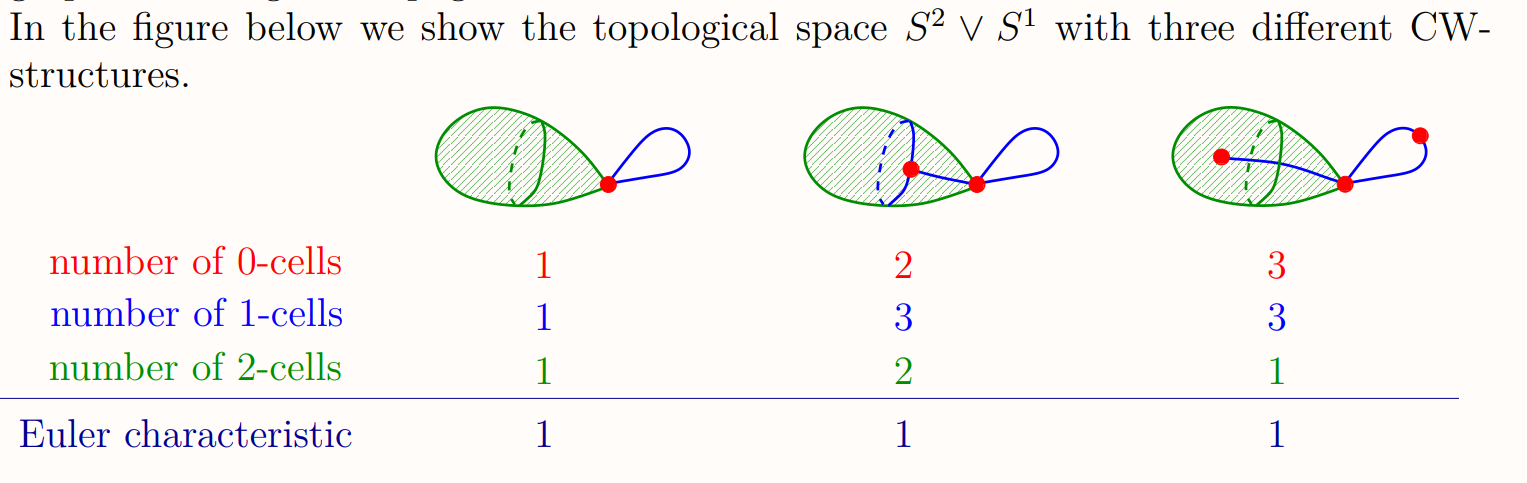
\includegraphics[width=0.8\textwidth]{AT2.png}
						\end{figure}
					\end{center}
				\end{example}
			\subsection{Betti Numbers}
			\subsection{Relative Characteristic}
				\begin{lemma}
					内容...
				\end{lemma}
				\begin{proof}
					内容...
				\end{proof}
			\subsection{Properties}
				\subsubsection{Union}
				\subsubsection{Quotient}
				\subsubsection{Product}
				\subsubsection{Covering}	
					\begin{proposition}
						Let $p:\tilde{X}\rightarrow X$ be a finite covering of a finite path-connected non-empty CW-complex $X$.
						
						We equip $\tilde{X}$ with the structure of a CW-complex given by the CW-complex covering proposition, then
						\begin{gather*}
							\chi(\tilde{X})=[\tilde{X}:X]\cdot \chi(X)
						\end{gather*}
					\end{proposition}
					\begin{proof}
						内容...
					\end{proof}
				\subsection{Calculations of Euler Characteristics}
				\subsection{Applications}
		\section{The Fundamental Theorem of HA}
		\section{The Eilenberg-Zilber Theorem and the Künneth Theorem
		}
	\chapter{Homology}
		According to \textbf{Dold-Kan correspondence} we have
		\begin{gather*}
			Ab^{\Delta_{op}}\Leftrightarrow Ch_{\geq 0}({\mathcal AbD})
		\end{gather*}
		The \textbf{homology groups} of a chain complex of abelian groups are the image under the identification of the homotopy groups and the corresponding $\infty$-groupoids. 
		
		Thus, we have the following \underline{slogan}
		\begin{center}
			Homology=Homotopy,under Dold-Kan Correspondnece
		\end{center}
		\section{Eilenberg-Steenrod Axiom}
		\begin{axiom}
			(Eilenberg-Steenrod) A homology theory $H_*=(H_*,\partial_*)$ with values in $R$-modules is a covariant functor
			\begin{gather*}
				H_*:Top^2\rightarrow \ZZ-grad\quad R-Mod
			\end{gather*}
			Together with a natural transformation $\partial:H_i(X,A)\rightarrow H_{i-1}(A,\varnothing)$ called the \textbf{boundary map} by 
			\begin{gather*}
				\partial_i(X,A):H_i(X,A)\rightarrow H_{i-1}\circ I(X,A)\qquad I:(X,A)\mapsto (A,\varnothing)
			\end{gather*}
			\begin{enumerate}
				\item Homotopy:
				\item Excision:
				\item Dimension:
				\item Additivity:
				\item Exactness:
			\end{enumerate}
		\end{axiom}
		\subsection{}
			\begin{lemma}
				(Exact Sequence of Triples)
			\end{lemma}
			\begin{proof}
				内容...
			\end{proof}
			
			\begin{theorem}
				(Mayer-Vietoris Sequence) Suppose $(X,X_1,X_2)$ be a 
			\end{theorem}
			\begin{proof}
				内容...
			\end{proof}
			
			\begin{corollary}
				(Mayer-Vertoris Sequence for Pushout)
			\end{corollary}
	\chapter{Singular Homology}
		\section{Fundamental}
		
			\subsection{Simplicial Chain Group,Simplicial Homology Group}
			\subsubsection{Simplicial Chain Group}
			\begin{Def}
				Let $X$ be a simplicial complex
				\begin{itemize}
					\item We define the $n$-th simplicial chain group as
					\begin{gather*}
						C_n^{simp}(X):=\{\mbox{Set of all n-chains}\}=\ZZ_2^{\mbox{set of n-simplices of }X}
					\end{gather*}
					\item Define the boundary map
					\begin{gather*}
						\partial_n:C_n^{simp}(X)\rightarrow C_{n-1}^{simp}(X)\\
						\sum a_i\cdot \sigma_i\mapsto \sum a_i\cdot \partial \sigma_i
					\end{gather*}
					\item Sequence:
					\begin{gather*}
						\dots\stackrel{\partial_3}{\rightarrow} C_2^{simp}(X)\stackrel{\partial_2}{\rightarrow} C_1^{simp}(X)\stackrel{\partial_1}{\rightarrow} C_0^{simp}(X)\rightarrow 0
					\end{gather*}
					which is the \textbf{simplicial chain complex} of $X$.
				\end{itemize}
			\end{Def}
			\begin{lemma}
				(Simplicial-Double Boundary Lemma) Let $X$ be a simplicial complex. For every $n\in \NN_0$, the composition
				\begin{gather*}
					0=\partial_n\circ \partial_{n+1}:C_{n+1}^{simp}(X)\rightarrow C_{n-1}^{simp}(X)
				\end{gather*}
			\end{lemma}
			\begin{proof}
				Suppose $\sigma$ be an $(n+1)$-simplex with vertex set $V=\{x_0,\dots,x_{n+1}\}$. We have
				\begin{gather*}
					\partial_n(\partial_{n+1}(\sigma))=\partial_n(\sum_{i=0}^{n+1} Hull(\{x_0,\dots,\hat{x}_i,\dots,x_{n+1}\}))\\
					\qquad=\sum_{i=0}^{n+1}\sum_{j=0,i\not=j}^{n+1} Hull(\{x_0,\dots,\hat{x}_i,\dots,\hat{x}_j,\dots,x_{n+1}\})\\
					\qquad=0
				\end{gather*}
				Because: Each Hull appears twice.
			\end{proof}
			
			\subsubsection{Simplicial Homology Group}
			\begin{Def}
				Let $X$ be a simplicial complex. Furthremore let $n\in \NN$, it follows immediately from above, we have the inclusion
				\begin{gather*}
					im(\partial_{n+1}^{simp}(X)\rightarrow C_n^{simp}(X))\subseteq ker(\partial_n:C_n^{simp}(X)\rightarrow C_{n-1}^{simp}(X))
				\end{gather*}
				Thus, define the $n$-th simplicial homology group as follows:
				\begin{gather*}
					H^{simp}_n(X):Ker(\partial_n)/Im(\partial_{n+1})
				\end{gather*}
			\end{Def}
			\subsection{Examples}
			
			Skip. \url{https://friedl.app.uni-regensburg.de/papers/1t-total-public-october-7-2024.pdf} P2244
		\section{The Singular Homology Groups of a Topolgoical Space}
			\subsection{Review: Algebraic Complex}
				In HA.
				\begin{itemize}
					\item Complex;
					\item Homological Functor;
					\item Operation of Complexes.
				\end{itemize}
			\subsection{The Singular Chain Complex}
				
			\subsection{Singular $n$-Simplex}
			\begin{Def}
				\begin{itemize}
					\item Let $X$ be a topological space and $n\in \NN$. A \textbf{singular $n$-simplex} is a continuous map
					\begin{gather*}
						\sigma?:\Delta^n\rightarrow X
					\end{gather*}
					\item Define the $n$-th singular chain group as follows:
					\begin{gather*}
						C_n(X):=\ZZ(\{\sigma|\sigma\mbox{ is singular n-simplices of }X\})
					\end{gather*}
					\item We refer to an element in $C_n(X)$ as a singular $n$-chain in $X$;
				\end{itemize}
			\end{Def}
			\subsubsection{Face Map}
			\begin{Def}
				Let $n\in \NN$. For $j\in \{0,\dots,n\}$ we define the $j$-th face map as follows
				\begin{gather*}
					i^n_j:\Delta^{n-1}\rightarrow \Delta^n\\
					(t,\dots,t_{n-1})\mapsto (t_0,\dots,t_{j-1},0,\dots,t_{n-1})
				\end{gather*}
			\end{Def}
			\subsubsection{Boundary}
			\begin{Def}
				Let $X$ be a topological space and let $\sigma:\Delta^n\rightarrow X$ be a singular $n$-simplex. 
				
				The \textbf{boundary} $\partial_n \sigma\in C_{n-1}(X)$ is defined as
				\begin{gather*}
					\partial_n \sigma:=\sum_{j=0}^n (-1)^j\cdot \sigma\circ i^n_j
				\end{gather*}
				Then, the map extends uniquely to a linear map
				\begin{gather*}
					\partial_n:C_n(X)\rightarrow C_{n-1}(X)\\
					\sum a_r\cdot \sigma_r\mapsto \sum a_r\cdot \partial \sigma_r
				\end{gather*}
			\end{Def}
			\begin{proposition}
				Let $X$ be a topological space, then the composition
				\begin{gather*}
					\partial_{n-1}\circ \partial_n:C_n(X)\rightarrow C_{n-2}(X)
				\end{gather*}
				is the zero map.
			\end{proposition}
			\begin{proof}
				We have
				\begin{gather*}
					\partial_{n-1}(\partial_n (\sigma))=\partial_{n-1} (\sum_{j=0}^n (-1)^j\cdot \sigma\circ i^n_j)\\
					\qquad=\sum_{k=0}^{n-1}\cdot \sum_{j=0}^n (\sigma\circ i^n_j)\circ i^n_k\\
					=\sum_{0=k<j\leq n} (-1)^{k+j}\cdot \sigma\circ (i^n_j\circ i^{n-1}_k)+\sum_{0=j\leq k\leq n-1} (-1)^{k+j}\cdot \sigma\circ (i^n_j\circ i^{n-1}_k)\\
					=\sum_{0=k<j\leq n}(-1)^{i+j}\cdot \sigma\circ (i^n_j\circ i_k^{n-1})+\sum_{0\leq j\leq k\leq n-1}(-1)^{k+j}\cdot \sigma\circ (i^n_{k+1}\circ i^{n-1}_j)\qquad i^n_j\circ i^{n-1}+k=i^n_{k+1}\circ i_j^{n-1}\\
					=\sum_{0=k<j\leq n}(-1)^{i+j}\cdot \sigma\circ (i^n_j\circ i_k^{n-1})+\sum_{0\leq j\leq k\leq n-1}(-1)^{k+j}\cdot \sigma\circ (i^n_{k+1}\circ i^{n-1}_j)\\
					=0
				\end{gather*}
			\end{proof}
			\subsubsection{Morphisms}
				\begin{Def}
					Let $f:X\rightarrow Y$ be a continuous map between topological spaces. For each $n\in \NN$ we refer to
					\begin{gather*}
						内容...
					\end{gather*}
				\end{Def}
				\begin{lemma}
					($C_*$-Functor Lemma)
				\end{lemma}
				\begin{proof}
					内容...
				\end{proof}
			
			\subsubsection{Path Components}
				\begin{lemma}
					(Path-Component $C_*$-Lemma) Let $X$ be a topological space with path components $\{X_a\}_{a\in A}$. 
					
					Given $a\in A$ we denote by $i_a:X_a\hookrightarrow X$ the inclusion map. The map
					\begin{gather*}
						\oplus_{a\in A} i_a:\oplus_{a\in A} C_*(X_a)\rightarrow C_*(X)
					\end{gather*}
					is an isomorphism of chain complexes.
				\end{lemma}
				\begin{proof}
					内容...
				\end{proof}
				\begin{lemma}
					内容...
				\end{lemma}
				\begin{proof}
					内容...
				\end{proof}
			\subsubsection{Singular Homology Groups}
				\begin{Def}
					Let $X$ 
				\end{Def}
				
				\begin{Def}
					Let $X$ be a topological space:
					\begin{itemize}
						\item 
						\item 
						\item 
					\end{itemize}
				\end{Def}
			\subsubsection{Functor $H_n(-)$}
			\begin{lemma}
				\begin{itemize}
					\item Let $f:X\rightarrow Y$ be a continuous map between topological spaces. The map
					\begin{gather*}
						内容...
					\end{gather*}
					\item $\mathcal Top\rightarrow AbGroup$ defined as followings: 
					\begin{itemize}
						\item 
						\item 
					\end{itemize}
				\end{itemize}
			\end{lemma}
			\begin{proof}
				内容...
			\end{proof}
			\subsection{Calculations of Homology Groups}
				\subsubsection{Empty Spaces}
				\subsubsection{Augment Lemma}
				\subsubsection{Singular $1$-Chain}
		\section{Homology and Homotopies}
			Recall the definitions:
			\begin{itemize}
				\item Homotopy,Homotopy Equivalence;
				\item Chain Homotopy;
			\end{itemize}
			\subsection{Homotopy and Homology Maps} 
			\begin{proposition}
				(Homotopy-$H_*$-Proposition)
			\end{proposition}
			\begin{proof}
				内容...
			\end{proof}
			
			\begin{corollary}
				内容...
			\end{corollary}
			\begin{proof}
				内容...
			\end{proof}
		\section{Exact Sequence, Long Exact Sequences}
			
		\section{Relative Homology}
			\begin{Def}
				Let $(X,A)$ be a pair of topologicalspaces. We view each chain group $C_n(A)$ as a subgroup of $C_n(X)$. Thus we can define
				\begin{gather*}
					C_n(X,A):=C_n(X)/C_n(A)
				\end{gather*}
				and consider the boundary map
				\begin{gather*}
					\partial_n:C_n(X,A)\rightarrow C_{n-1}(X,A)\\
					[c]\mapsto [\partial_n c]
				\end{gather*}
				We refer to
				\begin{gather*}
					\dots\stackrel{\partial_{n+2}}{\rightarrow} C_{n+1}(X,A)\stackrel{n+1}{\rightarrow} C_n(X,A)\stackrel{\partial _n}{\rightarrow}C_{n-1}(X,A)\stackrel{\partial_{n-1}}{\rightarrow} \dots
				\end{gather*}
				And
				\begin{gather*}
					H_n(X,A):=H_n(C_*(X,A))
				\end{gather*}
			\end{Def}
			
			\subsubsection{Functoriality}
			Firstly, take the notion 
			\begin{gather*}
				Ob(PairTop):=\mbox{all pairs of topological spaces}\\
				Mor((X,A),(Y,B)):\{\mbox{all continuous maps }f:X\rightarrow A,f(A)\subseteq B\}
			\end{gather*}
			\begin{Def}
				Let $f:(X,A)\rightarrow (Y,B)$ be a continuous map of pairs of topological spaces. i.e. a continous map
				\begin{gather*}
					f:X\rightarrow Y\qquad f(A)\subseteq B
				\end{gather*}
				It followsthat: There exists a chain map
				\begin{gather*}
					f_*:C_n(X,A)\rightarrow C_n(Y,B)\\
					H_n(f_*):H_n(X,A)\rightarrow H_n(Y,B)
				\end{gather*}
			\end{Def}
			\begin{lemma}
				(Relative-$H_*$-Functor Lemma) The maps
				\begin{gather*}
					(X,A)\mapsto (C_*(X,A),\partial_*)\\
					(f:(X,A)\rightarrow (Y,B))\mapsto (f_*:C_*(X,A)\rightarrow C_*(Y,B))
				\end{gather*}
				define a covariant functor from the subcategory $\mathcal PairTop$ of pairs of topological spaces to the category $\mathcal ChCplx$ of chain complexes and for each $n\in \NN$,
				\begin{gather*}
					(X,A)\rightarrow H_n(X,A)\\
					(f:(X,A)\rightarrow (Y,B))\mapsto (f_*:H_n(X,A)\rightarrow H_n(Y,B))
				\end{gather*}
			\end{lemma}
			\begin{proof}
				Immediately from the defifnition.
			\end{proof}
		
			
			\subsection{Long Exact Sequence of a Triple}
			\subsubsection{The Triple of Topological spaces}
			\begin{Def}
				\begin{itemize}
					\item A \textbf{triple of topological space} is a triple $(X,B,A)$ where $X$ is a topological space and $A\subseteq B\subseteq X$ are subspaces;
					\item Morphisms $f:(X,B,A)\rightarrow (X',B',A')$ such that
					\begin{gather*}
						f:X\rightarrow X',f(B)\subseteq B',f(A)\subseteq A'
					\end{gather*}
				\end{itemize}
			\end{Def}
			\begin{proposition}
				(LES of Triple Propositions)
			\end{proposition}
			\begin{proof}
				内容...
			\end{proof}
			\subsection{Relative Homology Groups and Homotopies}
	
			\begin{proposition}
				Let $f,g:(X,A)\rightarrow (Y,B)$ be two continuous maps betwween pairs of topological sapces. If $f,g$ are homotopic, then the chain maps
				\begin{gather*}
					f_*,g_*:C_*(X,A)\rightarrow C_*(Y,B)
				\end{gather*}
				are chain homotopic. In particular for every $n\in \NN$ we have
				\begin{gather*}
					f_*=g_*:H_n(X,A)\rightarrow H_n(Y,B)
				\end{gather*}
			\end{proposition}
			\begin{proof}
				内容...
			\end{proof}
				\begin{proposition}
				(LES-of-Triple Proposition) Let $X$ be a topological space and let $A\subseteq B\subseteq X$ be two subspaces. Let $i:(B,A)\rightarrow (X,A)$ and by $p:(X,A)\rightarrow (X,B)$ be the obvious maps
				\begin{itemize}
					\item For each $n\in \NN$, the following map is a well-define group homomorphism
					\begin{gather*}
						\partial_n:H_n(X,B)\rightarrow H_{n-1}(B,A)\\
						[\sum s_j\cdot (\sigma_j:\Delta^n\rightarrow X)]\mapsto [\sum_{j=1}^k s_j\cdot \partial \sigma_j]
					\end{gather*}
					We refer $\partial_n$ as a \textbf{connecting homomorphism} of the triple $(X,B,A)$.
					\item The connecting homomorphsim are natural: In particular, for any continuous map
					\begin{gather*}
						f:(X,A,B)\rightarrow (\hat{X},\hat{A},\hat{B})
					\end{gather*}
					of triples of topological spaces the following diagram commutes:
					\begin{center}
						\begin{tikzcd}
							\dots\arrow[r]&H_n(B,A)\arrow[d]\arrow[r]&H_n(X,A)\arrow[r]\arrow[d]&H_n(X,B)\arrow[r]\arrow[d]&H_{n-1}(B,A)\arrow[r]\arrow[d]&\dots\\
							\dots\arrow[r]&H_n(\hat{B},\hat{A})\arrow[r]&H_n(\hat{X},\hat{A})\arrow[r]&H_n(\hat{X},\hat{B})\arrow[r]&H_{n-1}(\hat{B},\hat{A})\arrow[r]&\dots
						\end{tikzcd}
					\end{center}
					\item The maps
					\begin{center}
						\begin{tikzcd}
							\dots\arrow[r]&H_n(B,A)\arrow[r]&H_n(X,A)\arrow[r]&H_n(X,B)\arrow[r]&H_{n-1}(B,A)\arrow[r]&\dots
						\end{tikzcd}
					\end{center}
					form an exact squence, called \textbf{long exact sequence} of the triple $(X,B,A)$.
				\end{itemize}
			\end{proposition}
			\begin{proof}
				Firstly, we should prove the exactness of 
				\begin{center}
					\begin{tikzcd}
						0\arrow[r]&C_*(B,A)\arrow[r]&C_*(X,A)\arrow[r]&C_*(X,B)\arrow[r]&0
					\end{tikzcd}
				\end{center}
				Immedaitely from the definition. 
				
				Then: Suppose $z\in H_n(X,B)$ with $z=[\sum s_j\cdot (\sigma_j:\Delta^n\rightarrow X)]$
				
				Or: Notice that (depends on snake lemma) we have
				\begin{gather*}
					0\rightarrow Ker(d^{C_*(B,A)}_n)\rightarrow Ker(d^{C_*(X,A)}_n)\rightarrow Ker(d^{C_*(X,B)}_n)\stackrel{\delta}{\rightarrow} Coker(d^{C_*(B,A)}_n)\rightarrow Coker(d^{C_*(X,A)}_n)\rightarrow Coker(d^{C_*(X,B)}_n)\rightarrow 0
				\end{gather*}
				Then, for $\delta$, consider the following square
				\begin{center}
					\begin{tikzcd}
					&	Ker(d^{C_*(B,A)}_n)\arrow[r]\arrow[d]&Ker(d^{C_*(X,A)}_n)\arrow[d]\arrow[r]&Ker(d^{C_*(X,B)}_n)\arrow[d]\\
						0\arrow[r]&C_n(B,A)\arrow[d]\arrow[r]&C_n(X,A)\arrow[r]\arrow[d]&C_n(X,B)\arrow[r]\arrow[d]&0\\
						0\arrow[r]&C_{n-1}(B,A)\arrow[r]\arrow[d]&C_{n-1}(X,A)\arrow[r]\arrow[d]&C_{n-1}(X,B)\arrow[d]\arrow[r]&0\\
						&Coker(d^{C_*(B,A)}_n)\arrow[r]&Coker(d^{C_*(X,A)}_n)\arrow[r]&Ker(d^{C_*(X,B)}_n)
					\end{tikzcd}
				\end{center}
				Diagram chasing: Suppose $c\in Ker(d_n^{C_*(X,B)})\subseteq C_n(X,B)$. We have 
				\begin{gather*}
					p_*(b)=,b\in Ker(d_n^{C_n(X,A)})\subseteq C_n(X,A)\\
					i_*(a)=d(b)
				\end{gather*}
				And notice that $a\in ker(d_{n-1})$. Because of $C_n(B,A)\rightarrow C_n(X,A)\rightarrow C_{n-1}(X,A)$ maps $a$ to $0$. Now consider the square $C_{n-1}(B,A)\rightarrow C_{n-2}(B,A)\rightarrow C_{n-2}(X,A)$.
			\end{proof}
			
			\begin{proposition}
				(LES-of-Pair Proposition)
				\begin{itemize}
					\item Let $X$ be a topological space and $B\subseteq X$ be a subspace. The connecting homomorphism of the LES-of-Triple proposition applied to $A=\varnothing$ gives rise to an exact seuqence
					\begin{gather*}
						内容...
					\end{gather*}
					\item The connecting homomorphism is natural. In particular, given a continuous map
					\begin{gather*}
						f:(X,A)\rightarrow (Y,B)
					\end{gather*}
					between pairs of topological spaces we obtain a commutative
					\begin{center}
						\begin{tikzcd}
							&H_n(A)&
						\end{tikzcd}
					\end{center}
				\end{itemize}
			\end{proposition}
			\begin{proof}
				内容...
			\end{proof}
			
			\begin{corollary}
				(Homotopy Equivalence-Relative-$H_*$-Corollary) 
			\end{corollary}
			\begin{proof}
				内容...
			\end{proof}
			
			\begin{corollary}
				(Deformation Retract-Relative $H_*$-Corollary) Let $X$ be a topological space.If $A\subseteq X$ is a deformation retract of $X$, then
				\begin{gather*}
					H_n(X,A)=0,n\in \NN
				\end{gather*}
			\end{corollary}
			\begin{proof}
				内容...
			\end{proof}
			\subsection{Relative Homology Groups and Homotopies}
			\begin{proposition}
				Let $f,g:(X,A)\rightarrow (Y,B)$ be two continuous maps between pairs of topological spaces. If $f,g$ homotopic, then the chain maps
				\begin{gather*}
					f_*,g_*:C_*(X,A)\rightarrow C_*(Y,B)
				\end{gather*}
				are chain homotopic, in particular for every $n\in \NN$ we have
				\begin{gather*}
					f_*=g_*:H_n(X,A)\rightarrow H_n(Y,B)
				\end{gather*}
				Let $f,g:(X,A)\rightarrow (Y,B)$ be two continuous maps between pairs of topological spaces and let
				\begin{gather*}
					内容...
				\end{gather*}
			\end{proposition}
			\begin{proof}
				内容...
			\end{proof}
			\subsection{Excision}
				\begin{proposition}
					Let $X$ be a topological space, $A\subseteq X$ open and $Z\subseteq A$ closed, with
					\begin{gather*}
						Z\subseteq A
					\end{gather*}
					The inclusion $(X-Z,A-Z)\rightarrow (X,A)$ induces an epimorphism
					\begin{gather*}
						H_1(X-Z,A-Z)\rightarrow H_1(X,A)
					\end{gather*}
				\end{proposition}
				\begin{proof}
					内容...
				\end{proof}
			\subsection{Retract}
			\begin{proposition}
				Let $(X,A)$ be a pair of topological spaces. If $A$ is a retract of $X$, i.e. exists $f:X\rightarrow A$ such that
				\begin{gather*}
					f\circ \iota_A=f|A=id_A
				\end{gather*}
				then for each $n\in \NN$, there exists an isomorphism
				\begin{gather*}
					H_n(X)\cong H_n(A)\oplus H_n(X,A)
				\end{gather*}
			\end{proposition}
			\begin{proof}
				内容...
			\end{proof}
		\section{Reduced Homology}
			\begin{Def}
				Let $X$ be a toplogical space. Then we know that the following is a generalized chain complex
				\begin{gather*}
					\dots\stackrel{\partial_2}{\rightarrow} C_1(X)\stackrel{\partial_1}{\rightarrow} C_0(X)\stackrel{\epsilon_X}{\rightarrow} \ZZ\rightarrow 0
				\end{gather*}
				By $\epsilon_X:\sum r_i\cdot \sigma_i\mapsto \sum r_i$
				
				We introduce the following definitions:
				\begin{itemize}
					\item We refer to this chain complex as the augmented chain complex $\hat{C}_*(X)$ of $X$;
					\item Given $n\in \ZZ_{\geq -1}$ we refer to
					\begin{gather*}
						\hat{H}_n(X):=H_n(\hat{C}_*(X))
					\end{gather*}
				\end{itemize}
			\end{Def}
			\begin{lemma}
				内容...
			\end{lemma}
			\begin{proof}
				内容...
			\end{proof}
		\section{The Excision Theorem}
			\begin{theorem}
				(Excision Theorem) Let $X$ be a topological space and let $Z\subseteq A\subseteq X$ be subsets. If the closure of $Z$ is contained in the interior of $A$ then the inclusion
				\begin{gather*}
					(X-Z,A-Z)\rightarrow (X,A)
				\end{gather*}
				induces for each $n\in \NN$ an isomorphism
				\begin{gather*}
					H_n(X-Z,A-Z)\rightarrow H_n(X,A)
				\end{gather*}
			\end{theorem}
			\begin{proof}
				内容...
			\end{proof}
			\begin{theorem}
				(The Excision Theorem) Let $X$ be topological space, $K$ be a subset of $X$ and $U$ be a neighborhoo of the closure of $K$. Then, the inclusion $(U,U-K)\rightarrow (X,X-K)$ induces for each $n\in \NN$ an isomorphism
				\begin{gather*}
					H_n(U,U-K)\rightarrow H_n(X,X-K)
				\end{gather*}
			\end{theorem}
				\subsubsection{Suspensions and Homology Groups}
					\begin{Def}
						Let $X$ be a non-empty  topological space;
						\begin{itemize}
							\item Define the \textbf{suspension} of $X$ to be the topological space
							\begin{gather*}
								\Sigma(X):=(X\times [-1,1])/(X\times \{-1\})/(X\times \{1\})
							\end{gather*} 
							\item Define:
							\begin{itemize}
								\item North Pole $N=[X\times \{1\}]$;
								\item South Pole $S=[X\times \{-1\}]$;
							\end{itemize}
							\item Set:
							\begin{gather*}
								C_-X:=\Sigma(X)-\{N\}\qquad C_+X:=\Sigma(X)-\{S\}
							\end{gather*}
							\item Given a continuous map $f:X\rightarrow Y$ between topological spaces, then 
							\begin{gather*}
								\Sigma(f):\Sigma(X)\rightarrow \Sigma(Y)\\
								[(x,t)]\mapsto [(f(x),t)]
							\end{gather*}
						\end{itemize}
					\end{Def}
					
					\begin{proposition}
						(Suspension-$H_*$-Proposition)
					\end{proposition}
					\begin{proof}
						内容...
					\end{proof}
					
					\begin{proposition}
						(Reflection-on-Suspension-$H_*$-Proposition)
						Let
						\begin{gather*}
							\rho:\Sigma(X)\rightarrow \Sigma(X)\\
							[(x,t)]\mapsto [(x,-t)]
						\end{gather*}
						be the natural reflection. For any $k\in \NN$, the induced map
						\begin{gather*}
							\rho_k:\hat{H}_k(\Sigma(X))\rightarrow \hat{H}_k(\Sigma(X))
						\end{gather*}
						given by multiplication by $-1$.
					\end{proposition}
					\begin{proof}
						内容...
					\end{proof}
					\subsubsection{Homology Group of Sphere}
					\subsubsection{Brouwer's Fixed Point Theorem}
					\subsubsection{Homology Group of Wedge}
					\subsubsection{The Long Exact Sequence for Quotients}
		\section{Local Homology}
			\subsection{Generator of $H_n(\Delta^n,\partial \Delta^n)$}
			
			\begin{lemma}
				内容...
			\end{lemma}
			\begin{proof}
				内容...
			\end{proof}
			\subsection{Local Homology Groups of a Topological Space}
				\begin{Def}
					内容...
				\end{Def}
		\section{Homology and Self-Maps of Spheres}
			\subsection{The Degree}
				\begin{Def}
					Let $(G,+)$ be a group such that $G$,$\Phi:G\rightarrow G$ be a homomorphism.
				
					Note that $\Phi$ is given by multiplication by a unique integer which we refer to as the degree $deg(\Phi)$.
				\end{Def}
				
				\begin{lemma}
					(Algebraic Degree Lemma) Let $(G,+)$ be a group that is isomorphic to $\ZZ$:
					\begin{itemize}
						\item Let $g\in G$ be any non-trivial element. Furthermore let $\Phi:G\rightarrow G$ be a homomorphism. The degree $deg(\Phi)$ is uniquely determined by the quality
						\begin{gather*}
							\Phi(g)=deg(\Phi)\cdot g
						\end{gather*}
						\item Let $\varphi:G\rightarrow H$ be an isomorphism and let $f:H\rightarrow H$ be a homomorphism. Then,
						\begin{gather*}
							deg(\varphi^{-1}\circ f\circ \varphi:G\rightarrow G)=deg(f:H\rightarrow H)
						\end{gather*}
					\end{itemize}
				\end{lemma}
				\begin{proof}
					内容...
				\end{proof}
				\subsubsection{Sphere-Degree}
				\begin{lemma}
					(Sphere-Degree Lemma) Let $n\in \NN$ and $f,g:S^n\rightarrow S^n$ be two continuus maps:
					\begin{itemize}
						\item $deg(id_{S^n})$;
						\item If $f$ is not surjective, then $deg(f)=0$;
						\item If $f$ is homotopic to $g$, then $deg(f)=deg(g)$;
						\item $deg(f\circ g)=deg(f)\cdot deg(g)$;
						\item If $f$ is a self-homeomorphism of $S^n$, then $deg*f^{-1}=deg(f)$.
					\end{itemize}
				\end{lemma}
				\begin{proof}
					内容...
				\end{proof}
				
				\begin{lemma}
					(Degree-of-Power Lemma) Given $k\in \ZZ$ we have
					\begin{gather*}
						内容...
					\end{gather*}
				\end{lemma}
				\begin{proof}
					内容...
				\end{proof}
				
				\begin{lemma}
					(Sphere-Degree-Matrix Lemma) Given any $A\in O(n+1)$ we have
					\begin{gather*}
						内容...
					\end{gather*}
				\end{lemma}
				\begin{proof}
					内容...
				\end{proof}
				\subsubsection{Suspension}
				\begin{lemma}
					内容...
				\end{lemma}
				\begin{proof}
					内容...
				\end{proof}
				
			\subsection{The Hairy Ball Theorem}
				\begin{theorem}
					(Sphere-Degree Fiexed Point Theorem) Let $f:S^n\rightarrow S^n$ be a continuous map. If 
					\begin{gather*}
						内容...
					\end{gather*}
				\end{theorem}
				\begin{proof}
					内容...
				\end{proof}
				
				\begin{proposition}
					内容...
				\end{proposition}
				\begin{proof}
					内容...
				\end{proof}
				
				\begin{theorem}
					（airyB阿拉蕾Theo'r'me'm
				\end{theorem}
				\begin{proof}
					内容...
				\end{proof}
			\subsection{Local Degrees of Self-Maps of Spheres}
				\begin{Def}
					Let $f:M\rightarrow N$ be a continuous map between two oriented $n$-dimensional smooth manifolds, $x\in M-\partial M$. 
					
					If $f$ is a local diffeomorphism, then define the \textbf{local degree} at point $x$:
					\begin{gather*}
						内容...
					\end{gather*}
				\end{Def}
		\section{Mayer-Vietoris Sequence}
		\begin{lemma}
			(Brratt-Whitehead,Algebraic) Consider the following commutative diagram of homomorphisms between abelian groups
			\begin{center}
				\begin{tikzcd}
					\dots&C_n'&C_n&C_n''&C_{n-1}'&\dots\\
					\dots&D_n'&D_n&d_N''&D_{n-1}'&\dots
				\end{tikzcd}
			\end{center}
			Then, define
			\begin{gather*}
				\Delta_n:=\partial_n\circ (f''_n)^{-1}\circ q_n:D_n\rightarrow C_{n-1}'
			\end{gather*}
			The following sequence is exact
			\begin{gather*}
				\dots\rightarrow C_n'\stackrel{(i_n,-f_n')}{\rightarrow} C_n\oplus D_n'\stackrel{f_n\oplus j_n}{\rightarrow} D_n\stackrel{\Delta_n}{\rightarrow} C_{n-1}'\rightarrow\dots
			\end{gather*}
		\end{lemma}
		\begin{proof}
			内容...
		\end{proof}
		\begin{theorem}
			(Mayer-Vietoris) Let $X$ be a topological space and let $A,B\subseteq X$ be subspaces such that one of the following three conditions holds:
			\begin{itemize}
				\item $X$ is the union of the interiors of $A$ and $B$. i.e.
				\begin{gather*}
					X=\mathring{A}\cup \mathring{B}
				\end{gather*}
				\item $X$ is a CW-complex and $A,B$ are subcomplexes with $X=A\cup B$;
				\item $X$ is a topological manifold and $A,B\subseteq X$ are two codimension-zero manifolds such that the following conditions are satisfied:
				\begin{itemize}
					\item $X=A\cup B$;
					\item $A\cap B$ is a union of components of $\partial A$ and it is a union of components of $\partial B$;
					\item $A$ and $B$ are closed subsets of $X$;
				\end{itemize}
			\end{itemize}
			Then, by excision theorem; the CW-excision theorem; Manifold excision theorem each induced by
			\begin{gather*}
				i_{(A,A\cap B)}^{(X,B)}:H_A(A,A\cap B)\rightarrow H_n(X,B)
			\end{gather*}
			is an isomorphism. We refer to the homomorphism
			\begin{gather*}
				H_n(X)\stackrel{}{\rightarrow} H_n(X,B)\stackrel{}{\rightarrow} H_n(A,A\cap B)\stackrel{\partial_n}{
				\rightarrow} H_{n-1}(A\cap B)
			\end{gather*}
			as the connecting homomorphism\begin{gather*}
				\partial_n:H_n(X)\rightarrow H_{n-1}(A\cap B)
			\end{gather*}
			corresponding to $(X,A,B)$. The connecting homomorphism is natural in a suitable sense and with the notation the following sequence is exact:
			\begin{gather*}
				\dots\rightarrow H_n(A\cap B)\stackrel{}{\rightarrow} H_n(A)\oplus H_n(B)\stackrel{}{\rightarrow} H_n(X)\stackrel{}{}H_{n-1}(A\cap B)\rightarrow \dots
			\end{gather*}
			Totally analogous statement also hold if we replace the homlogy groups of $A\cap B,A,B,X$ by corresponding reduced homology groups.
		\end{theorem}
		\begin{proof}
			内容...
		\end{proof}
		Another Proof:
		\begin{gather*}
			内容...
		\end{gather*}
		
		\begin{Def}
			The long exact sequence of above is called \textbf{Mayer-Vietoris Sequence of the decomposition} $X=A\cup B$.
		\end{Def}
		\subsection{Applications}
			\subsubsection{Suspension}
			\begin{proposition}
				(Suspension-$H_*$-Proposition) Given any topological space $X$ and given any $k\in \ZZ$ we have a natural isomorphism
				\begin{gather*}
					\Sigma_X:\hat{H}_{k+1}(\Sigma(X))\stackrel{\cong}{\rightarrow} H_k(X)
				\end{gather*}
			\end{proposition}
			\begin{proof}
				内容...
			\end{proof}
			
			\subsubsection{Mapping Torus}
			\begin{Def}
				Let $X$ be a topological space and $f:X\rightarrow X$ be a continuous map. We refer to
				\begin{gather*}
					Tor(X,f):=(X\times [0,1])/(x,0)\sim (f(x),1)
				\end{gather*}
			\end{Def}
			Especially, 
			\begin{gather*}
				\Phi:Tor(X,id)\rightarrow X\times S^1\\
				[(x,t)]\mapsto (x,exp(2\pi it))
			\end{gather*}
			is an isomorphism.
			
			\begin{example}
				(Mobius Band) $X=[-1,1]$
			\end{example}
			
			\begin{proposition}
				(Mapping Torus $H_*$-Proposition) Let $X$ be a topological space, $f:X\rightarrow X$ be a continuous map. Then, denote
				\begin{gather*}
					i:X\rightarrow Tor(X,f)\qquad x\mapsto [(x,0)]
				\end{gather*}
				for every $n\in \NN$, there exists a natural homomorphism 
				\begin{gather*}
					\partial_n:H_n(Tor(X,f))\rightarrow H_{n-1}(X)
				\end{gather*}
				such that the following sequence is exact:
				\begin{gather*}
					\dots\rightarrow H_n(X)\stackrel{f_*-id}{\rightarrow} H_n(X)\stackrel{i_*}{\rightarrow} H_n(Tor(X,f))\stackrel{\partial_n}{\rightarrow} H_{n-1}(X)\rightarrow \dots
				\end{gather*}
			\end{proposition}
			\begin{proof}
				内容...
			\end{proof}
			
			\subsection{Homology and Cell Attachments}
			\begin{proposition}
				内容...
			\end{proposition}
		\section{Homology Groups and Direct Limits}
		\section{Cellular Homology}
			\begin{lemma}
				(Skeleton-$H_*$-Lemma) Let $X$ be a CW-complex and $n\in \NN$,
				\begin{itemize}
					\item 
					\item 
					\item 
					\item 
				\end{itemize}
			\end{lemma}
			\begin{proof}
				内容...
			\end{proof}
			\subsection{Definitions}

		\section{The Euler Characteristic}
			\begin{Def}
				Define:
				\begin{gather*}
					\chi(X):=\sum_{n\in \NN} (-1)
				\end{gather*}
			\end{Def}
			\subsection{The Euler Characteristic of CW-Complex}
				\begin{proposition}
					(Homology-$\chi$-Proposition) Given any finite CW-complex $X$ we have
					\begin{gather*}
						内容...
					\end{gather*}
				\end{proposition}
				\begin{proof}
					内容...
				\end{proof}
				
				\begin{corollary}
					(Homotopy Type $\chi$-Corollart)
				\end{corollary}
				\begin{proof}
					内容...
				\end{proof}
			\subsection{Betti Number}
				\begin{Def}
					Let $(X,A)$ be a pair:
					\begin{itemize}
						\item Define the \textbf{Betti number} of $(X,A)$ to be
						\begin{gather*}
							b_n(X,A):=rank(H_n(X,A))
						\end{gather*}
						\item If $\sum_{n\in \NN} b_n(X,A)$ is finite, then define the \textbf{Euler characteristic} of $(X,A)$ to be
						\begin{gather*}
							\chi(X,A):=\sum_{n} (-1)^n\cdot b_n(X,A)
						\end{gather*}
					\end{itemize}
				\end{Def}
				
				\begin{lemma}
					(Relative-$\chi$-Lemma)
				\end{lemma}
				\begin{proof}
					内容...
				\end{proof}
			\subsection{Calculation of Euler Characteristics}
			\subsection{Applications}
				\subsubsection{Euler's Formula}
		\section{The Hurewicz Theorem}
		\section{Jordan-Brouwer Separation Theorem}
		\section{Moore Space}
			\begin{Def}
				内容...
			\end{Def}
	\chapter{Localization}
	\chapter{Note}
		\section{4/15} 
			\begin{itemize}
				\item Review: Homology
				\item Definition: Cochain,Cohomology,morphisms,
				\item Cochain homotopy $f,g:C\rightarrow D$
				\begin{gather*}
					s^n:C^n\rightarrow D^{n-1}\qquad d^{n-1}\circ s^n+s^{n+1}\circ d^n=f^n-g^n
				\end{gather*}
				\item Functor
				\begin{gather*}
					D:(C^n)\mapsto \qquad {\mathcal Coch}(A)\rightarrow {\mathcal Ch}(A)
				\end{gather*}
				\begin{proposition}
					\begin{gather*}
						H^n(DC)=H_{-n}(C)
					\end{gather*}
				\end{proposition}
				\begin{proof}
					内容...
				\end{proof}
				\begin{proposition}
					(Commutes with $H^n$ functor) $(H^nf)([x])=[f^n(x)]$
				\end{proposition}
				\item Meaning of cochain homotopy: Induces the same map on $H^n$;
				\item Long exact sequence $\rightarrow H_n(A)\rightarrow\dots\rightarrow H_n(C)\stackrel{\partial}{\rightarrow} H^{n+1}(A)\rightarrow\dots,\partial [x]=[y],f^{n+1}$
				\item Consider $Hom(-,A)$ has an inverse direction of chain complex. 
				\begin{gather*}
					d^n:Hom(C,A)^n\rightarrow H_n(C,A)^{n+1}\\
					f\mapsto f\circ d_{n+1}
				\end{gather*} 
				$Hom(-,A)$ Contravariant functor $Ch(\mathcal{A})\rightarrow {\mathcal Ab}$.
				\item \begin{gather*}
					H^n(Y,A):=H^n(Hom(C(Y,\ZZ),A))
				\end{gather*}
				Relative $Y'\subseteq Y$
				\begin{gather*}
					H^n(Y,Y',A):=H^n(Hom(\frac{C(Y,\ZZ)}{C(Y',\ZZ)}),A)
				\end{gather*}
				\item X space, $X'\subseteq X$(especially, $X'=\varnothing$)
				\begin{gather*}
					H^n(X,X',A):=H^n(S(X),S(X'),A)
				\end{gather*}
				\item We have
				\begin{gather*}
					Hom(C_n(Y,\ZZ),A)^n=\prod_{Y_n} A
				\end{gather*}
				\item $Y'\subseteq Y$ subsimplicial set,
				\begin{gather*}
					Hom(\frac{C_*(Y,\ZZ)}{C_*(Y',\ZZ)},A)_n=Hom(\frac{C_n(Y,\ZZ)}{C_n(Y',\ZZ)},A)=Hom(\frac{\pi(Y_n)}{\pi(Y_n')},A)=\{f\}
				\end{gather*}
				Thus, exact
				\begin{gather*}
					0\rightarrow Hom(\frac{C_*(Y,\ZZ)}{C_*(Y',\ZZ)},A)\rightarrow 
				\end{gather*}
				\item Homotopy-Invariance
				\begin{proposition}
					If $f,g:X\rightarrow Y$ homotopy chain map, then $H^n(f;A)=H^n(g;A):H_n(X;A)\rightarrow H_n(Y;A)$.
				\end{proposition}
				\item \begin{example}
					内容...
				\end{example}
				\item Warning $Hom(-,A)$ may not generally sends q-i to q-i
				\begin{example}
					\begin{tikzcd}
						\dots&0&\ZZ&\ZZ&0&\dots\\
						\dots&0&0&\ZZ/2&0&\dots
					\end{tikzcd}
				\end{example}
				\item Review: (Whitehead)For chain complex every quasi-isomorphhism $C\stackrel{\delta}{\rightarrow} D$ be dege map free chain complex is a chain homotopy equivalence.
				\item Consider excoi triple $(U\subseteq Y\subseteq X,\bar{U}\subseteq \o{Y})$. $Hom(-,A)$ is a q-i for the admisiible cone $X=(X-U)\cup Y$ the
				\begin{gather*}
					H^n(X-Y,Y-Y,A)\cong H^n(X;Y;A)
				\end{gather*}
				\item $H^m(S^n,A)=\begin{cases}
					A\oplus A&m=n\\
					A&\\
					0&else
				\end{cases},H^m(D^n,S^n,A)=$
				\item Cellular cochain complex:
				$X$ CW-Complex, A ab group
				\begin{Def}
					$C_{cell}^*(X,A)=Hom(C_*^{cell}(X,\ZZ),A)$
				\end{Def}
				See: $C_n^{cell}(X,\ZZ)=H_n(X_n,X_{n-1},\ZZ)$, $C^n_{cell}(X,A)=H^n(X_n,X_{n-1},A)$
				\item Natural isomorphism
				\begin{gather*}
					H^*(C^*_{cell}(X,A))\cong H^n(X,A)
				\end{gather*}
				\begin{example}
					$\CC P^n$.
				\end{example}
			\end{itemize}
		\chapter{Simplicial Cohomology}
			\section{Chirality}
				\begin{Def}
					内容...
				\end{Def}
				\subsection{Hyperplane-Reflection}
					\begin{lemma}
						内容...
					\end{lemma}
			\section{Cochain Complexes and Dual Complexes}
				\subsection{Preparations}
				\subsubsection{The Hom-Functor}
					Consider
					\begin{gather*}
						Hon(-,X)\qquad f:A\rightarrow B\Rightarrow f^*:Hom(B,G)\rightarrow Hom(A,G)
					\end{gather*}
					\begin{lemma}
						\begin{itemize}
							\item Given an abelian group $G$, the map $A\mapsto Hom(A,G),(f:A\rightarrow B)\mapsto (f^*:Hom(B,G)\rightarrow Hom(A,G))$
							\item If $R$ is a commutative ring, then the above maps
							\begin{gather*}
								A\mapsto Hom(A,R)\qquad f\mapsto f^*
							\end{gather*}
							defines a contravariant functor from the category grooups to $Mod_R$.
						\end{itemize}
					\end{lemma}
					\begin{proof}
						Omitted.
					\end{proof}
					
					\begin{lemma}
						内容...
					\end{lemma}
					\begin{proof}
						内容...
					\end{proof}
				\subsubsection{Cochain Complexes}
				\subsubsection{Cochain Maps}
				
					
					
				\subsection{Calculation of Some Cohomology}
					\subsubsection{Empty Space}
					\subsubsection{Path Component $H^*$-Lemma}
					\subsubsection{title}
					\subsubsection{title}
				\subsection{Basic Properties of Cohomology Groups}
				\subsection{Reduced Cohomology Groups}
				
			\section{The Cohomology Group of Topological Spaces}
				\subsection{Singular Cohomology Groups}
				\begin{Def}
					Let $(X,A)$ be a pair of topological spaces, and let $G$ be an abelian group.
					\begin{itemize}
						\item For each $n\in \NN$, write
						\begin{gather*}
							C^n(X,A;G):=Hom(C_n(X,A),G)\qquad \delta_n:=\partial_{n+1}^*:C^n(X,A;G)\rightarrow C^{n+1}(X,A;G)
						\end{gather*}
						We use the following notations:
						\begin{itemize}
							\item $C^n(X,A;G)$ is called the \textbf{singular $n$-cochain}. 
							\item The kernel of 
							\begin{gather*}
								\delta_n:C^n(X,A;G)\rightarrow C^{n+1}(X,A;G)
							\end{gather*}
							as \textbf{singular $n$-cocyles}.
							\item The image of 
							\begin{gather*}
								\delta_n:C^n(X,A;G)\rightarrow C^{n+1}(X,A;G)
							\end{gather*}
							as \textbf{singluar $n$-coboundaries}.
						\end{itemize}
						\item Define the cochain complex
						\begin{gather*}
							\dots\leftarrow C^{n+1}(X,A;G)\stackrel{\delta_n}{\leftarrow} C^n(X,A;G)\stackrel{\delta_{n-1}}{\leftarrow} \dots\stackrel{\delta_0}{\leftarrow} C^0(X,A;G)\leftarrow 0
						\end{gather*}
						the cohoomology groups
						\begin{gather*}
							H^n(X,A;G):=ker(\delta_n)/im(\delta_{n-1})
						\end{gather*}
						\item Especially, $A=\emptyset,C^n(X;G):=C^n(X,\emptyset;G)$.
					\end{itemize}
				\end{Def}
				\subsubsection{Morphisms induced by Continuous Maps}
				\begin{Def}
					Consider a continuous map
					\begin{gather*}
						f:(X,A)\rightarrow (Y,B)
					\end{gather*}
					
					Then, the induced map
					\begin{gather*}
						f^*:C^*(Y,B;G)\rightarrow C^*(X,A;G)
					\end{gather*}
					And the group homomorphism
					\begin{gather*}
						f^*:H^n(Y,B;G)\rightarrow H^n(X,A;G)
					\end{gather*}
				\end{Def}
				\begin{lemma}
					内容...
				\end{lemma}
				\begin{proof}
					内容...
				\end{proof}
					
					\subsection{Example:Explicit Cochains and Cocycles}
					\subsubsection{Circles}
						Consider the topological space $X=S^1$. with
						\begin{gather*}
							p:\RR\rightarrow S^1\qquad t\mapsto exp(2\pi it)
						\end{gather*}
						be the universal covering of $S^1$. Then, let 
						\begin{gather*}
							\sigma^1:\Delta^1\rightarrow S^1
						\end{gather*}
						be singular 1-simplex. $\Delta^1$ is simply connected, by the covering existence theorem
						\begin{gather*}
							内容...
						\end{gather*}
						\begin{lemma}
							($\theta$-Cocycle Lemma) 
							\begin{itemize}
								\item 
								\item 
							\end{itemize}
						\end{lemma}
					\subsubsection{title}
			\section{Cellular Cohomology and the Kronecker Pairing}
				\subsection{Cellular Cohomology}
					
				\subsubsection{Review: Cellular Cohomology}
					\begin{Def}
						Let $X$ be a CW-complex:
						\begin{itemize}
							\item Denote $X^n$ the $n$-skeleton
							\item Write
							\begin{gather*}
								C^{CW}_n(X):=H_n(X^n,X^{n-1})
							\end{gather*}
							We refer to the elements of $C^{CW}_n(X)$ as \textbf{cellular chain}.
							\item \begin{itemize}
								\item 
								\item 
							\end{itemize}
							\item We denoted by
							\begin{gather*}
								d_n:C_n^{CW}(X)\rightarrow C_{n-1}^{CW}(X)
							\end{gather*}
							the cellular boundary map.
							\item 
							\item 
						\end{itemize}
					\end{Def}
					
					\begin{Def}
						(Cellular Cohomology) Let $X$ be a CW-complex, $G$ an abelian group:
						\begin{itemize}
							\item Let $n\in \NN$:
							\begin{itemize}
								\item We refer to elements of $Hom(C^{CW}_n(X),G)$ as \textbf{cellular $n$-cochains};
								\item If $X$ is charted, then we have
								\begin{gather*}
									Hom(C^{CW}_n,G)=_i\mbox{maps from the set of $n$-cells to }G=G^{\#n-\mbox{cells}}
								\end{gather*}
							\end{itemize}
							\item Given any $n\in \NN$, we write $\delta_n:=d^*_{n+1}$, we refer to
							\begin{gather*}
								\dots\leftarrow Hom(C^{CW}_{n+1}(X),G)\stackrel{\delta_n}{\leftarrow} Hom(C_n^{CW},G)\stackrel{\delta_{n-1}}{\leftarrow} Hom(C_{n-1}^W,G)\leftarrow \dots
							\end{gather*}
							The, the \textbf{$n$-th cohomology groouup of $X$　with $G$ coefficients as}
							\begin{gather*}
								H^n_{CW}(X;G):=H^n(C_*^{CW}(X),G)=ker(\delta_n)/im(\delta_{n-1})
							\end{gather*}
						\end{itemize}
					\end{Def}
					\subsubsection{Morphisms}
					\begin{Def}
						内容...
					\end{Def}
					\begin{lemma}
						内容...
					\end{lemma}
					\begin{proof}
						内容...
					\end{proof}
					
					\begin{proposition}
						内容...
					\end{proposition}
					\begin{proof}
						内容...
					\end{proof}
					
					\subsubsection{Finitely Generated Cohomology}
					\begin{corollary}
						(Finitely Generated Cohomology Corollary) Let $X$ be a topological space. Suppose we are in \underline{one of following two situations}:
						\begin{itemize}
							\item $X$ is homotopy equivalent to a retract of a finite CW-complex;
							\item $X$ is compact topological manifld.
						\end{itemize}
						Then, for every $n\in \NN$, the cohomology group $H^n(X,\ZZ)$ is a finitely generated group.
					\end{corollary}
					\begin{proof}
						内容...
					\end{proof}
					\subsubsection{Kronecker Pairing}
						\begin{lemma}
							Let $C_*$ be a chain complex and let $G$ be an abelian group:
							\begin{itemize}
								\item \begin{itemize}
									\item The map
									\begin{gather*}
										内容...
									\end{gather*}
									\item 
								\end{itemize}
								\item \begin{itemize}
									\item Let $f:C_*\rightarrow D_*$ be a chain map between two chain complexes, and let $G$ be an abelian group. Then, for any $c\in H_n(C)$ and any $\varphi\in H^n(D;G)$ we have:
									\begin{gather*}
										<f^*(\varphi),c>=<\varphi,f_*(c)>
									\end{gather*}
									\item Let $f:(X,A)\rightarrow (Y,B)$ be a continuous map between two pairs of topological spaces. For any $c\in H_n(X,A)$ and any $\varphi\in H^n(Y,B;G)$ we have:
									\begin{gather*}
										内容...
									\end{gather*}
								\end{itemize}
								\item 
							\end{itemize}
						\end{lemma}
						\begin{proof}
							内容...
						\end{proof}
						
						\begin{lemma}
							(Kronecker Basis Lemma)
						\end{lemma}
						\begin{proof}
							内容...
						\end{proof}
				\subsection{Calculations}
					\subsubsection{Torus}
						\begin{lemma}
							(Torus-$H^1$-Lemma) We denote by
							\begin{gather*}
								\theta_\ZZ:C_1(S^1)\rightarrow \ZZ
							\end{gather*}
							the singular 1-cocycle. By $\mapsto$. Then, two projections
							\begin{gather*}
								p,q:S^1\times S^1\rightarrow S^1
							\end{gather*}
							Then, $p^*([\theta_\ZZ])$ and $q^*([\theta_\ZZ])$ form a basis for
							\begin{gather*}
								H^1(S^1\times S^1;\ZZ)\cong \ZZ^2
							\end{gather*}
						\end{lemma}
						\begin{proof}
							内容...
						\end{proof}
					\subsubsection{Surface-$H^1$-Lemma}
						\begin{lemma}
							Let $g\in \NN_{\geq 2}$. We introduce the following notations
							\begin{itemize}
								\item The surface of genus $g$, $\Sigma_g$;
								\item In figure below, we show the projection
								\begin{gather*}
									内容...
								\end{gather*}
								\item Let $\alpha,\beta\in H^1(S^1\times S^1;\ZZ)$ be the basis taht is given by the torus $H^1$-lemma.
							\end{itemize}
							With this notation a basis for $H^1(\Sigma_g;\ZZ)\cong \ZZ^{2g}$ given by $p_i^*(\alpha),p_i^*(\beta)$
						\end{lemma}
						\begin{proof}
							内容...
						\end{proof}
					
			\section{Excision and Mayer-Viertoris for Cohomology}
				\subsection{Excision in $H^*$ Theorem}
					\begin{proposition}
						(Also-Iso-on-Cohomology Proposition)
					\end{proposition}
					\begin{proof}
						内容...
					\end{proof}
					\begin{theorem}
						内容...
					\end{theorem}
					\begin{proof}
						内容...
					\end{proof}
			\section{The UCT for Cohomology Group}
			\section{The Cup Product}
			Recall:
			\begin{itemize}
				\item $\Delta$ the category with objects the finite ordered set
				\begin{gather*}
					[n]:=(0<1<\dots<n)
				\end{gather*}
				Wtih morphisms of order-preserving maps.
				
				A \textbf{simplicial set} $K$ is a contravariant functor
				\begin{gather*}
					内容...
				\end{gather*}
				\item The singular complex $S(X)$ of a topological space $X$
				\begin{gather*}
					内容...
				\end{gather*}
			\end{itemize}
			\subsection{First Definition}
				\subsubsection{Tensor Product of Chain Complexes}
					Recall
					\begin{gather*}
						(C\otimes D)_n:=\oplus_{p+q=n} (C_p\otimes D_q)\\
						\partial^\otimes:(C\otimes D)_n\rightarrow (C\otimes D)_{n-1}\qquad c_p\otimes d_q\mapsto \partial_p(c_p)\otimes d_q+(-1)^p\cdot c_p\otimes \partial_q(d_q)
					\end{gather*}
					\begin{Def}
						\begin{itemize}
							\item (Cycle-Tensor Lemma) The map $\mu:H_p(C)\times H_q(D)\rightarrow H_{p+q}(C\otimes D),[c]\otimes [d]\mapsto [c\otimes d]$ is well-defined homomorphism;
							\item Given topological space, then from \underline{Eilenberg-Zilber theorem} we have the natural chain 
							\item (\textbf{Cross Product})
						\end{itemize}
					\end{Def}
					\begin{Def}
						Let $X$ be a topological space, and let $R$ be a commutative ring. We define the \textbf{cup product} on the cohomology groups of $X$ as the composition of the following maps
						\begin{gather*}
							内容...
						\end{gather*}
					\end{Def}
			\section{The Relative Cup Prouct}
			\section{The Cap Product}
		\chapter{Orientation}
			\section{Orientation of Smooth Manifold}	
				Given in 'Smooth Manifold', here.
			\section{Orientation of Topological Manifolds}
				\subsection{Local Homology}
				Firstly, consider the reflection
				\begin{gather*}
					f_i:\RR^n\rightarrow \RR,(x_1,\dots,x_n)\mapsto (x_1,\dots,x_{i-1},-x_i,x_{i+1},\dots,x_n)
				\end{gather*}
				
				Now, consider the restiction map to a self-map $S^{n-1}\subseteq \RR^n$, acts by $-1$ on $H_{n-1}(S^{n-1};\ZZ)$. Isomorphism
				\begin{gather*}
					H_n(\RR^n,\RR^n-\{0\};\ZZ)\stackrel{\cong}{\rightarrow} H_{n-1}(\RR^n-\{0\};\ZZ)\stackrel{\cong}{\leftarrow} H_{n-1}(S^{n-1};\ZZ)
				\end{gather*}
				The first from the relative homology sequence, and the second from $\RR^n-\{0\}\cong S^{n-1}$. 
				\begin{Def}
					Given a pointed topological space $(X,x_0)$ and given a commutative ring $R$.
					
				 	The homology group $H_n(X,X-\{x_0\};R)$ is called the \textbf{$n$-th local homology group with $R$-coefficients} of $X$ at $x_0$.
				\end{Def}
				
				\begin{lemma}
					(Manifold-Local $R$-Homology Lemma) Let $M$ be an $n$-dimensional topological manifold, and let $R$ be a commutative ring. 
					
					For every $k\in \NN,x\in M$ we have
					\begin{itemize}
						\item $H_k(M,M-\{x\})\cong \begin{cases}
							\ZZ&x\in M-\partial M,k=n;\\
							0&Elsewise
						\end{cases}$;
						\item The following map is an isomorphism of $R$-modules
						\begin{gather*}
							H_k(M,M-\{x\})\otimes R\rightarrow H_k(M,M-\{x\};R)\qquad \sum [\sigma_i]\otimes r_i\mapsto \sum [\sigma_i\otimes r_i]
						\end{gather*}
						\item 
					\end{itemize}
				\end{lemma}
				\begin{proof}
					内容...
				\end{proof}
				
				\begin{lemma}
					(Local-$H_*$-Reflection Lemma) Let $n\in \NN$, and $P\in \RR^n$, and 
					\begin{gather*}
						\rho:\RR^n\rightarrow \RR^N
					\end{gather*}
				\end{lemma}
				\begin{proof}
					内容...
				\end{proof}
				\subsubsection{Standard Generators} 
				\begin{Def}
					Let $n\in \NN$, we write
					\begin{gather*}
						\partial \Delta^n:=\cup_{i=1^n} \{(t_0,\dots,t_n)\in \Delta^n|t_i=0\}
					\end{gather*}
					Now, we refer to $\dots{\Delta}^n:=\Delta^n-\partial \Delta^n$ as the interior of $\Delta^n$.
				\end{Def}
				
				\begin{lemma}
					(Identity-is-Generator Lemma) For any $k\in \NN$, we have
					\begin{gather*}
						H_k(\Delta^n,\partial\Delta^n;R)=\begin{cases}
							0&k\not=n\\
							R\cdot [id_{\Delta_n}\otimes 1_R]&k=n
						\end{cases}
					\end{gather*}
				\end{lemma}
				\begin{proof}
					\begin{itemize}
						\item By the original identity is generator lemma,
						\begin{gather*}
							H_k(\Delta^n,\partial \Delta^n)=\begin{cases}
								内容...
							\end{cases}
						\end{gather*}
						\item 
					\end{itemize}
				\end{proof}
				
				\begin{Def}
					内容...
				\end{Def}
				
				\begin{lemma}
					(Local $H_*$-Basics Lemma)
				\end{lemma}
				\begin{proof}
					内容...
				\end{proof}
				\subsubsection{Orientation Preserving}
				\begin{Def}
					内容...
				\end{Def}
				\subsection{$R$-Section on Topological Manifolds}
				\begin{Def}
					Let $M$ be an $n$-dimensional topological manifold, and let $R$ be a commutative ring:
					\begin{itemize}
						\item 
						\item 
						\item 
						\item 
					\end{itemize}
				\end{Def}
				\subsection{Orientations of Topological Manifolds}
				\begin{lemma}
					内容...
				\end{lemma}
				\begin{proof}
					内容...
				\end{proof}
				\subsection{Orientation Covering of Topological Manifold}
					\begin{proposition}
						内容...
					\end{proposition}
					\begin{proof}
						内容...
					\end{proof}
					
					\begin{Def}
						Let $M$ be a connected topological manifold, $x_0\in M$.
					\end{Def}
					
					\begin{corollary}
						内容...
					\end{corollary}
					\begin{proof}
						内容...
					\end{proof}
				\subsection{Orientation-Preserving Local Homomorphisms}
			\section{Induced Orientation}
				\subsection{Induced Orientations}
					\begin{lemma}
						(Topological Manifold-induced Orientation Lemma) Let $R$ be a commutative ring and $M$ a topological manifold, that is equipped with an $R$-orientation:
					\end{lemma}
				\subsection{Glueing Ttopological Manifolds}
	\chapter{Fibration, Cofibration}
		\section{Left,Right Lifting Property}
			\begin{Def}Consider the following diagram: Given fixed $(A,B,X,Y;i:A\rightarrow B;p:X\rightarrow Y)$
				\begin{center}
					\begin{tikzcd}
						A\arrow[r," \forall f"]\arrow[d,"i"]&X\arrow[d,"p"]\\
						B\arrow[r," \forall g"]\arrow[ru,dashrightarrow,"\exists"]&Y
					\end{tikzcd} 
				\end{center}
				If the diagram commutes for all $f,g$
				\begin{itemize}
					\item $i$ has \textbf{left lifting property} $p$ with aspect to a morphism $i$; 
					
					\item $p$ has \textbf{right lifting property} $i$ with aspect to a morphism $p$. 
				\end{itemize}
				Denoted by 
				\begin{gather*}
					i\boxslash p
				\end{gather*}
			\end{Def}
			
			Especially:
			
			\begin{itemize}
				\item If $A=\emptyset$, and $p$ is surjection, then the diagram is the property of projective module;
				\item If $Y=\emptyset$, and $i$ is injection, then the diagram is the property of injective module;
			\end{itemize}
			
			\begin{Def}
				(Orthogonal Class/Quillen Negation) Give na class $M\subseteq Mor(\mathcal{C})$. Then, its
				\begin{itemize}
					\item Left weak orthogonal calss/left Quillen negation 
					\begin{gather*}
						M^\boxslash:=\{p\in Mor(C)|\forall_{i\in M} i\boxslash p\}
					\end{gather*}
					\item Right weak orthogonal class
					\begin{gather*}
						{ }^\boxslash M:=\{i\in Mor(C)|\forall_{p\in M} i\boxslash p\}
					\end{gather*}
				\end{itemize}
			\end{Def}
			\subsection{Homotopy Lifting Property, Homotopy Lifting Extension Property}
				\subsubsection{HLP}
				\begin{Def}
					Given: $(Y,\pi)$ where $\pi:E\rightarrow B$ is a map; $Y$ is a topological space. 
					
					We say, the pair satisfies \textbf{homotopy lifting property} with respect to $Y$ if:
					\begin{itemize}
						\item For any homotopy $f_\bullet:Y\times I\rightarrow B$;
						\item For any map $\tilde{f}_0:Y\rightarrow E$ lifting
						\begin{gather*}
							f_0=f_\bullet|_{Y\times  \{0\}}
						\end{gather*}
						so that 
					\end{itemize}
					
					then, there exists a homotopy $\tilde{f}_\bullet:Y\times I\rightarrow E$ lifting $f_\bullet$, which also satisfies $\tilde{f}_0=\tilde{f}|_{Y\times \{0\}}$.
					
					\begin{center}
						\begin{tikzcd}
							Y\arrow[r,"\tilde{f}_0"]\arrow[d,hookrightarrow,"\iota_0"]&E\arrow[d,"\pi"]\\
							Y\times I\arrow[r,"f_\bullet"]\arrow[ru,"\tilde{f}_\bullet"]&B
						\end{tikzcd}
					\end{center}
				\end{Def}
				\subsubsection{Homotopy Lifting Extension Property}
					\begin{Def}
						Let: $X\supseteq Y$, for simlicity we denote:
						\begin{gather*}
							T:(X\times \{0\})\cup (Y\times [0,1])\subseteq X\times [0,1]
						\end{gather*}
						
						Given additionally a map $\pi:E\rightarrow B$, one says that $(X,Y,\pi
						)$ has the \textbf{homotopy lifting extension property} if
						\begin{itemize}
							\item For any homotopy, $f:X\times [0,1]\rightarrow B$;
							\item For any lifting $\tilde{g}:T\rightarrow E$ of $g=f|T$, there exists a homotopy 
							\begin{gather*}
								\tilde{f}:X\times [0,1]\rightarrow E
							\end{gather*}
							which covers $f$. i.e. $\pi \tilde{f}=f$ and extends $\tilde{g}$ i.e. $\tilde{f}|T=\tilde{g}$.
						\end{itemize}
						
						\begin{center}
							\begin{tikzcd}
								T\arrow[r,"\tilde{g}"]\arrow[d,"\iota",hookrightarrow ]\arrow[r,"\tilde{g}"]&E\arrow[d,"\pi"]\\
								X\times [0,1]\arrow[r,"\forall f"]\arrow[ru,"\tilde{f}",dashrightarrow]&B
							\end{tikzcd}
						\end{center}
						
						Especially, if $Y=\emptyset$, then the property is the HLP.
					\end{Def}
			\subsection{Hurewicz Fibration/Cofibration}
				\subsubsection{Hurewicz Connections}
					\begin{Def}
						\begin{itemize}
							\item (Mapping Cocylinder) Define:
							\begin{center}
								\begin{tikzcd}
									
									Cocyl(\pi)\arrow[r]\arrow[d]&P(B)\arrow[d]\\
									E\arrow[r]&B
								\end{tikzcd}
							\end{center}
							
							the cocyliner is the pullback of the diagram, where $P(B)$ is the \textbf{path space} in $Top$.
							
							\item A \textbf{Hurewicz connection} is any continuous section
							\begin{gather*}
								s:Cocyl(\pi)\rightarrow P(E)
							\end{gather*}
							
							of the map $\pi_!:P(E)\rightarrow Cocyl(\pi)$ given by
							\begin{gather*}
								\pi_!(u)=(u(0),\pi\circ u)
							\end{gather*}
						\end{itemize}
						
					
					\end{Def}
					
					“\textbf{Connection}” Consider a Hurewicz fibraation 
					\begin{gather*}
						p:E\rightarrow B
					\end{gather*}
					
					With a path $\gamma\in P(B)$. Then, fibres
					\begin{gather*}
						F_{b_0}:=p^{-1}(b_0)\qquad F_{b_1}:=p^{-1}(b_1)
					\end{gather*}
					
					Then, define:
					\begin{gather*}
						\Gamma_\gamma(e):=s(e,\gamma)(1)\in F_{b_1}\subseteq B
					\end{gather*}
				\subsubsection{Hurewicz Fibration}
				\begin{Def}
					\begin{itemize}
						\item A continuous map $p:E\rightarrow B$ of topological space is called a \textbf{Hurewicz fibration} if it satisfies the \textbf{right lifting property} against all continuous functions
						\begin{gather*}
							\sigma_0:X\cong X\times\{0\}\hookrightarrow X\times I
						\end{gather*}
						
						including any topological space $X$ as one end of cylinder over it.
						
						\begin{center}
							\begin{tikzcd}
								X\arrow[d,"\sigma_0"]\arrow[r,"f"]&E\arrow[d,"p"]\\
								X\times I\arrow[r]\arrow[ru,"\tilde{F}",dashrightarrow]&B
							\end{tikzcd}
						\end{center}
					\end{itemize}
				\end{Def}
				
				\begin{theorem}
					(Hurewicz, 1955)A map is a Hurewicz fibration, precisely if it admits a Hurewicz connection.
				\end{theorem}
				\begin{proof}
					内容...
				\end{proof}
				
				\begin{proposition}
					The Hurewicz fibration is closed under:
					\begin{itemize}
						\item Composition;
						\item 
					\end{itemize}
				\end{proposition}
				\begin{proof}
					内容...
				\end{proof}
				
				\subsubsection{Fibration-LES Theorem}
				
				\subsubsection{Fibration-Pullback}
				\begin{lemma}
					Let $f:A\rightarrow B$ be a continuous map between topological spacees, and let $q:Z\rightarrow B$ be a fibration. Consider the pullback
					\begin{gather*}
						f^*Z:=\{(a,z)|a\in A,q(z)=f(a)\}\subseteq A\times Z
					\end{gather*}
					Then:
					\begin{itemize}
						\item The pullback map
						\begin{gather*}
							p:f^*Z\rightarrow A\\
							(a,z)\mapsto a
						\end{gather*}
						is also a fibration.
						
						Furthermore, for any $a\in A$, the fiber $p^{-1}(a)$ is homeomorphic to $q^{-1}(f(a))$. 
						\item The following diagram commutes:
						\begin{center}
							\begin{tikzcd}
								f^*Z \arrow[r,"{(a,z)\mapsto z}"]\arrow[d,"p"]&Z\arrow[d,"q"]\\
								A\arrow[r,"f"]&B
							\end{tikzcd}
						\end{center}
					\end{itemize}
					\end{lemma}
				\begin{proof}
				\end{proof}
			\subsection{Serre Fibration/Cofibration}
				
				\begin{Def}
					内容...
				\end{Def}
				\begin{lemma}
					(Non-Serre Fibration) The map
					\begin{gather*}
						p:S^1\rightarrow [-1,1]
					\end{gather*}
					Given by projection, is not a Serre-fibration.
				\end{lemma}
				\begin{proof}
					内容...
				\end{proof}
				\subsubsection{Fibration-LES Fibration}
					\begin{theorem} 
						(Fibration-LES) Let $p:Y\rightarrow B$ be a Serre fibration, with  
					\end{theorem}
				\subsubsection{The Long Exact Sequence of a Serre Fibration}
					
			\subsection{Dold Fibration/Cofibration}
				\begin{Def}
					The morphism $f:E\rightarrow B $ of topological spaces is said to have \textbf{weak covering homotopy property} forthe space $Y$, if for all squares
					\begin{center}
						\begin{tikzcd}
							内容...
						\end{tikzcd}
					\end{center}
				\end{Def}
\end{document}